%% abtex2-modelo-trabalho-academico.tex, v-1.9.6 laurocesar
%% Copyright 2012-2016 by abnTeX2 group at http://www.abntex.net.br/ 
%%
%% This work may be distributed and/or modified under the
%% conditions of the LaTeX Project Public License, either version 1.3
%% of this license or (at your option) any later version.
%% The latest version of this license is in
%%   http://www.latex-project.org/lppl.txt
%% and version 1.3 or later is part of all distributions of LaTeX
%% version 2005/12/01 or later.
%%
%% This work has the LPPL maintenance status `maintained'.
%% 
%% The Current Maintainer of this work is the abnTeX2 team, led
%% by Lauro César Araujo. Further information are available on 
%% http://www.abntex.net.br/
%%
%% This work consists of the files abntex2-modelo-trabalho-academico.tex,
%% abntex2-modelo-include-comandos and abntex2-modelo-references.bib
%%

% ------------------------------------------------------------------------
% ------------------------------------------------------------------------
% abnTeX2: Modelo de Trabalho Academico (tese de doutorado, dissertacao de
% mestrado e trabalhos monograficos em geral) em conformidade com 
% ABNT NBR 14724:2011: Informacao e documentacao - Trabalhos academicos -
% Apresentacao
% ------------------------------------------------------------------------
% ------------------------------------------------------------------------

\documentclass[
	% -- opções da classe memoir --
	12pt,				% tamanho da fonte
	openright,			% capítulos começam em pág ímpar (insere página vazia caso preciso)
	oneside,			% para impressão em recto e verso. Oposto a oneside
	a4paper,			% tamanho do papel. 
	% -- opções da classe abntex2 --
	%chapter=TITLE,		% títulos de capítulos convertidos em letras maiúsculas
	%section=TITLE,		% títulos de seções convertidos em letras maiúsculas
	%subsection=TITLE,	% títulos de subseções convertidos em letras maiúsculas
	%subsubsection=TITLE,% títulos de subsubseções convertidos em letras maiúsculas
	% -- opções do pacote babel --
	english,			% idioma adicional para hifenização
	%french,				% idioma adicional para hifenização
	%spanish,			% idioma adicional para hifenização
	brazil				% o último idioma é o principal do documento
	]{abntex2}


% ---
% CONFIGURACAO DO ABNTEX2
% ---

\setlength{\ABNTEXsignwidth}{9cm} % Tamanho da linha de assinatura


% ---
% Pacotes básicos 
% ---
\usepackage{lmodern}			% Usa a fonte Latin Modern			
\usepackage[T1]{fontenc}		% Selecao de codigos de fonte.
\usepackage[utf8]{inputenc}		% Codificacao do documento (conversão automática dos acentos)
\usepackage{lastpage}			% Usado pela Ficha catalográfica
\usepackage{indentfirst}		% Indenta o primeiro parágrafo de cada seção.
\usepackage{color}				% Controle das cores
\usepackage{graphicx}			% Inclusão de gráficos
\usepackage{microtype} 			% para melhorias de justificação
\usepackage{subfig}
\usepackage{float}
\usepackage{listofsymbols}

\usepackage{amsmath}
\usepackage{listings}
%\usepackage{xcolor}

%\usepackage{reledmac}


%pacote da tabela
\usepackage{booktabs,multirow,tabularx}
\newcommand{\makecell}[2][@{}c@{}]{\begin{tabular}{#1}#2\end{tabular}}
% ---


%	
% ---
% Pacotes adicionais, usados apenas no âmbito do Modelo Canônico do abnteX2
% ---
\usepackage{lipsum}				% para geração de dummy text
% ---

% ---
% Pacotes de citações
% ---
\usepackage[brazilian,hyperpageref]{backref}	 % Paginas com as citações na bibl
%\usepackage[alf]{abntex2cite}	% Citações padrão ABNT
\usepackage[alf,abnt-etal-list=0,abnt-etal-cite=3]{abntex2cite}
 
% --- 
% CONFIGURAÇÕES DE PACOTES
% --- 

% ---
% Configurações do pacote backref
% Usado sem a opção hyperpageref de backref
\renewcommand{\backrefpagesname}{Citado na(s) página(s):~}
% Texto padrão antes do número das páginas
\renewcommand{\backref}{}
% Define os textos da citação
\renewcommand*{\backrefalt}[4]{
	\ifcase #1 %
		Nenhuma citação no texto.%
	\or
		Citado na página #2.%
	\else
		Citado #1 vezes nas páginas #2.%
	\fi}%
% ---

% ---
% Informações de dados para CAPA e FOLHA DE ROSTO
% ---
\titulo{BioGlove: Protótipo de um transdutor de flexão bioinspirado}
\autor{Wederson Medeiros Silva}
\local{Belém -- Pará}
\data{2019}
\orientador{Prof. Dr. Roberto Menezes Rodrigues}
\coorientador{Prof. Dr. João Crisóstomo Weyl A. Costa}
\instituicao{
  Universidade Federal do Pará -- UFPa
  \par
  Instituto de Tecnologia -- ITEC
  \par
  Faculdade de Engenharia da Computação e Telecomunicações -- FCT}
\tipotrabalho{Trabalho de Conclusão de Curso}

% O preambulo deve conter o tipo do trabalho, o objetivo, 
% o nome da instituição e a área de concentração 
\preambulo{Trabalho de Conclusão de Curso apresentado para obtenção do
título de Bacharel em Engenharia da Computação. Instituto de Tecnologia. Faculdade de Engenharia da Computação e Telecomunicações. Universidade Federal do Pará.
}
% ---


% ---
% Configurações de aparência do PDF final

% alterando o aspecto da cor azul
\definecolor{blue}{RGB}{41,5,195}

% informações do PDF
\makeatletter
\hypersetup{
     	%pagebackref=true,
		pdftitle={\@title}, 
		pdfauthor={\@author},
    	pdfsubject={\imprimirpreambulo},
	    pdfcreator={LaTeX with abnTeX2},
		pdfkeywords={abnt}{latex}{abntex}{abntex2}{trabalho acadêmico}, 
		colorlinks=true,       		% false: boxed links; true: colored links
    	linkcolor=black,          	% color of internal links
    	citecolor=black,        		% color of links to bibliography
    	filecolor=black,      		% color of file links
		urlcolor=black,
		bookmarksdepth=4
}
\makeatother
% --- 

% --- 
% Espaçamentos entre linhas e parágrafos 
% --- 

% O tamanho do parágrafo é dado por:
\setlength{\parindent}{1.3cm}

% Controle do espaçamento entre um parágrafo e outro:
\setlength{\parskip}{0.2cm}  % tente também \onelineskip

% ---
% compila o indice
% ---
\makeindex
% ---

% ----
% Início do documento
% ----
\begin{document}

% Seleciona o idioma do documento (conforme pacotes do babel)
%\selectlanguage{english}
\selectlanguage{brazil}

% Retira espaço extra obsoleto entre as frases.
\frenchspacing 

% ----------------------------------------------------------
% ELEMENTOS PRÉ-TEXTUAIS
% ----------------------------------------------------------
% \pretextual

% ---
% Capa
% ---
\renewcommand{\imprimircapa}{
\begin{capa}

\center

\includegraphics[scale=0.4]{figures/ufpa_logo.jpg}

 { \ABNTEXchapterfont 
 UNIVERSIDADE FEDERAL DO PARÁ\\
 INSTITUTO DE TECNOLOGIA\\
 FACULDADE DE ENGENHARIA DA COMPUTAÇÃO E TELECOMUNICAÇÕES\\}
   \vspace*{4.0cm}
 
 { \ABNTEXchapterfont\large
   \textbf{\imprimirautor}}
   \vspace*{3.0cm}

 {\ABNTEXchapterfont\LARGE
 \textbf{\imprimirtitulo}}

 \vspace*{\fill}
 {\large\imprimirlocal}
 \par
 {\large\imprimirdata}
 \vspace*{1cm}
\end{capa}
}
% ---
% Capa
% ---
\imprimircapa
% ---

% ---
% Folha de rosto
% (o * indica que haverá a ficha bibliográfica)
% ---
%%Folha de Rosto
\makeatletter
\renewcommand{\folhaderostocontent}{
  \begin{center}

    \vspace*{0.08cm}
    {\ABNTEXchapterfont\Large
     \imprimirautor}

    \vspace*{\fill}\vspace*{\fill}
    {\ABNTEXchapterfont\LARGE
     \textbf{\imprimirtitulo}}
     \vspace*{\fill}

    \abntex@ifnotempty{\imprimirpreambulo}{
      \hspace{.45\textwidth}
      \begin{minipage}{.5\textwidth}
         \imprimirpreambulo\\    
      \end{minipage}%
       \vspace*{\fill}
    }%
    
    {\ABNTEXchapterfont\Large
     \imprimirorientadorRotulo
     \ABNTEXsectionfont~\imprimirorientador\par}
    
    {\ABNTEXchapterfont\Large
     \imprimircoorientadorRotulo
     \ABNTEXsectionfont~\imprimircoorientador}%

    \vspace*{\fill}
    {\large\imprimirlocal}
    \par
    {\large\imprimirdata}
  \end{center}
}
\makeatother

% ---
% Folha de rosto
% (o * indica que haverá a ficha bibliográfica)
% ---
\imprimirfolhaderosto*
% ---
% ---
% Inserir a ficha bibliografica
% ---

% Isto é um exemplo de Ficha Catalográfica, ou ``Dados internacionais de
% catalogação-na-publicação''. Você pode utilizar este modelo como referência. 
% Porém, provavelmente a biblioteca da sua universidade lhe fornecerá um PDF
% com a ficha catalográfica definitiva após a defesa do trabalho. Quando estiver
% com o documento, salve-o como PDF no diretório do seu projeto e substitua todo
% o conteúdo de implementação deste arquivo pelo comando abaixo:
%
% \begin{fichacatalografica}
%     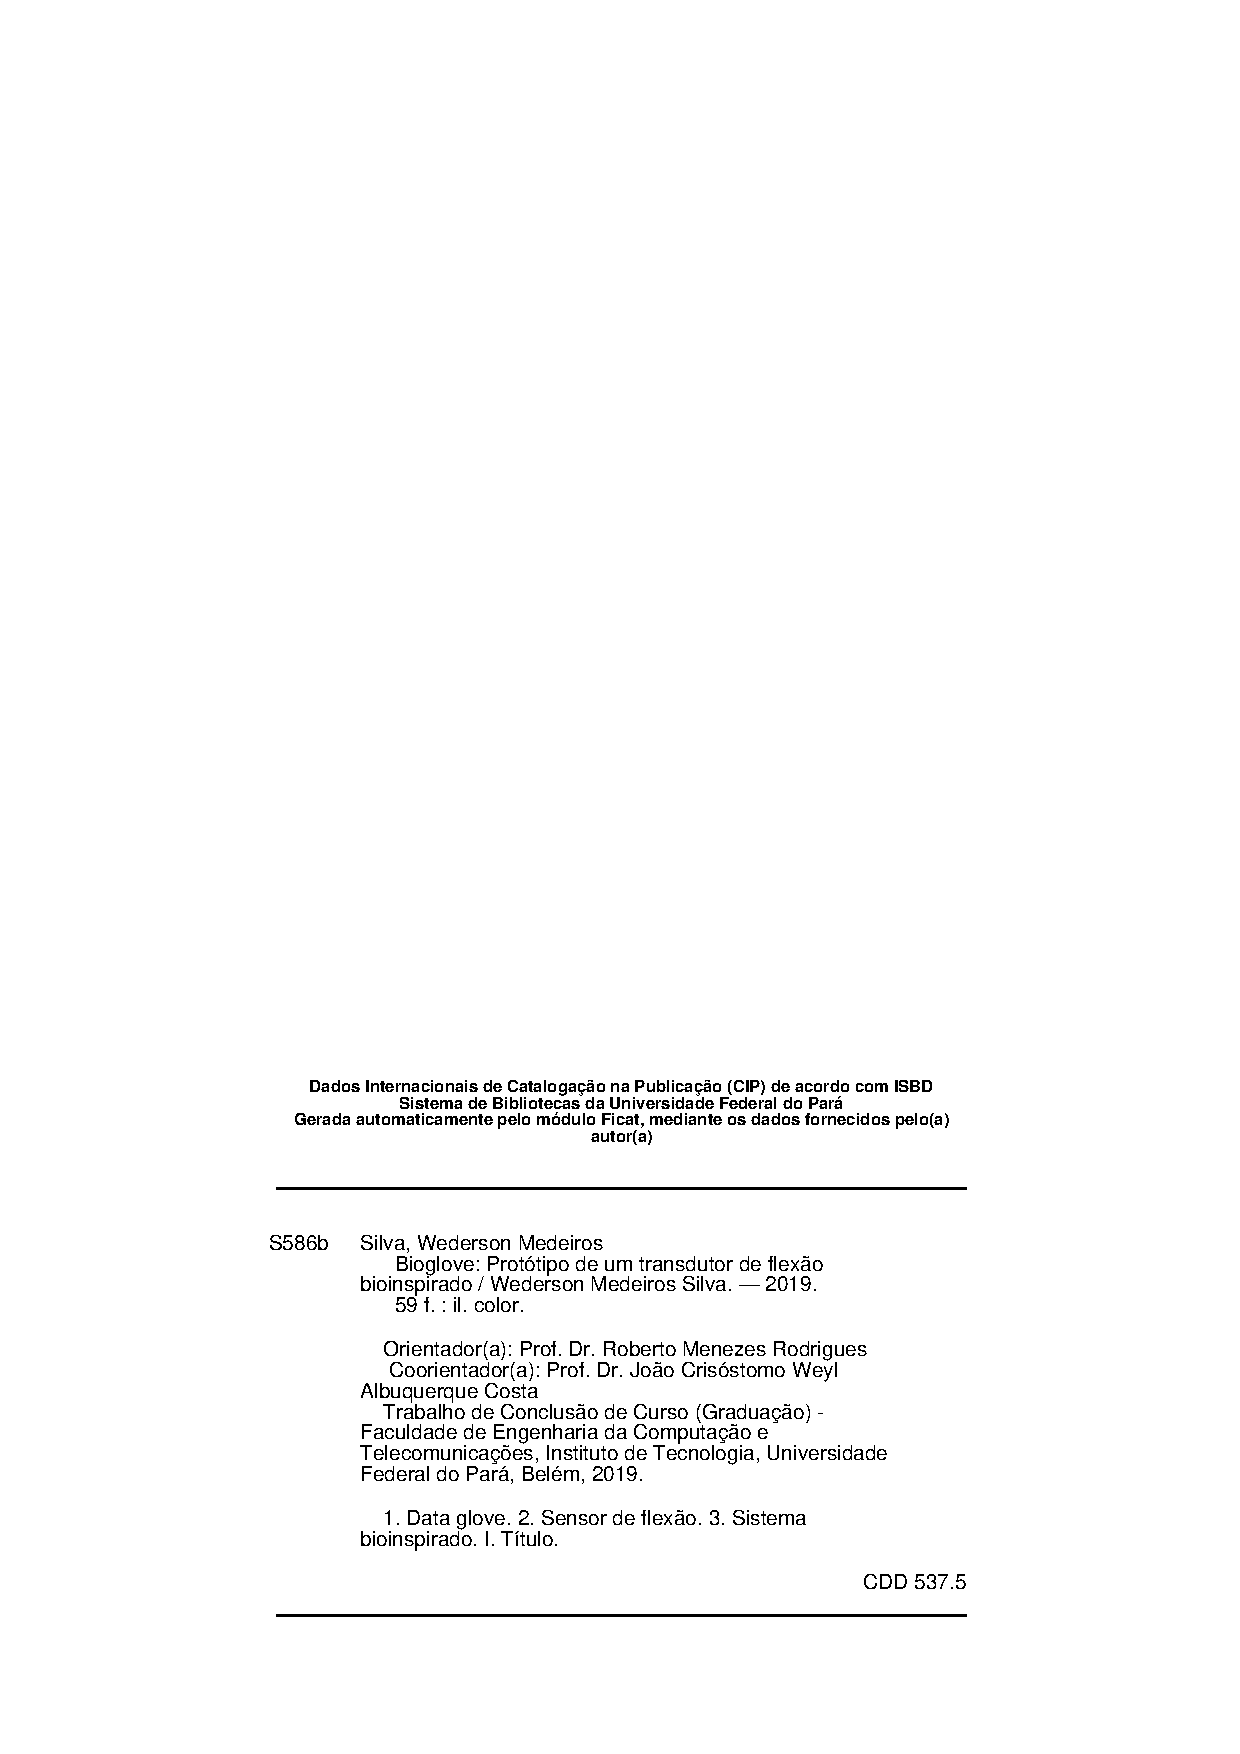
\includepdf{ficha_catalografica.pdf}
% \end{fichacatalografica}

%\begin{fichacatalografica}
%	\sffamily
%	\vspace*{\fill}					% Posição vertical
%	\begin{center}					% Minipage Centralizado
%	\fbox{\begin{minipage}[c][8cm]{13.5cm}		% Largura
%	\small
%	\imprimirautor
%	%Sobrenome, Nome do autor
%	
%	\hspace{0.5cm} \imprimirtitulo  / \imprimirautor. --
%	\imprimirlocal, \imprimirdata-
%	
%	\hspace{0.5cm} \pageref{LastPage} p. : il. (algumas color.) ; 30 cm.\\
%	
%	\hspace{0.5cm} \imprimirorientadorRotulo~\imprimirorientador\\
%	
%	\hspace{0.5cm} \imprimircoorientadorRotulo~\imprimircoorientador\\
%	
%	\hspace{0.5cm}
%	\parbox[t]{\textwidth}{\imprimirtipotrabalho~--~\imprimirinstituicao,
%	\imprimirdata.}\\
%	
%	\hspace{0.5cm}
%		1. Modo fantasma de segunda camada.
%		2. Taxa agregada.
%		3. \textit{Vectoring}.
%		4. EVM.
%		I. \imprimirorientador.
%		II. Universidade Federal do Pará.
%		III. Faculdade de Engenharia da Computação e Telecomunicações.
%		IV. \imprimirtitulo\\ 		
%	\end{minipage}}
%	\end{center}
%\end{fichacatalografica}
% ---
% ---

% ---
% Inserir folha de aprovação
% ---

% Isto é um exemplo de Folha de aprovação, elemento obrigatório da NBR
% 14724/2011 (seção 4.2.1.3). Você pode utilizar este modelo até a aprovação
% do trabalho. Após isso, substitua todo o conteúdo deste arquivo por uma
% imagem da página assinada pela banca com o comando abaixo:
%
% 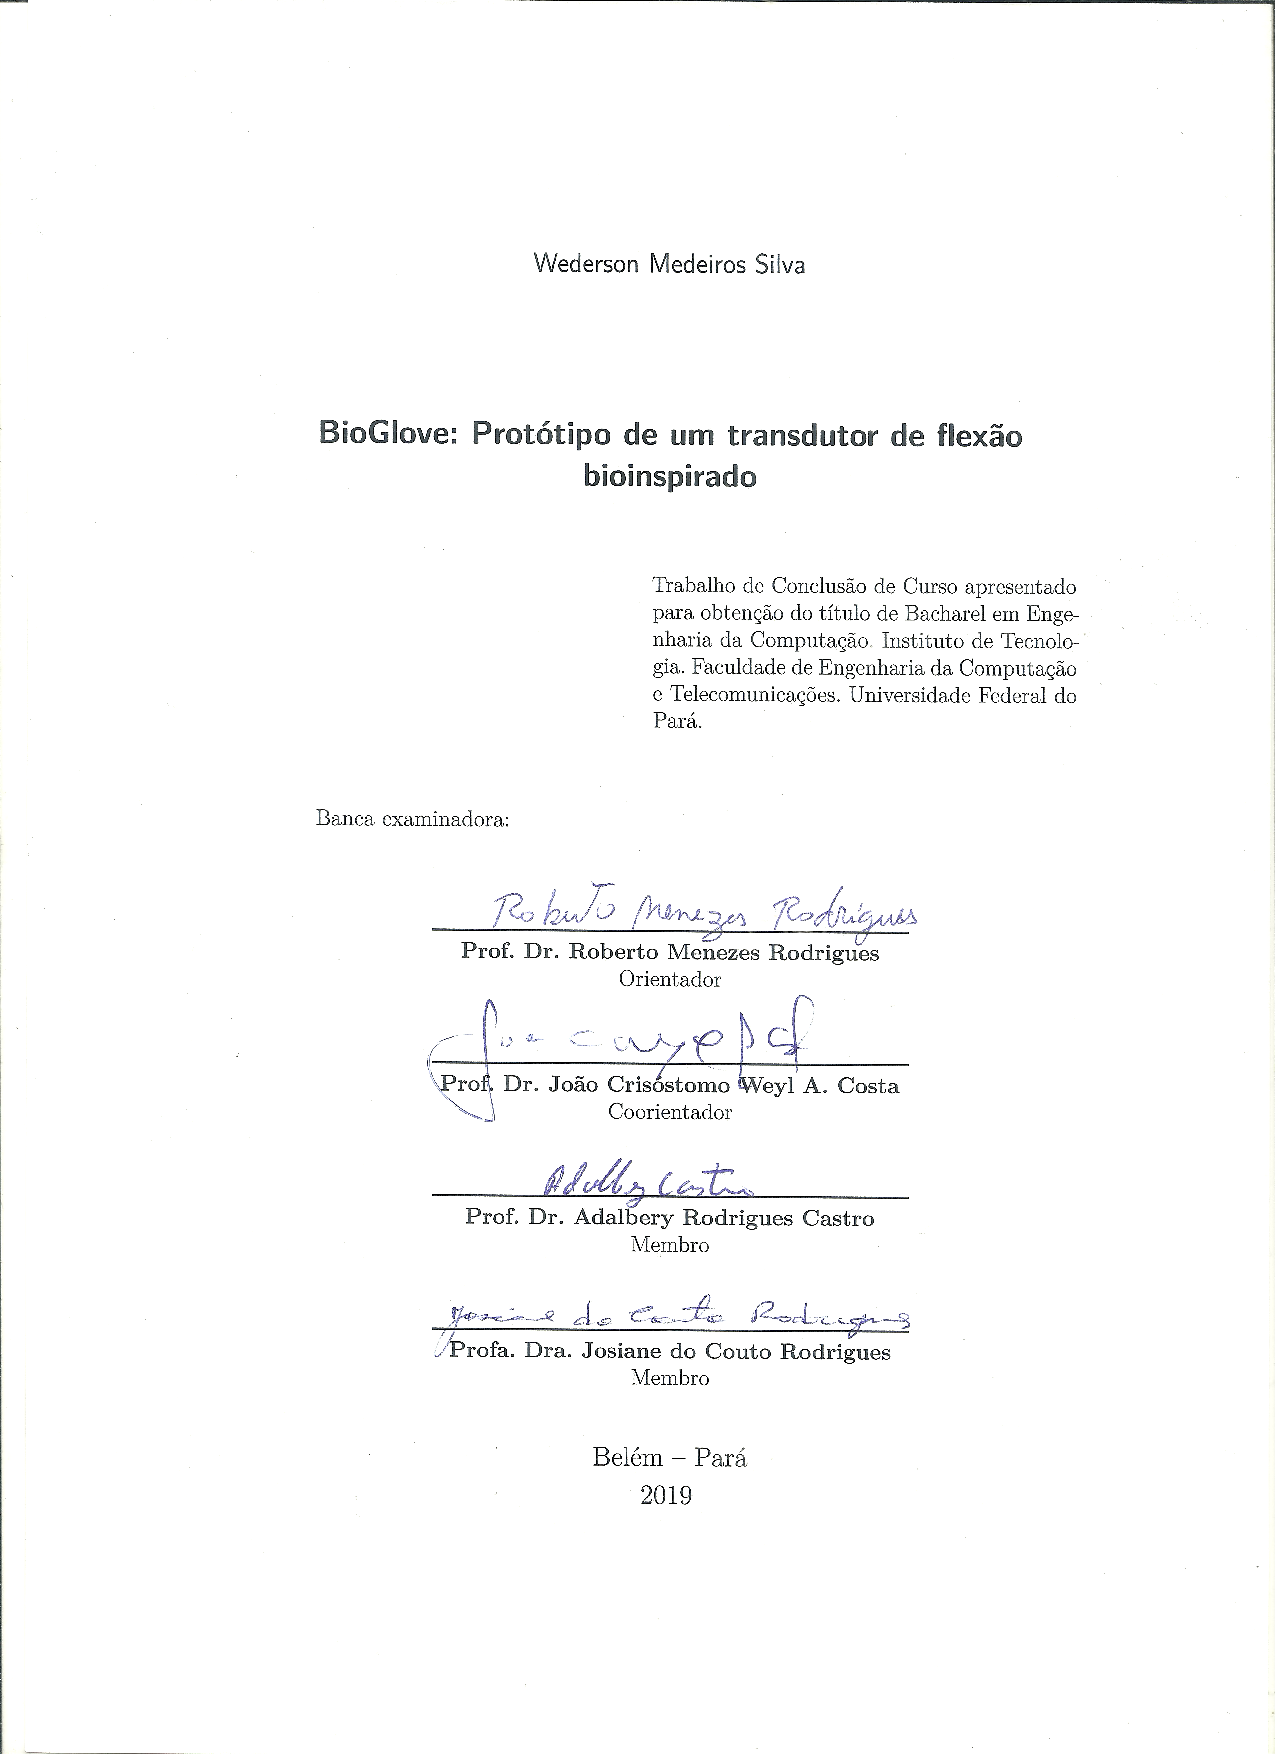
\includepdf{folhadeaprovacao.pdf}
%

%\begin{folhadeaprovacao}
%
%  \begin{center}
%    {\ABNTEXchapterfont\large\imprimirautor}
%
%    \vspace*{\fill}\vspace*{\fill}
%    \begin{center}
%      \ABNTEXchapterfont\bfseries\Large\imprimirtitulo
%    \end{center}
%    \vspace*{\fill}
%    
%    \hspace{.45\textwidth}
%    \begin{minipage}{.5\textwidth}
%        \imprimirpreambulo
%    \end{minipage}%
%    \vspace*{\fill}
%   \end{center}
        
%   Trabalho aprovado. \imprimirlocal, 11 de julho de 2019:

%   Banca examinadora: 
  
%   \assinatura{\textbf{\imprimirorientador} \\ Orientador} 
%	 \assinatura{\textbf{\imprimircoorientador} \\ Coorientador}
%	 \assinatura{\textbf{Prof. Dr. Adalbery Rodrigues Castro} \\ Membro}
%	 \assinatura{\textbf{Profa. Dra. Josiane do Couto Rodrigues} \\ Membro}
   %\assinatura{\textbf{Prof. Dr. Somebody else} \\ Convidado 2}
   %\assinatura{\textbf{Professor} \\ Convidado 3}
      
%   \begin{center}
%    \vspace*{0.5cm}
%    {\large\imprimirlocal}
%    \par
%    {\large\imprimirdata}
%    \vspace*{1cm}
%  \end{center}
  
%\end{folhadeaprovacao}
% ---

% ---
% Dedicatória
% ---
\begin{dedicatoria}
   \vspace*{\fill}
   \centering
   \noindent
   \textit{ Dedico este trabalho à minha mãe Eunice Pereira da Silva Conceição, mais conhecida como dona Zizi, que me criou superando dificuldades, com muito amor, fé, incentivo e com muita certeza em minha vitória. Além disso, também dedico este trabalho à minha Tia Elissandra Maria que foi a principal pessoa a acreditar e a dar todo tipo de suporte na construção do meu futuro acadêmico e profissional em Belém, mesmo nos momentos em que eu mesmo duvidei. } \vspace*{\fill}
\end{dedicatoria}
% ---

% ---
% Agradecimentos
% ---
\begin{agradecimentos}
Agradeço à Deus por abençoar constantemente meus passos nesse caminho que chamamos de vida, sempre me agraciando com saúde, oportunidades, conhecimento, pessoas excelentes, além de me permir evoluir a todo momento pessoal e profissionalmente.

Agradeço à minha família, minhas mães Eunice e Conceição, minhas tias Elissandra, Djanice, Ednice, Rosa e Hildete, meu Tio Denismar, meu Pai José Edson e minhas primas Ana Caroline e Jéssica, pelo apoio nas mais diversas formas e momentos, permitindo que eu esteja realizando o sonho da graduação. 

Agradeço ao meu orientador Prof. Dr. Roberto Menezes Rodrigues, ao meu coorientador Prof. Dr. João Crisóstomo Weyl A. Costa, além do Prof. Dr. Marco José de Sousa, pela paciência, orientação, credibilidade e conhecimento repassados a mim nos últimos anos.

Aos meus amigos Paulo Alexandre, Luan Assis, Celson Nakamura, Itamar Aguiar, Ítalo Cássio, Emanuel Araújo, André Lucas, Marx Miguel, José Vitor, Moisés Felipe e Waldeir Brito. Ademais minhas amigas Elizabeth Sousa, Aline Ayako, Damares Resende e Kárytha Nascimento, que foram pessoas-chave em algum ou em diversos momentos da minha graduação, sempre confiando em mim, dando conselhos, dicas ou apoio de diversas formas e com isso me trazendo o suporte e a confiança necessárias para superar os desafios que surgiram.

	Também agradeço aos amigos e colegas do Laboratório de Eletromagnetismo Aplicado (LEA) e do Laboratório de Prototipagem, Robótica e Otimização (LabPRO) que me ajudaram de forma direta ou indiretamente enquanto realizei minhas pesquisas nestes locais.


\end{agradecimentos}
% ---
% ---

% ---
% Epígrafe
% ---
\begin{epigrafe}
    \vspace*{\fill}
	\begin{flushright}
		\textit{``Talvez não tenha conseguido fazer o melhor, mas lutei para que o melhor fosse feito. \\ Não sou o que deveria ser, mas Graças a Deus, não sou o que era antes''. \\ (Martin Luther King)}
	\end{flushright}
\end{epigrafe}
% ---

% ---
% RESUMOS
% ---

% resumo em português
\setlength{\absparsep}{18pt} % ajusta o espaçamento dos parágrafos do resumo
\begin{resumo}
%\setlength{\parindent}{1.5cm}
%\indent
%\hangindent=3.7cm
	\hspace{1.5cm}Luvas embarcadas com sensores, também conhecidas como \textit{data gloves}, permitem interações com realidade virtual, robótica, controle, internet das coisas, telemedicina, entre outras. Essencialmente, tal interação se dá através do mapeamento do posicionamento das mãos bem como do grau de flexão dos dedos para determinados movimentos e ações dentro do ambiente na qual a luva está submetida. O custo da luva em muitos projetos se torna proibitivo por conta da tecnologia escolhida para tal mapeamento. No caso específico da  mensuração do grau de flexão dos dedos --- existem soluções baseadas em fibra óptica, tinta condutiva, sensores resistivos de flexão e potênciometros. Com o propósito de diminuir o custo de projetos que necessitam de uma \textit{data glove}, foi desenvolvida a BioGlove: uma luva de propósito genérico com sensores de flexão embarcados de baixo custo e inspirados na biomecânica dos dedos. Para o controle e comunicação da luva, foi utilizado uma placa microcontroladora que possui larga documentação e disponibilidade, além disso, foi desenvolvido um protocolo de comunicação e controle simplificados. O protótipo desenvolvido foi utilizado para o controle sem fio de um carrinho eletrônico e seu desempenho foi comparado com soluções comerciais documentadas na literatura. Os resultados mostraram que a \textit{Bioglove} apresenta desempenho similar às suas concorrentes especialmente nos quesitos precisão do mapeamento da flexão e consumo de energia.
 
	\textbf{Palavras-chaves}: \textit{Data glove}. sensor de flexão. sistema bioinspirado.
\end{resumo}

% resumo em inglês
\begin{resumo}[Abstract]
 \begin{otherlanguage*}{english}
\hspace{1.5cm}Gloves embedded with sensors, also known as data gloves, allow interactions with virtual reality, robotics, control, internet of things, telemedicine, and so on. Essentially, such interaction occurs through the mapping of hands position as well as the flexion degree of the fingers for certain movements and actions within the environment in which the glove is submitted. The cost of the glove in many projects becomes prohibitive because of the technology chosen for such mapping. In the specific case of measuring the degree of flexion of the fingers --- there are solutions based on fiber optics, conductive ink, resistive bending sensors and potentiometers. In order to reduce the cost of projects that require a data glove, was developed the BioGlove: a generic glove with low-cost embedded flexion sensors inspired by finger biomechanics. For the control and communication of the glove, a microcontroller board that has wide documentation and availability was used and a simplified protocol of communication and control was developed. The prototype developed was used for wireless control of an electronic car and its performance was compared with commercial solutions documented in the literature. The results showed that the BioGlove performs similarly to its competitors, especially in the flexion mapping and energy consumption requirements.

   \vspace{\onelineskip}
 
   \noindent 
   \textbf{Keywords}: Data glove. flex sensor. bioinspired system.
 \end{otherlanguage*}
\end{resumo}


% ---
% inserir lista de ilustrações
% ---
\pdfbookmark[0]{\listfigurename}{lof}
\listoffigures*
\cleardoublepage
% ---

% ---
% inserir lista de tabelas
% ---
\pdfbookmark[0]{\listtablename}{lot}
\listoftables*
\cleardoublepage
% ---

% ---
% inserir lista de abreviaturas e siglas
% ---
%\imprimirlistadesiglas
\begin{siglas}

	\item[3D]Tridimencional
	\item[A/D]Analógico-Digital
	\item[AGE]\textit{Abrams/Gentile Entertainment}
	\item[AM]\textit{Amplitude Modulation}
	\item[ASK]\textit{Amplitude-Shift Keying}
	\item[$cm$]Centímetro
	\item[CPU]\textit{Central Processing Unit}
	\item[E/S]Entrada e Saída
	\item[$GHz$]Gigahertz
	\item[$I$]Corrente elétrica
	\item[IDE]\textit{Integrated Development Interface}
	\item[$km/h$]Quilômetro por hora
	\item[$k\Omega$]\textit{Quiloohm}
	\item[LCD]\textit{Liquid Crystal Display}
	\item[LIBRAS]Linguagem Brasileira de Sinais
	\item[LiPo]\textit{Lithium-ion Polymer}
	\item[$m/s$]Metros por segundo
	\item[$mAh$]Miliampere hora
	\item[$MHz$]Megahertz
	\item[$mm$]Milímetro
	\item[NASA]\textit{National Aeronautics and Space Administration}
	\item[PCI]Placa de Circuito Impresso
	\item[PVC]\textit{Polyvinyl Chloride}			
	\item[$R$]Resistência elétrica
	\item[RAM]\textit{Ramdon Access Memory}
	\item[RF]Rádio frequência
	\item[ROM]\textit{Read Only Memory}
	\item[UDP]\textit{User Datagram Protocol}
	\item[USB]\textit{Universal Serial Bus}
	\item[$V$]Tensão
	\item[Wi-Fi]\textit{Wireless Fidelity}
	\item[$\Omega$]\textit{Ohm}

		% --- Parte baseado em: http://www.inmetro.gov.br/consumidor/pdf/Resumo_SI.pdf
	
\end{siglas}
% ---

% ---
% inserir lista de símbolos
% ---


%\begin{simbolos}
%  \item[$\alpha$] Contante de atenuação
%  \item[$\beta$] Contante de fase
%  \item[$\gamma$] Contante de propagação
%  \item[$\Gamma_{L}$] Coeficiente de reflexão na carga
%  \item[$\delta$] Constante da restrição de potência transmissão
%  \item[$\Delta_f$ ] Subcanais ou tons em Hz
%  \item[$ \Gamma $]  Gap de $RSIR$
%  \item[$ \Lambda $] Matriz que contém os elementos da diagonal principal de $\mathbf{H}$
%  \item[$\rho$] Máscara espectral utilizada pelo sistema DSL
  %  \item[
%  \item[${\sigma}^{2}$]  Densidade espectral de potência potência do ruído Gaussiano branco aditivo
%\end{simbolos}


% ---

% ---
% inserir o sumario
% ---
\pdfbookmark[0]{\contentsname}{toc}
\tableofcontents*
\cleardoublepage
% ---



% ----------------------------------------------------------
% GUIA DAYNARA
% ----------------------------------------------------------
%{\color{green}
%1- Introdução 
%
%Seção 1: Contexto:
%
%	-Contexto da tecnologia, contendo um histórico das evoluções ADSL – VDSL – G. Fast 
%	
%	-Apontar limitações dos sistemas em relação a transmissão (taxa agregada)
%	
%	-Quais as soluções que estão sendo investigadas
%	
%	-Uma das soluções é buscar modos de transmissão alternativos
%	
%	-Modo fantasma, split-pair e wire-shield 
%	
%Seção 2: Trabalhos relacionados (até onde eles abordaram)
%
%Seção 3: *Motivação:
%Por que pesquisar esta área e esse tema de modos alternativos de transmissão, onde poderia ser aplicados (5G, XG.), etc.;
%
%Seção 4: *Justificativa:
%Quais são exatamente as contribuições, o que eu fiz a mais em relação ao que já existe.
%
%Seção 6:*Objetivos
%
%Seção 5:*Resumo da metodologia
%
%Seção :*organização do trabalho
%}
%{\color{red}


% ----------------------------------------------------------
% ELEMENTOS TEXTUAIS
% ----------------------------------------------------------
\textual

\chapter{Introdução} % ou \input{arquivoexterno}
		
		\section{Contextualização}

%		A biologia inspira diversos projetos de engenharia. Na área da robótica, por exemplo, existe um robô em formato de salamandra que é capaz de se movimentar bem entre a água e a terra, há um pequeno robô inspirado em moscas que, devido ao seu formato, possui excelente decolagem vertical na hora do vôo. Existe ainda um robô que consegue escalar paredes através de um material adesivo que foi inspirado pela lagartixa \cite{pfeifer2007biorobot}. 

		A biologia intriga e inspira a humanidade desde a antiguidade. A diversidade dos seres vivos observáveis em suas mais diversas formas e capacidades geram questionamentos e pesquisas até os dias de hoje. 

		Já na Grécia antiga os pássaros, com a sua capacidade natural de voar, serviram de base para um dos primeiros projetos bioinspirados de que se tem notícia. Acredita-se que por volta de 400 a.C., Archytas (430 - 360 a.C.) que foi um matemático e astrônomo, inventou uma pomba mecânica que deveria voar \cite{livingstone2014greece}. Leonardo da Vinci (1452 - 1519 d.C.), provavelmente inspirado pelo projeto de Archytas, criou uma pomba mecânica que deslizava sobre um cabo ao mesmo tempo em que batia suas asas. Tempos depois, por volta do século XIX, um dispositivo muito parecido era vendido como brinquedo \cite{rosheim2006leonardo}.

		Dentre os materiais bioinspirados mais famosos está a tecnologia VELCRO${\textregistered}$ que foi baseada em uma planta chamada Bardana (\textit{Arctium lappa}). Essa planta possui uma série de pequenos ganchos que grudam em alguns tecidos. Por conta desse comportamento, o VELCRO${\textregistered}$ é composto de duas partes, os ganchos e as voltas \cite{velcro2019about}. 
		
		A área da robótica sempre teve um caráter bioinspirado. Existe um robô em formato de salamandra que é capaz de se movimentar bem entre a água e a terra. Há um pequeno robô inspirado na mosca que, devido ao seu formato, possui excelente decolagem vertical na hora do vôo. Existe ainda um robô que consegue escalar paredes através de um material adesivo que foi inspirado na lagartixa \cite{pfeifer2007biorobot}. 

		Não somente os animais e plantas vem servindo de base para projetos de engenharia. Partes especificas de sua estrutura corporal também tem sido foco de atenção. O próprio Leonardo da Vinci, a partir dos seus estudos em corpos humanos dissecados, chegou a construir modelos mecânicos de músculos, juntas, braços, que foram usados em muitas de suas invenções \cite{rosheim2006leonardo}. Com relação à mão, sabe-se que ela exerce uma importante função na interação do ser humano com diversas ferramentas do dia a dia --- desde o uso de instrumentos de trabalho como o martelo, serrote e a chave de fenda, até o ato de manipular a comida usando garfo e faca para se alimentar. Na área da tecnologia, muitos periféricos também necessitam da mão para serem controlados; é o caso do teclado do computador, do controle remoto da televisão e dos famosos \textit{tablets} e \textit{smartphones}.	Entretando, em aplicações de realidade virtual a imersão se torna ainda maior quando a interação é provida através de movimentos naturais do ser humano. Em um jogo de realidade virtual, por exemplo, será muito mais natural para o jogador alcançar um objeto virtual extendendo a sua mão, do que usar um \textit{joystick} para isso. Neste caso especificamente, o uso de uma luva com diversos sensores embarcados pode deixar a interação ainda mais real para o usuário. 
	

		\section{Estado da arte}

%		Como foi dito previamente, muitas pesquisas observam e se baseiam em sistemas da natureza para criar modelos a serem estudados. Inpirado pela forma humana, foi desenvolvido um robô bípede autônomo que procura imitar a marcha humana durante seu deslocamento, com o intuito de testar teorias de locomoção e eficiência de movimento. Tal robô, possui pernas e braços muito maiores do que o seu torso, se comparado ao corpo humano, mas seu movimento é semelhante ao nosso. Durante a caminhada do robô quando, por exemplo, a perna direita está à frente da perna esquerda, o braço esquerdo fica à frente do braço direito e vice-versa. Durante os testes, o robô conseguiu se locomover à uma velocidade de até 0,44$\,m/s$ (1.58$\,km/h$), com marcha relativamente estável. Dados mostraram que essa técnica mostrou uma eficiência de energia mecânica semelhante à de um ser humano, e com isso se estima que esse método ajudará a construir robôs caminhantes mais simples, eficientes, fáceis de controlar e mais práticos. Entretanto, seu custo ficou estimado em torno de 10 mil Dólares, a estrutura não se mostrou estável por longos períodos e a caminhada acontecia como esperado em 30\% do tempo \cite{collins2005walkrobot}.

%		Baseado em nossa biomecânica, existe um estudo de mapeamento dos movimentos do braço humano para controle de um braço robótico, onde os movimentos de flexão e extensão de um dos dedos e do pulso são adquiridos através de dois sensores resistivos de flexão comerciais, e um acelerômetro é responsável por mensurar movimentos do cotovelo. Esses dados são processados por um microcontrolador que por sua vez controla 4 servo motores montados em uma estrutura semelhante à de um braço robótico. Tal estrutura busca copiar os movimentos do braço do usuário através de 3 movimentos, ou graus de liberdade, independentes \cite{syed2012armcontroller}. Neste estudo é possível verificar que há uma conversão dos sinais analógicos em sinais digitais de uma forma proporcional, porém limitada. Além disso, o autor sugere que futuramente sejam adicionados protocolos para transmissão sem fio do sinal, o que pode dar uma maior liberdade de aplicações.
		
		Luvas com sensores embarcados podem captar diversos movimentos das mãos. Como sinais sobre a flexão dos dedos, giro do pulso, ou até mesmo a altura da mão em relação ao solo. Com isso é possível realizar pesquisas ou criar produtos que permitam um comportamento mais natural do usuário durante o uso ou durante a realização dos testes. Dentre os produtos que ficaram famosos usando movimentos das mãos para controle, estão as luvas \textit{Data Glove} e a \textit{Power Glove}, ambas criadas nos anos 80. A primeira, foi desenvolvida por volta de 1986 e era usada para controlar um supercomputador, mas também foi utilizada pela \textit{NASA (National Aeronautics and Space Administration)} para controlar robôs. Usava fibra óptica e fotoresistores para saber as posições de cada dedo, onde de acordo com o nível flexão do sensor, a quantidade de luz que chegava ao fotoresistor era variada, indicando portanto a posição atual. Logo depois, por volta de 1987, uma licença foi comprada para desenvolver uma outra versão dessa luva, só que esta nova luva seria para uso do público em geral. Então, finalmente em 1989, através de uma parceria entre as empresas Mattel, Nintendo e AGE (\textit{Abrams/Gentile Entertainment}), foi lançada a \textit{Power Glove} que serviria para controlar jogos de videogames. Entretanto, diferentemente do sistema anterior, a \textit{Power Glove} buscou reduzir custos trocando a tecnologia baseada fibra óptica por placas com tintas condutivas que variavam suas propriedades quando eram torcidas \cite{dana1989powerglove}. 
	
		Mais atualmente, na área médica foi desenvolvido o estudo de uma luva adaptável para medir a flexão dos dedos de indivíduos com limitações nos movimentos da mão e dos dedos \cite{simone2004lowcost}. O trabalho visa ser de baixo custo, não limitar os movimentos naturais dos usuários, ser leve e de fácil aplicação e remoção. Tais requisitos servem para monitorar, da melhor forma possível, as atividades de pessoas com limitações de movimento em suas atividades diárias. Essa pesquisa utiliza sensores de flexão resistivos comerciais colados em cada um dos cinco dedos da mão. Usando uma espécie de caixa de conexões, um computador é ligado à todos os sensores e realiza a conversão dos sinais analógicos em sinais digitais. Os testes mostraram que apesar de os sensores responderem aos movimentos, ainda é preciso realizar uma calibração antes do uso, além de que alguns materiais adesivos que grudavam os sensores aos dedos, acabaram soltando após algum período de uso. Por ser uma aplicação que visa ser utilizada durante testes relativamente longos (cerca de 24 horas), a necessidade de se ter um computador conectado constantemente aos sensores pode, de certa forma, atrapalhar nas atividades de cada usuário durante os testes.		
		
		Ainda com foco na mão, a pesquisa de \cite{daeholee2009vision}, criou um controle remoto baseado na abertura dos dedos. O sistema processa imagens de uma câmera em busca de comandos pré-configurados que respondem à abertura de dedos da mão. Ou seja, mostrou-se a possibilidade de usar os movimentos da mão como um meio para controle remoto. Além disso, existem trabalhos como o de \cite{anbarasi2013deafmute} que usa uma luva sensorizada junto a outros componentes com o objetivo de traduzir gestos definidos na linguagem americana de sinais em texto e áudio. Dessa forma, espera-se haver uma melhor comunicação de pessoas surdas ou mudas com outras pessoas que não são familiarizadas com a linguagem de sinais. A captura de flexões e extensões dos dedos são realizadas por sensores de flexão resistivos comerciais, enquanto que as direções dos movimentos durante os gestos da mão, são captados por um acelerômetro e existem ainda sensores de toque responsáveis por ``sentir'' o toque em determinadas áreas. Todos esses sensores estão conectados a um microcontrolador responsável por reconhecer padrões de movimentos, gerar palavras e as converter em aúdio através de um módulo e um alto falante. Já \cite{kumar2012hci} busca uma interação humano-computador através do uso de uma luva sensorizada, com a qual é possível realizar ações no computador, como desenhar ou manipular objetos tridimencionais, através de movimentos da mão pré-determinados.
		
		Em outros casos, luvas sensorizadas podem ser usadas para o controle de equipamentos, para receber e transmitir diversas informações relevantes a cada caso, ou podem ter funções genéricas. Um exemplo de luva multi-propósito é a 5DT \textit{Data Glove Ultra}, que é uma espécie de luva sensorizada comercial capaz de capturar diversos movimentos da mão, usando sensores de flexão baseados em fibra óptica entre outros. É um produto que possui opção para transmissão de dados sem fio através de \textit{Bluetooth}, além de poder ser integrado à \textit{softwares} de captação de movimento e animação em 3D conhecidos no mercado. Além disso, possui seu próprio \textit{software} de diagnóstico, gerenciamento, calibração e gravação de dados \cite{5DT-ultra}. Todas essas características, fazem deste produto uma excelente ferramenta para realizar estudos sobre os movimentos das mãos, ou para o desenvolvimento e controle de outros produtos. Entretanto, seu custo pode chegar na faixa dos 1000 Dólares \cite{5DT-glove2019ebay}. Além do mais, adaptações do \textit{hardware} ou \textit{software} que se fizerem necessárias, provavelmente não serão permitidas pelos desenvolvedores que detém os direitos deste produto.

		Os trabalhos apresentados até aqui utilizam sensores comerciais para mensurar os movimentos de flexão dos dedos, ou no caso da 5DT \textit{Data Glove}, seu próprio sensor baseado em fibra óptica e de tecnologia fechada. Entretanto, existem pesquisas que buscam criar o próprio sensor de flexão. No trabalho de \cite{flores2014glovecontroller} foram criados sensores improvisados usando fios, espumas condutoras, fita adesiva e pedaços de folhas de alumínio. O desempenho de tais sensores foi comparado com sensores de flexão resistivos comerciais. Usando sensores improvisados, os autores estimam uma economia de até 90$\,\%$ na construção de uma luva sensorizada. Entretanto, os sensores criados produzem muito ruído, fazendo com que fosse necessário enfatizar bem cada movimento de flexão ou relaxamento dos dedos durante os testes. Ainda assim foi possível criar um sistema binário de respostas que enviava duas saídas, sensor relaxado ou sensor flexionado. Portanto, para aplicações nas quais fosse exigida uma precisão maior, usar este sensor improvisado poderia gerar respostas instáveis para a aplicação em uso.


%movimentar desenhos tridimencionais em computador \cite{5DT-ultra}, mensurar atividades de pessoas com limitações dos movimentos nos dedos \cite{simone2004lowcost} e até mesmo transcrever gestos em palavras baseado na linguagem americana de sinais \cite{anbarasi2013deafmute}. Existem produtos comerciais \cite{5DT-ultra}, projetos de baixo custo \cite{simone2004lowcost}, usados em pesquisas médicas \cite{michela2013rehab}, entre outros. 


%		Para flexionar os dedos das mãos, possuímos tendões que passam por dentro de polias. Quando o músculo atrelado à esses tendões de movimenta, obtém-se a flexão ou extensão dos dedos \cite{drricardocirurgiao}.

		
%		As funções atribuídas à essas luvas são variadas.		
		
		
		\section{Motivação e objetivos}

		Apesar da gama de possibilidades com o uso de luvas sensorizadas, o custo de montagem dos produtos comerciais de plataforma fechada é elevado. Muitos projetos utilizam pelo menos um sensor de flexão resistivo comercial em cada dedo, sendo que a compra de cada unidade desse sensor pode custar, em lojas \textit{online} especializadas, em torno de 130 Reais \cite{multilogicaflexsensor}. Além disso, produtos comerciais costumam ter um \textit{hardware} imutável e de difícil manutenção, pois somente equipes especializadas possuem o conhecimento técnico ou a autorização legal para efetuar modificações.

		Este trabalho propõe criar um protótipo de uma luva com sensores de flexão bioinspirados embarcados, placa microcontroladora e transmissor de dados. O sistema deve possuir um conjunto de \textit{software} e \textit{hardware} de código aberto, que seja mais flexível em relação à outros produtos, permitindo que o usuário tenha liberdade de realizar modificações que se adaptem às suas necessidades. O sistema criado é de propósito genérico, mas para testar suas funcionalidades, foi desenvolvida uma aplicação para controle de um carrinho através dos gestos dos dedos.

		Esse trabalho também propõe avaliar a viabilidade de um sistema transdutor de flexão inspirado no movimento dos músculos e tendões da mão, onde esse sensor será composto de materiais de baixo custo e de fácil acesso e será o único modelo de sensor de flexão a compor a luva desenvolvida.	
	
		\section{Organização do trabalho}

		O restante deste trabalho está organizado da seguinte forma:

		No capítulo 2 apresenta-se a mecânica que inspirou a construção do sensor, o funcionamento da aquisição dos movimentos, detalhes sobre o potenciômetro que é a peça chave do sensor, e por fim, as características do microcontrolador e transmissor utilizados.
		
		No capítulo 3 detalha-se o funcionamento do sensor, a adaptação do sensor na luva, o algoritmo de programação do \textit{software} que trata o sinal recebido, os ajustes que foram necessários, além do protocolo de comunicação criado. Ao final é explicitado como todo o sistema foi construído e montado.

		No capítulo 4 apresenta-se a análise dos resultados obtidos com a BioGlove, tomando como referência outras luvas desenvolvidas.

		Por fim, no capítulo 5 são apresentas as conclusões do trabalho.
		

%Contextualização; Estado da arte (se tiver); Motivação; O que vai fazer; Metodologia; O que terá no resto do documento;




	% --------------------- 
	%	REFERENCIAL TEÓRICO	
	% --------------------- 
	
	\chapter{Referencial Teórico}

		\section{Introdução}



		Produtos ou pesquisas relacionadas com luvas sensorizadas, buscam mensurar com precisão e da melhor forma possível diversos movimentos das mãos para que estes sejam utilizados em suas aplicações. Para que isso seja possível, geralmente existe uma cadeia de funcionamento, mas que não necessariamente seja uma regra à todos os casos. Essa cadeia se inicia com os movimentos da mão, passando pela correta captura desses movimentos, processamento, transmissão, recepção e finalmente chegando até a aplicação desejada. A Figura \ref{Fig:flowchart1} demonstra essa cadeia genérica, comum a diversos sistemas baseados em luvas sensorizadas.

		\begin{figure}[h!]
			\centering
			\caption{Funcionamento genérico de sistemas baseados em luvas.}
  		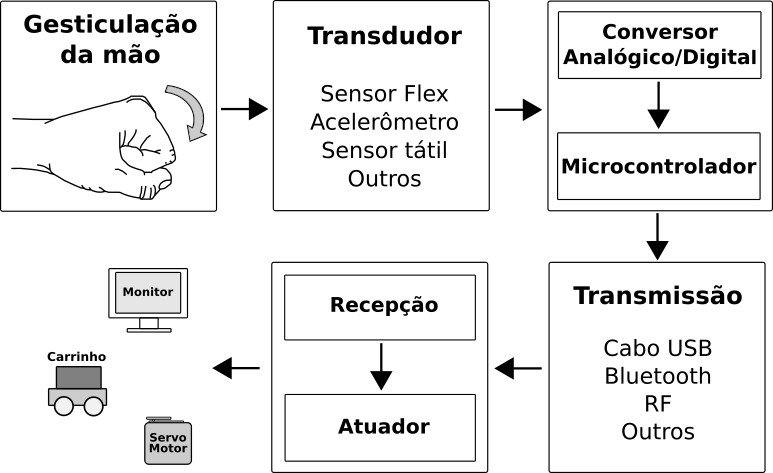
\includegraphics[width=9cm]{./figures/flowchart1.png}
  		\label{Fig:flowchart1}
			\fonte{Produzido pelo autor.}
		\end{figure}

		Durante os movimentos da mão, transdutores podem ser posicionados de uma forma que seja possível obter respostas sobre os graus de flexão de cada um dos dedos ou ainda de cada uma das juntas. Existe ainda a opção de colocar sensores no pulso ou no dorso da mão. Tais sensores podem ser usados para medir o giro pulso em relação ao braço ou a flexão da mão em relação ao pulso. Além do mais, outros sensores podem medir movimentos de aceleração entre uma posição e outra, ou até dizer a que altura a mão se encontra em relação ao solo.
		
		O uso exclusivo de sensores não é suficiente para as aplicações ou produtos, pois ainda é necessário que algum componente traduza e organize os dados enviados pelos transdutores. Dessa forma, será possível a correta leitura dos movimentos. Os microcontroladores são amplamente usados com esse objetivo, pois estes podem ser programados para interpretar os valores recebidos de cada sensor e para dar respostas compreensíveis dentro do contexto da aplicação. Ao receber os sinais analógicos de cada sensor, o microcontrolador ou algum componente conectado a ele, converte estes sinais para uma forma digital que poderá ser processada. 
	
		A decisão do que será feito com os sinais digitalizados que chegam até o microcontrolador dependerá de cada aplicação. Em alguns casos, mostrar estes valores em uma tela de computador será o suficiente, em outras opta-se por transmitir informações que indiquem os movimentos que estão sendo realizados pela mão do usuário. Nesse caso, as formas de transmissão podem ser as mais variadas seja através de fios ou não, e dentre as tecnologias de transmissão de informações sem fio estão \textit{Bluetooth}, Wi-Fi (\textit{Wireless Fidelity}) e outros tipos de rádio frequência.

		Após a transmissão do sinal, é necessário que algum componente receba e interprete tal sinal. Esse componente geralmente está ligado diretamente ao objetivo principal da aplicação. Por exemplo, no caso de uma aplicação que controle um atuador através dos movimentos da luva, provavelmente o atuador estaria conectado ao receptor do sinal. Em uma aplicação que vise mostrar os valores recebidos em uma tela de computador, o receptor poderia estar conectado à CPU (\textit{Central Processing Unit}) desse computador. Ou seja, o receptor da aplicação pode ser responsável não só pela interpretação do sinal recebido, como também pode controlar atuadores e enviar mensagens compreensíveis relacionadas aos sensores.

		Nas subseções a seguir serão apresentados mais detalhes acerca dos componentes relacionados a cadeia descrita acima. Começando por uma breve explicação sobre a biomecânica que possibilita a movimentação dos dedos, passando pelas formas de captura destes movimentos através de diferentes transdutores. Logo após haverá uma seção que descreverá o microcontrolador e suas funcionalidades, finalmente chegando à seção sobre formas de transmissão de sinal.



%		Entre os demais sistemas que buscam mensurar flexão e extensão dos dedos estão \cite{syed2012armcontroller} e \cite{michela2013rehab}. Estes e outros trabalhos, incluindo o trabalho proposto, nos quais utilizam luvas para auxiliar a captura dos movimentos dos dedos, costumam ter um bloco de funcionamento parecido ao da Figura \ref{Fig:flowchart1}.


		\section{Movimentação dos dedos} \label{sec:movimentacaodosdedos}


		Para que seja possível realizar diversos movimentos na mão, tendões funcionam como cordas que conectam os músculos do antebraço aos ossos da mão. Nos dedos, os tendões passam por dentro de uma série de polias, que formam uma espécie de túnel. Isso permite manter os tendões próximos aos ossos da mão, aumentando a força nos dedos e diminuindo o gasto de energia. Ao movimentar o dedo, o músculo se contrai para que o tendão deslize por entre as polias \cite{drricardocirurgiao}. De forma simplificada, para o dedo indicador, por exemplo, uma das pontas do tendão fica presa no osso (ou falange) localizado na ponta do dedo indicador e onde também há uma polia aproximando o tendão à essa falange. Ao longo das demais falanges também existem polias que aproximam o tendão e permitem seu deslizamento durante seus movimentos. Algo semelhante ao esquema demonstrado na Figura \ref{Fig:hand-tendon-flex1}, onde ao puxar o tendão no sentido indicado na figura, o dedo indicador fará o movimento de flexão também indicado.



		\begin{figure}[h!]
			\centering
  		\caption{Movimento do dedo através do tendão.}
  		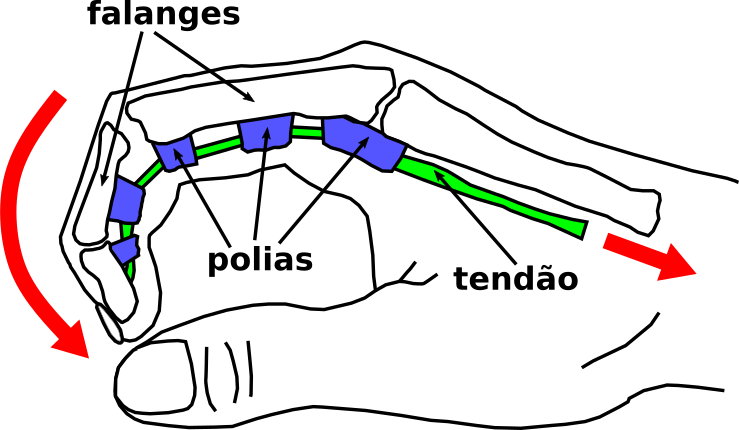
\includegraphics[scale=0.35]{./figures/hand-tendon-flex1.png}
			\fonte{Adaptado de \cite{drmarksurgery}.}
  		\label{Fig:hand-tendon-flex1}
		\end{figure}

		Essa biomecânica serve não apenas como fonte de informação, mas também é usada como inspiração para pequisas. Em \cite{hyunki2015exoglove}, por exemplo, mostra-se o funcionamento da \textit{Exo-Glove}, que é um tipo de luva responsável por auxiliar os movimentos dos dedos da mão de pessoas que sofreram alguma paralisia na região. O sistema guia tendões artificiais feitos com uma espécie de cabo de aço que partem e são controlados através de um módulo atuador posicionado na altura do braço, passando por um suporte próximo ao pulso, e ainda por correias de tecido para finalmente chegarem até os dedos. Usando todo esse aparato junto a um sistema de controle, os movimentos de flexão e extensão naturais dos dedos do usuário são auxiliados pelos cabos, que ficam em volta da luva formando uma espécie de exoesqueleto em volta de cada dedo. Dessa forma, é possível apoiar e dar movimentos mais firmes ao usuário. A Figura \ref{Fig:exo-glove-installed1} demonstra o sistema descrito.





		\begin{figure}[h!]
			\centering
			\caption{\textit{Exo-Glove} instalada em um cadeirante.}
  		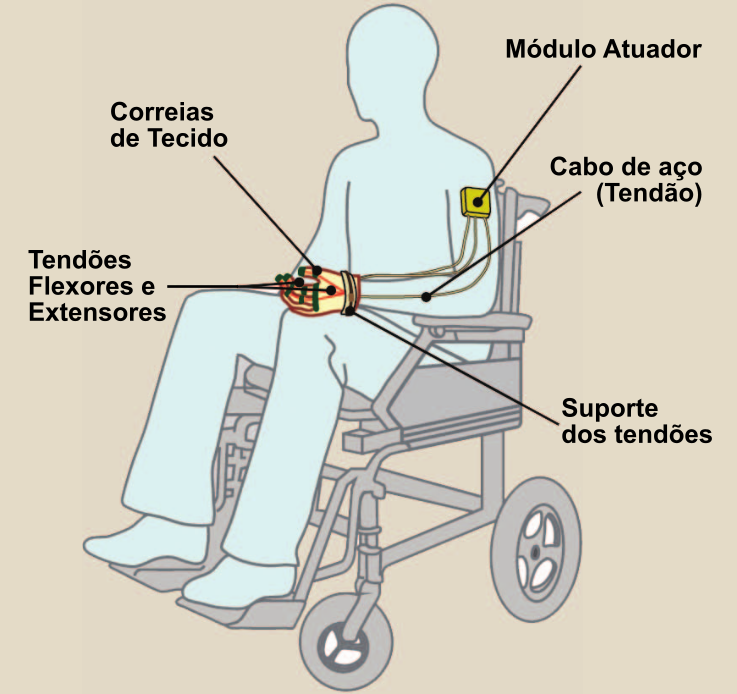
\includegraphics[scale=0.35]{./figures/exo-glove-installed1.png}
			\fonte{Adaptado de \cite{hyunki2015exoglove}.}
  		\label{Fig:exo-glove-installed1}
		\end{figure}
		
		\section{Captura de movimentos}



		Os circuitos eletrônicos trabalham com sinais elétricos, ou seja, com correntes e tensões elétricas. Sendo assim, para medir grandezas físicas que não envolvam eletricidade, é preciso o uso de transdutores, que são dispositivos que convertem uma forma de energia em outra. Os transdutores muitas vezes são usados para sensoriar determinadas grandezas, e por conta disso também são conhecidos como sensores \cite{ncb2012eletronicabasica}.

		Muitas pesquisas que buscam mensurar movimentos de flexão e expansão, usam sensores de flexão resistivos comerciais semelhantes a \cite{flexsensor}. Tal sensor possui uma resistência que é variada quando ele é torcido. Na mão, por exemplo, um sensor desses pode ser utilizado em cada ponto de flexão dos dedos, das juntas ou do pulso. Dessa forma, quando houver flexão em algum desses pontos, o sensor será torcido de acordo com o movimento, logo sua resistência também irá variar fazendo deste um sensor de flexão baseado na variação de resistência. O princípio funcional dos sensores de flexão pode também ser sintetizado através de componentes resistivos discretos como potenciômetros. 
		
		O potenciômetro é um componente eletrônico que permite, através do giro do seu eixo, a variação da resistência entre seus terminais. Eles são constituídos por um elemento de resistência, que pode ser de carbono ou fio de nicromo, sobre o qual corre uma lingueta, denominada cursor. Dentre as características do potenciômetro estão o valor máximo de sua resistência, seu número de voltas, seu grau máximo de giro (aproximado) e se ele é do tipo linear ou logarítmico \cite{ncb2012eletronicabasica}.

		A Figura \ref{Fig:potentiometer1} demonstra resumidamente o funcionamento do potenciômetro linear, onde a saída dos terminais é variada de acordo com o giro do cursor. Então, baseado nessa característica do componente e usando a lei de Ohm na qual $V = R.I$, dada uma corrente constante, ao variar a resistência teremos uma variação da tensão. Sendo assim, ao girar o eixo do potenciômetro, dependendo do sentido do giro, perceberemos um aumento ou diminuição da tensão naquele ponto, partindo de um ponto extremo com resistência mínima até o outro no qual a resistência deverá ser a máxima característica do componente. Dessa forma, é possível então fazer do potenciômetro uma espécie de sensor de giro.

		\begin{figure}[h!]
			\centering
  		\caption{Funcionamento do potenciômetro linear.}
  		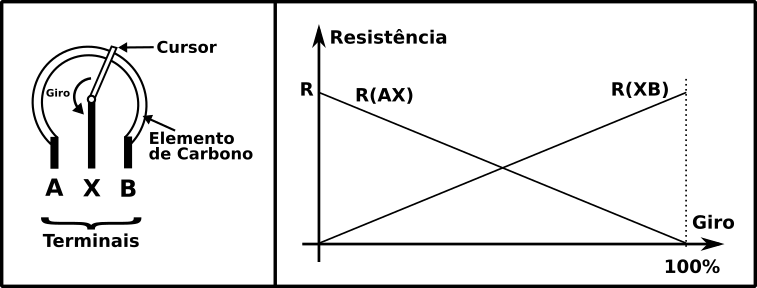
\includegraphics[width=12cm]{./figures/potentiometer1.png}
			\fonte{Modificado de~\cite{ncb2012eletronicabasica}.}
  		\label{Fig:potentiometer1}
		\end{figure}



%		Neste trabalho, propo\~e-se criar um sistema inspirado na biomecâmica dos dedos. Esse sistema deve mensurar movimentos de flexão e extensão dos dedos usando um transdutor mecânico com funcionamento semelhante ao sistema de tendões que ocorre nas mãos. 




%		\section{Potenciômetro}

		\section{Microcontroladores}

		Por volta da década de 80 surgiram os primeiros microcontroladores, dispositivos com microprocessadores, memória RAM (\textit{Ramdon Access Memory}), ROM (\textit{Read Only Memory}), clock interno, E/S (Entrada e Saída), entre outros. Por conta dessas características, os microcontroladores permitiram que projetos de dispositivos inteligentes se tornassem mais simples. Eles eram chamados por muitas vezes de computadores em um único chip \cite{pereiramicrocontroladores}. 

		Dentro do microcontrolador, ou conectado a ele, podem haver conversores analógico-digitais (A/D), que são utilizados justamente para converter sinais analógicos, como uma tensão, para sinais digitais nos quais o microcontrolador poderá ler e processar. Conversores A/D são muito úteis para aplicações de controle e monitoramento, pois muitos sensores (como sensores de temperatura, pressão, força, flexão, etc.) produzem sinais analógicos de tensão. Além disso, no microcontrolador existe uma comunicação serial de entrada e saída (E/S) que permite ao microntrolador se conectar à outro microcontrolador ou a um computador usando um cabo serial. Por conta dessa e outras características, se torna mais fácil desenvolver programas que visam a comunicação com outros componentes, enviando e recebendo dados de qualquer pino E/S do microcontrolador. \cite{ibrahim2011advanced}

		Existem ainda, soluções que buscam facilitar o uso do microcontrolador. O Arduino, por exemplo, é uma plataforma eletrônica de código aberto baseada em \textit{hardware} e \textit{software} fáceis de usar, possue ampla documentação e diversos projetos disponíveis gratuitamente pela internet. As placas Arduino são capazes de ler entradas como o acionamento de um sensor ou pressionamento de um botão, transformando essas entradas em diversos tipos de saídas como a ativação de um motor ou a publicação de algo \textit{online}. Essa placa pode ser programada usando sua IDE (\textit{Integrated Development Interface}), que por sua vez, envia as instruções necessárias para o microcontrolador instalado na placa \cite{arduinosite}. A placa vem com o microcontrolador modelo ATmega328 embarcado e está disponível em diversos tamanhos e modelos. Costuma ser utilizada para receber os sinais de transdutores, converter sinais analógicos em digitais, codificar sinais e enviá-los, entre outros. A Figura \ref{Fig:arduino-nano1} mostra a placa Arduino modelo Nano, que costuma ser usada em projetos de menor escala por conta do seu tamanho de aproximadamente 43$\,mm$ x 18$\,mm$.
	
		\begin{figure}[h!]
			\centering
			\caption{Placa Arduino modelo Nano.}
  		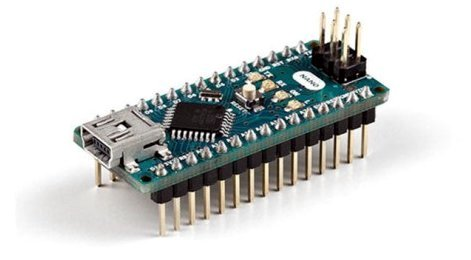
\includegraphics[width=12cm]{./figures/arduino-nano1.jpg}
  		\label{Fig:arduino-nano1}
			\fonte{Produzido pelo autor.}
		\end{figure}



%		Em \cite{michela2013rehab} o microcontrolador HC9S08QB8, da fabricante Freescale, consegue trabalhar na faixa de tensão requerida pelo projeto, consume pouca energia e juntamente ao transceptor MAX 1412 é capaz de diminuir a complexidade de transmissão, além de outras características. Já em \cite{anbarasi2013deafmute}, o microcontrolador ATmega 328 é utilizado para mostrar uma saída de texto em uma pequena tela LCD e juntamente ao chip TTS256 converter esse texto em som.
	


		\section{Comunicação sem fio}
		
		Após o processamento dos dados no microcontrolador, existem diversas formas de transmitir o sinal, e uma das formas mais simples é através de fios ou cabos ligados diretamente entre o transmissor e o receptor. Entretanto, a transmissão sem fio via rádio frequência pode ser uma das melhores opções, pois através dela é possível obter maior liberdade de movimentação entre o transmissor e o receptor dentro da área de alcance, sem a preocupação com problemas de mal contato ou emaranhar de fios, por exemplo. \textit{Bluetooth} e Wi-Fi são módulos que se comunicam a partir de frequências padrão, e trabalhar com eles pode facilitar a implementação de projetos, pois existe uma maior documentação, compatibilidade e disponibilidade desses módulos no mercado se comparado à outras formas de transmissão sem fio.
		
		Em projetos envolvendo luvas sensorizadas também é possivel observar essa variação nas formas de transmissão. No caso de \cite{solanki2013sign}, onde letras do alfabeto são interpretadas a partir de gestos de uma luva, a transmissão entre o microcontrolador e uma pequena tela de LCD (\textit{Liquid Crystal Display})  que mostra as letras é feita através de fios. O trabalho de \cite{syed2012armcontroller} busca controlar um braço robótico através de movimentos de uma luva, e nesta pesquisa os fios são conectados diretamente entre os pinos do microcontrolador e os servomotores que compõe o braço robótico.

		Dentre as soluções de transmissão sem fio a partir de uma luva sensorizada, uma das primeiras foi o sistema de ultrassom usado pela luva comercial \textit{Power Glove} que servia para controlar jogos de videogame por volta dos anos 80. Neste sistema, dois emissores de som ultrassônico instalados na luva enviavam as informações de controle para dois microfones localizados próximos à televisão \cite{dana1989powerglove}. Mais recentemente, em 2012, outra luva sensorizada comercial chamada DG5 VHand 2.0 foi aplicada na pesquisa de \cite{kumar2012hci} na qual a luva equipada com diversos sensores detectores de flexão e movimento, conseguia transmitir via \textit{Bluetooth} as informações necessárias para se comunicar e enviar comandos de controle para um computador.

		O uso de módulo RF (Rádio Frequência) 433$\,MHz$ pode ser outra opção para transmissão via rádio frequência. Estes módulos geralmente são compostos por um par contendo um transmissor (modelo XY-FST) e um receptor (modelo XY-MK-5V). O par opera com modulação AM (\textit{Amplitude Modulation}) e é considerado uma alternativa para projetos de baixo custo que queiram usar comunicação sem fio entre microcontroladores Arduino ou entre outros. O par de módulos pode alcançar até 200 metros sem obstáculos, usando antenas e dependendo da tensão aplicada \cite{institutodigitalrf}. A Figura \ref{Fig:tx-rx1} mostra um par desses módulos.


%		Em \cite{michela2013rehab}, a transmissão de sinal é realizada via rádio frequência, com o auxílio de um transceptor. Um transceptor é um sistema no qual estão presentes tanto o transmissor quanto o receptor de sinal em um mesmo módulo \cite{scott2017transceiver}.

		\begin{figure}[h!]
			\centering
			\caption{Módulos RF transmissor (esq.) e receptor (dir.).}
  		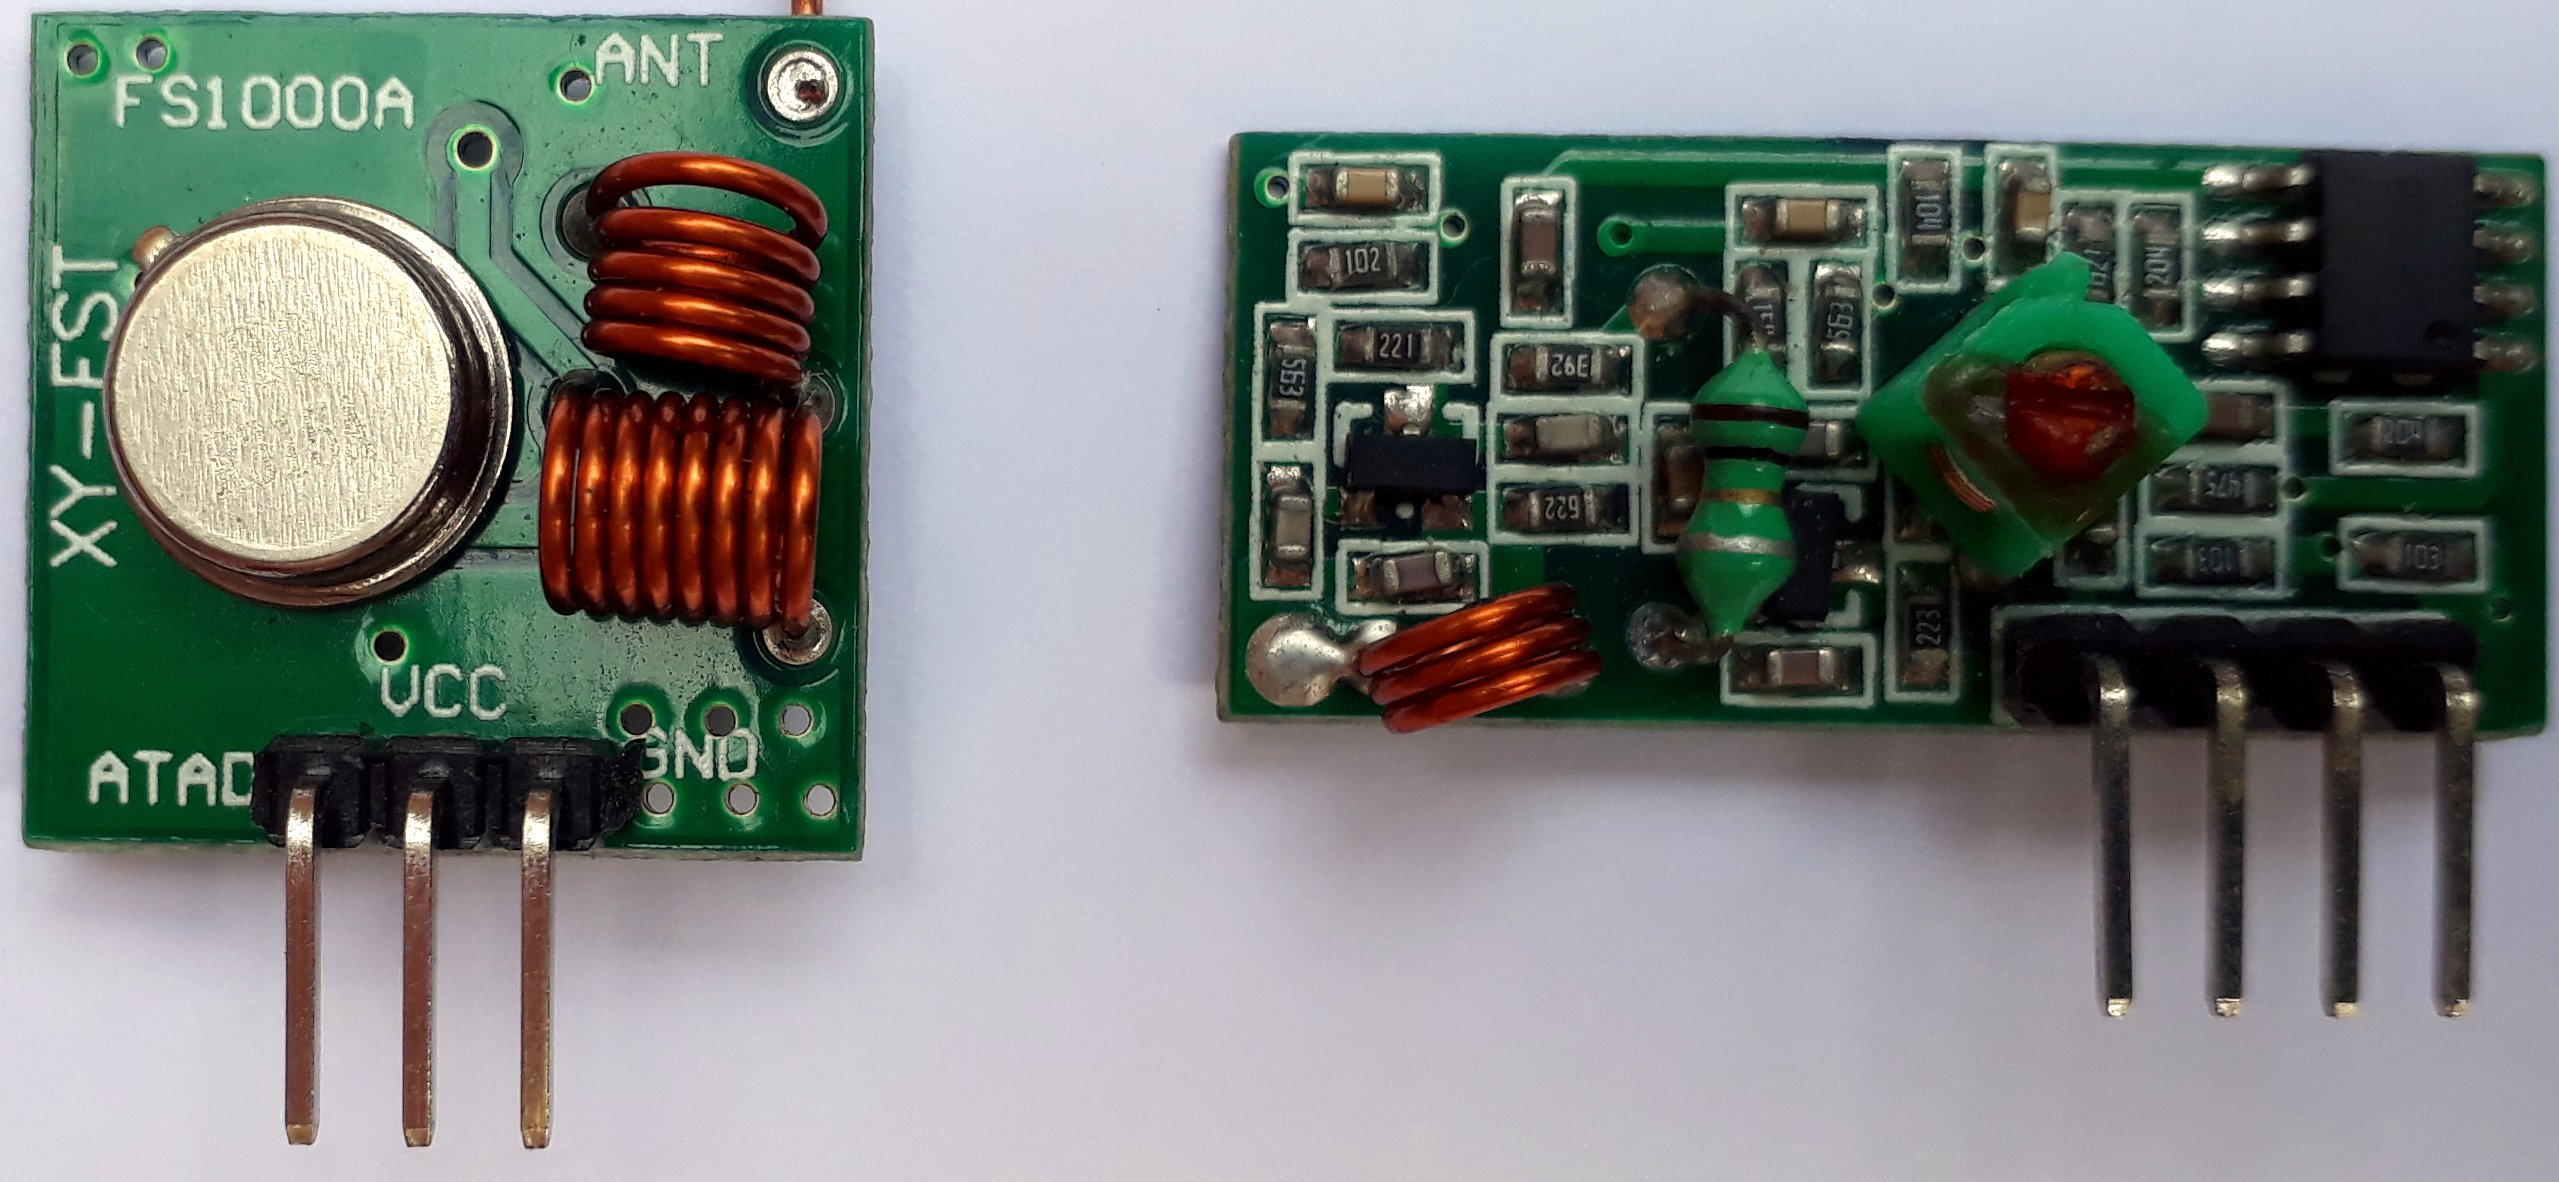
\includegraphics[width=12cm]{./figures/tx-rx1.jpg}
  		\label{Fig:tx-rx1}
			\fonte{Produzido pelo autor.}
		\end{figure}


%+++++++++++++++++++++++++++++++++++++++++++++++++++++++++++++
%
%			TRABALHO PROPRIAMENTE DITO	
%
%+++++++++++++++++++++++++++++++++++++++++++++++++++++++++++++
	
	\chapter{Desenvolvimento do Protótipo}

		\section{Introdução}
		
		O capítulo a seguir descreve a construção do protótipo, desde a biomecânica que inspirou o projeto até a montagem completa da luva. Serão apresentados detalhes sobre o funcionamento do sensor de flexão desenvolvido neste trabalho, processamento dos sinais no microcontrolador, desenvolvimento dos protocolos de comunicação e controle, chegando até a organização e montagem do sistema completo.
		
		Este capítulo está organizado em quatro seções. Na primeira delas explica-se a movimentação mecânica que permite ao transdutor captar movimentos de flexão e extensão dos dedos. A segunda aborda a programação do microcontrolador, mais especificamente o tratamento dos dados recebidos a partir dos potenciômetros, a calibração e o protocolo de comunicação desenvolvido. A terceira explicita como ocorre a transmissão do sinal, o protocolo de controle criado para o carrinho e o \textit{software} de recepção. A quarta e última seção explica-se detalhes sobre como o protótipo foi montado.



		\section{Transdutor de flexão}

			\subsection{Mecânica bioinspirada}

		Como foi explicitado previamente na seção \ref{sec:movimentacaodosdedos}, através dos tendões conectados entre as falanges e os músculos, é possível realizar movimentos de flexão nos dedos na mão. Baseado nessa biomecânica, foi desenvolvido um sistema mecânico que se comporta de forma semelhante e que objetiva criar um transdutor de flexão de dedos alternativo. 

		De uma forma resumida, no sistema natural de movimentação dos dedos, a extremidade do tendão está presa na ponta de uma das falanges do dedo, enquanto que sua extensão desliza por dentro de polias até o respectivo músculo do braço. No sistema alternativo desenvolvido, cada transdutor é composto por uma linha de náilon presa a um dos dedos de uma luva, essa linha é guiada através de pequenos segmentos plásticos até chegar no cursor de um potenciômetro. 
		
		Através da Figura \ref{Fig:bio-and-system} é possível observar semelhanças entre os dois sistemas. Na mão humana (Figura \ref{Fig:bio-and-system}(a)) o flexor superficial do dedo conecta as falanges até o músculo flexor superficial, e na luva (Figura \ref{Fig:bio-and-system}(b)) o fio de náilon representado em vermelho é o responsável pela conexão entre a ponta de um dos dedos e o potenciômetro. Na luva também é possível verificar que existem algumas polias, representadas por pequenos segmentos da cor azul, algo que não está representado na Figura \ref{Fig:bio-and-system}(a), mas que foi demonstrado previamente através da Figura \ref{Fig:hand-tendon-flex1}.

	\begin{figure}[!htb]
		 \centering
		 \caption{(a) Sistema biomecânico e (b) sistema desenvolvido.} 
		 \subfloat[]
		 {
			 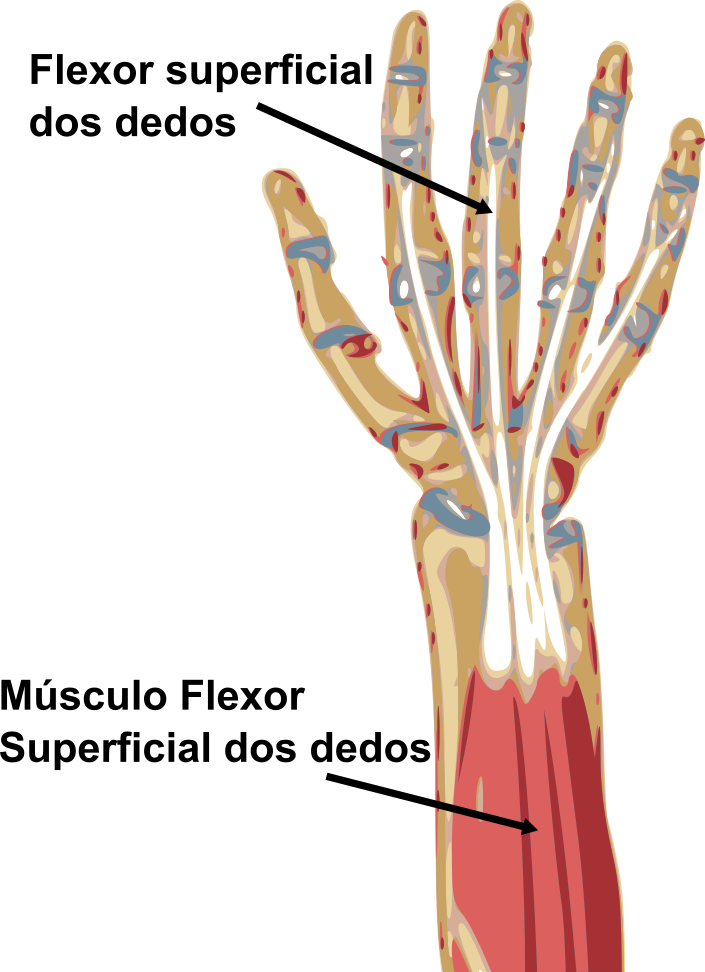
\includegraphics[width=5cm,keepaspectratio=true]{./figures/moore-biomechanic.png}
		 }
		 \centering
		 \subfloat[]
		 { 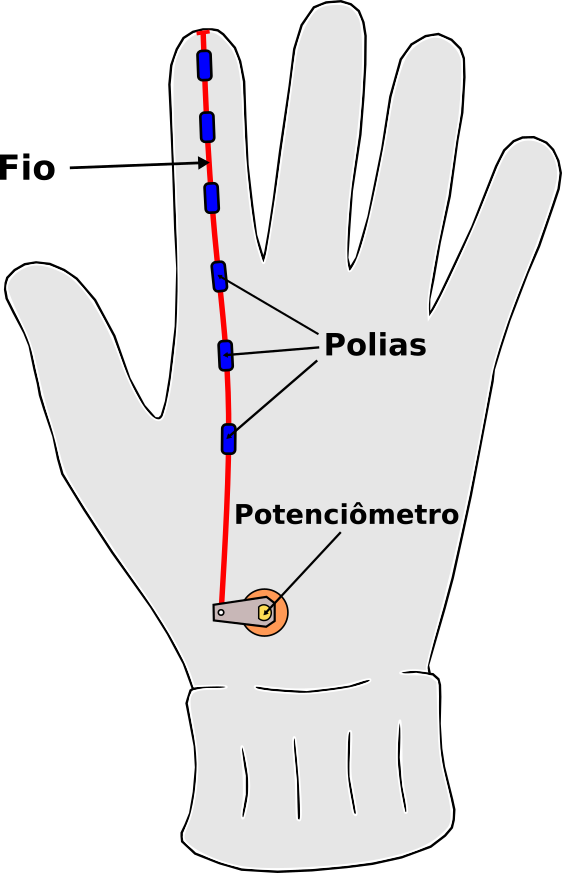
\includegraphics[width=4cm,keepaspectratio=true]{./figures/glove-wire-pot2.png}
		 }
		 \label{Fig:bio-and-system}
		 \fonte{(a) Adaptado de \cite{moore2013clinically} e (b) produzido pelo autor.}
	\end{figure}

		No sistema biomecânico, para que haja a flexão dos dedos, o músculo flexor se contrai, o tendão desliza por dentro das polias e isso faz com que o dedo realize o movimento de flexão \cite{drricardocirurgiao}. Ou seja, o músculo é o responsável por puxar o tendão quando o dedo se move. Após a realização de estudos sobre essa biomecânica, logo no início do trabalho foi formulada a hipótese de que durante a flexão de um dedo, poderia ocorrer um deslocamento proporcional de um fio sobre a mão. Um experimento foi desenvolvido para verificar tal hipótese. O primeiro passo do experimento foi prender uma das pontas de um fio na extremidade de um dos dedos da mão. O segundo foi deixar a mão inicialmente estendida (relaxada) com o dorso voltado para cima. Logo após, o fio foi posicionado no dorso da mão e o local de sua extremidade foi marcada. Essa configuração inicial do teste é demonstrado através Figura \ref{Fig:hand-wire-steady-and-flex}(a).

			Em um segundo momento, foi pedido que fosse realizado o movimento de flexão total dos dedos e verificou-se que o fio se movimentou em uma direção, criando um deslocamento \textit{d} do fio em relação ao ponto marcado anteriormente. Este segundo momento do experimento está demonstrado na Figura \ref{Fig:hand-wire-steady-and-flex}(b).
		

%\begin{figure}[H]
%	\caption{Cabo de pares trançados.}
%	\centering
%	\subfloat[Sem blindagem]{
%		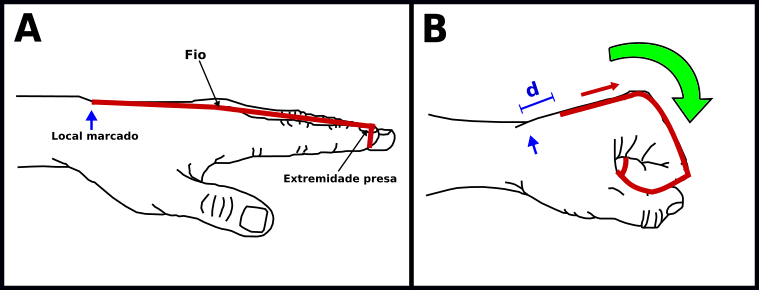
\includegraphics[width=7cm,keepaspectratio=true]{./figures/hand-wire-flex1.png}
%		\label{Fig:UTP}}
 
%	\centering
%	\subfloat[Com blindagem]{
%		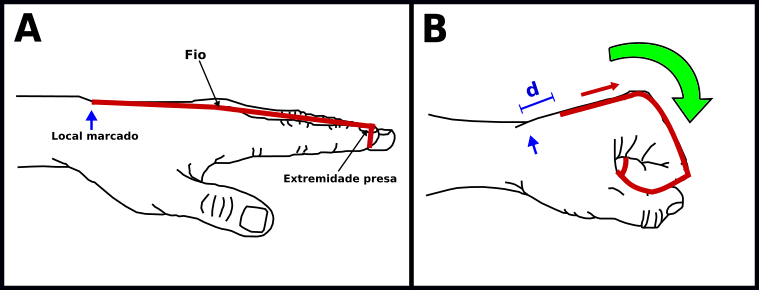
\includegraphics[width=7cm,keepaspectratio=true]{./figures/hand-wire-flex1.png}
%		\label{Fig:STP}}
%	\fonte{.}%
%	\label{Fig:Par}
%\end{figure}

\begin{figure}[!htb]
   \centering
   \caption{ (a) Mão em posição inicial e (b) Mão após flexão.}
   \subfloat[]
   {
     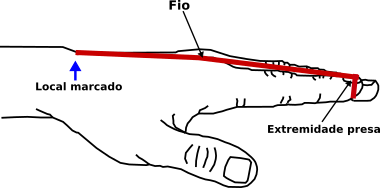
\includegraphics[width=8cm,keepaspectratio=true]{./figures/hand-wire-steady1.png}
   }
   \centering
   \subfloat[]
   { 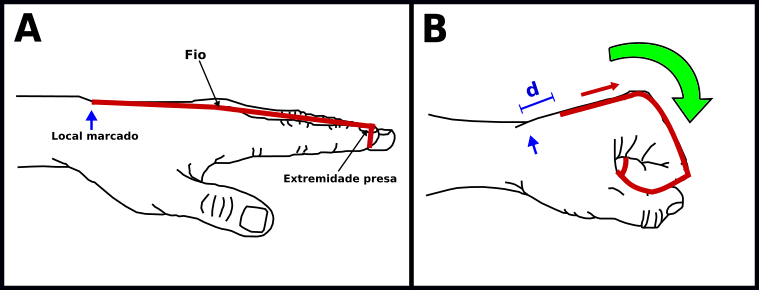
\includegraphics[width=6cm,keepaspectratio=true]{./figures/hand-wire-flex1.png}
   }
   \label{Fig:hand-wire-steady-and-flex}
   \fonte{Produzido pelo autor.}
 \end{figure}

		Examinando o resultado deste experimento, foi possível validar a hipótese formulada previamente. É válido também observar que quando compara-se esse sistema mecânico experimental com o sistema biomecânico natural, pode-se verificar que no sistema artificial o dedo do usuário é o principal responsável por exercer a força necessária para puxar o fio de náilon durante a flexão, enquanto que no sistema humano, o músculo do braço é o agente responsável por puxar o tendão e fazer com que o dedo flexione. Ou seja, em relação ao dedo, um dos sistemas é ativo e o outro é passivo.


		\subsection{Adaptação na luva} \label{sub:adaptacao-na-luva}


%		\begin{figure}[h!]
%			\centering
%			\caption{Captação do sinal.}
%  		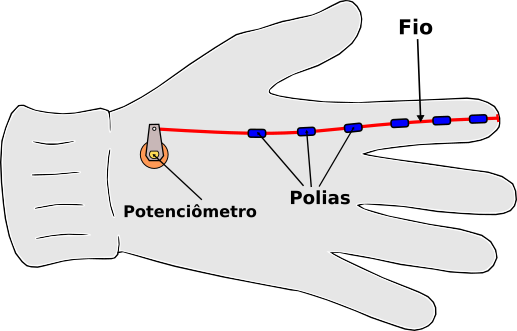
\includegraphics[scale=0.7]{./figures/glove-wire-pot1.png}
%  		\label{Fig:glove-and-transmitter1}
%			\fonte{Produzido pelo autor.}
%		\end{figure}


%		\subsection{Flexão e Extensão dos Dedos}

		Após examinar a movimentação mecânica descrita acima e com o objetivo de criar um sistema embarcado que fosse mais cômodo e estável para ser retirado e colocado na mão durante o uso, decidiu-se que todos os componentes do sistema seriam instalados em uma luva de algodão. Durante a instalação do sistema, um fio de náilon foi preso para cada uma das extremidades de cada dedo da luva. Além disso, cada um destes fios foi passando por dentro de polias plásticas costuradas previamente na luva. Na extremidade oposta, cada fio foi conectado à um cursor de um pequeno potenciômetro localizado no dorso da luva. Sendo assim, ao final dessa etapa de montagem, para os cinco dedos da luva, foram necessários cinco fios e cinco potenciômetros, além de diversas polias plásticas.

		Sabendo que durante o movimento dos dedos os fios se deslocam em uma distância proporcional à flexão do dedo, decidiu-se usar esse deslocamento para girar o cursor de um potenciômetro. Ou seja, toda vez que um dedo fosse flexionado, o cursor do seu respectivo potenciômetro seria girado proporcionalmente. Dessa forma, o potenciômetro juntamente com o fio funcionariam como um transdutor de flexão para cada dedo. Portanto, o funcionamento do transdutor é semelhante ao experimento demonstrado na Figura \ref{Fig:hand-wire-steady-and-flex}. 
		
		Entretanto, após a flexão do dedo, ao realizar o movimento inverso (extenção), não há força que movimente o fio de náilon e nem o cursor do potenciômetro de volta às suas posições iniciais e isso faz com que o transdutor funcione apenas uma vez. Então, visando solucionar este problema, um elástico foi instalado no cursor do potenciômetro para manter o fio tensionado e possibilitar que o sistema retorne à sua posição inicial. O sistema funciona da seguinte forma: Usando o elástico durante o movimento de flexão o cursor gira e estica o elástico, que estando esticado busca retomar sua posição de equilíbro realizando constantemente uma força contrária para girar o cursor de volta à sua posição inicial. Por conta do dedo ter mais força do que o elástico, o sistema se mantém dessa forma enquanto o dedo estiver flexionado. Este momento é demonstrado pela Figura \ref{Fig:glove-flex-and-extend2}(a) onde o elástico é representado pela cor azul e o fio de náilon pela cor vermelha.

		A partir do momento que o dedo realiza o movimento de extensão, o elástico puxa o cursor do potenciômetro e o fio de náilon simultaneamente. Com isso, o potenciômetro e o fio se movimentam em sentidos inversos ao que ocorreu durante o movimento de flexão. Tudo isso acontece enquanto o elástico estiver esticado o suficiente para exercer força sobre o cursor do potenciômetro. Dessa forma, o sistema consegue retornar ao seu estado inicial de equilíbrio, algo que é demonstrado na Figura \ref{Fig:glove-flex-and-extend2}(b).
		

	\begin{figure}[!htb]
		 \centering
		 \caption{ Movimentos da luva de (a) flexão e (b) extensão.} 
		 \subfloat[]
		 {
			 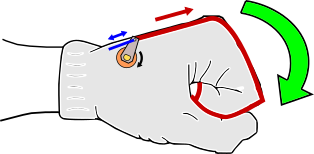
\includegraphics[width=6.5cm,keepaspectratio=true]{./figures/glove-wire-flex2.png}
		 }
		 \centering
		 \subfloat[]
		 { 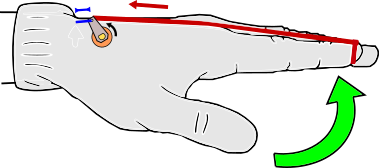
\includegraphics[width=7.5cm,keepaspectratio=true]{./figures/glove-wire-extend2.png}
		 }
		 \label{Fig:glove-flex-and-extend2}
		 \fonte{Produzido pelo autor.}
	\end{figure}


	
		\section{Programação do microcontrolador}

		Na luva, além do sistema transdutor de flexão bioinspirado, existe também um microcontrolador responsável por captar as variações de cada potenciômetro, digitalizar, processar e enviar para o módulo transmissor. Toda a programação é feita no computador através de uma IDE compatível com o microcontrolador escolhido e posteriormente o \textit{software} programado é carregado nele via USB (\textit{Universal Serial Bus}).  
		
		\subsection{Digitalização do sinal}

		Cada potenciômetro que compõe o transdutor de flexão desenvolvido só é capaz de fornecer um sinal de tensão analógico. Porém, um sinal analógico pode ter um número infinito de valores em um período de tempo \cite{forouzan2009comunicacao}. Por conta desse fato, uma das melhores formas para processar o sinal do potenciômetro é digitalizar cada sinal recebido. A placa Arduino, que foi a opção para este trabalho, é capaz de digitalizar sinais analógicos através de suas portas analógicas, e o microcontrolador embarcado fica responsável por converter cada variação de tensão do potenciômetro em valores inteiros entre 0 e 1023. 

		A partir daqui, para facilitar a abordagem do trabalho, cada dedo da luva e seu respectivo potenciômetro será representado por um número de 1 a 5, começando pelo dedo mínimo (1) até o polegar (5). Além disso, também serão definidas duas posições principais usadas para auxiliar a análise do movimento dos dedos. Posição A: Quando todos os dedos estiverem estendidos. Posição B: Quando todos os dedos estiverem flexionados. Estas duas posições estão representadas na Figura \ref{Fig:glove-flex-and-extend2} mostrada na subseção \ref{sub:adaptacao-na-luva}.

				
		\subsection{Calibração}

		Apesar de o microcontrolador ser capaz de digitalizar valores dos potenciômetros que variam de 0 a 1023, por conta da estrutura da luva, são utilizados apenas uma parcela desses valores, porque quando os dedos vem de uma posição extrema na qual todos os dedos estão extendidos (posição A) para a outra posição extrema na qual todos os dedos estão flexionados (posição B), ocorre apenas um giro parcial do cursor do potenciômetro e portanto apenas uma parte dos valores digitalizados é aproveitada. Além disso, mesmo quando os dedos estão em um mesmo grau de flexão, na grande maioria das vezes, os valores detectados para cada dedo são diferentes e existe uma certa instabilidade na leitura do potenciômetro mesmo que o dedos do usuário se mantenham estáveis. Por exemplo, para a posição A (estendida), por exemplo, o valor detectado no dedo mínimo (1) fica em torno de 191 (e não exatamente 191), enquanto que o anelar (2) apresenta, ao mesmo tempo, um valor em torno de 141. Isso ocorre por conta de alguns fatores: Existem pequenas diferenças nos valores de resistência mesmo entre potenciômetros do mesmo modelo (dentro da faixa de tolerância do fabricante); há diferença entre o tamanho dos dedos; as tensões aplicadas no fio de náilon não são iguais para todos os dedos; entre outras. Além do mais, devido à posição em que cada potenciômetro foi soldado na placa embarcada, alguns potenciômetros apresentam deslocamentos positivos enquanto outros apresentam deslocamentos negativos para um mesmo movimento.

		%	Durante o uso da luva, o potenciômetro não apresenta um valor fixo dada uma mesma posição. Ao invés disso, para cada posição detectável surge uma média de valores digitais relativamente estáveis. Então se, por exemplo, o dedo mínimo (1) está totalmente estendido (posição A), seu respectivo potenciômetro apresenta valores em torno de 191 (e não o valor exato de 191). Quando esse dedo é totalmente flexionado (posição B) seus valores ficam em torno de 616.

		
	%	\subsubsection{Deslocamento e resolução}

		Tendo em vista os problemas apresentados, o primeiro passo para calibrar o sistema foi conhecer quais seriam os valores apresentados para as posições A e B em cada um dos dedos, porque estes que são os graus máximos de extensão e flexão da BioGlove. Além disso, com o objetivo de se obter a resolução de cada dedo, foi necessário saber qual o número máximo de posições detectáveis durante o deslocamento entre as posições A e B.

		Para descobrir os valores de deslocamento, inicialmente cada potenciômetro teve seu valor digital médio anotado tanto para a posição A quanto para B, e posteriormente os valores de cada um dos dedos foram utilizados em (\ref{Eq:Desloca1}):

	\begin{equation}
			\Delta Pos 	= Pos B 	- 	Pos A ,
		\label{Eq:Desloca1}
	\end{equation}
sendo $\Delta Pos$ o valor de deslocamento de A para B. Com o módulo de $\Delta Pos$ é possível calcular o número de posições detectáveis (resolução) de cada dedo partindo da posição A até a posição B, através de (\ref{Eq:NPos1}):

	\begin{equation}
			NPos = |\Delta Pos| + 1.
		\label{Eq:NPos1}
	\end{equation}

		A Tabela \ref{Tab:deltapos} mostra os valores obtidos e calculados para cada um dos cinco dedos (potenciômetros) no deslocamento da posição A para a posição B.


	\begin{table}[H]
  	\centering
		\caption{Valores de A para B.}
    \begin{tabular}{c|cccc}
      \midrule
			Dedo	& PosA	& PosB	& $\Delta$Pos	& NPos	\\
      \midrule
			1 		& 191 	& 616 	& 		+425 		&	426		\\
			2 		& 140 	& 609 	& 		+469 		&	470		\\
			3 		& 774 	& 360 	& 		-414 		&	415		\\
			4 		& 728 	& 475 	& 		-253 		&	254		\\
			5 		& 670 	& 367 	& 		-303 		&	304		\\      
      \midrule
    \end{tabular}
    \label{Tab:deltapos}
    \fonte{Produzido pelo autor.}
	\end{table}
		
		Quanto maior for o valor de NPos na Tabela \ref{Tab:deltapos}, maior será a resolução e portanto mais preciso será o sensoriamento do dedo. Sendo assim, o anelar (2) é o dedo com maior potencial de sensoriamento, enquanto que o indicador (4) possui menor potencial. Observe ainda que os dedos 3, 4 e 5 apresentam deslocamentos ($\Delta$Pos) negativos, e isso acontece porque os valores de PosA são maiores do que PosB nesse grupo de potenciômetros. Entretanto, o tratamento dos deslocamentos negativos só se fará necessário durante a implementação do protocolo de comunicação a ser exposto a seguir.


			\subsection{Protocolo de comunicação}


		A resolução dos sensores bioinspirados apresentada até aqui é a máxima característica da BioGlove no momento, então qualquer aplicação pode se aproveitar desta capacidade para efetuar o sensoriamento de cada dedo e aplicar em sua pesquisa. Entretanto, visando exclusivamente a aplicação de controle do carrinho criada neste trabalho, esta resolução será diminuída porque o controle necessita apenas de algumas posições distintas em cada dedo. Além disso, objetivando diminuir o tamanho e a complexidade da mensagem de controle, decidiu-se reduzir ainda mais a faixa de valores possíveis que representam cada dedo (potenciômetro). 
		
		Como foi dito, para cada potenciômetro os valores máximos digitalizados são de 0 a 1023, sendo que a BioGlove aproveita apenas uma parte desses valores. Mas ainda assim, essa resolução continua desnecessariamente alta para a transmissão de sinal e controle do carrinho. Portanto, todos os valores possíveis de 0 a 1023 foram remapeados para valores inteiros entre 0 e 9 (10 níveis). Dessa forma, em uma mensagem numérica, seria preciso apenas 1 dígito para indicar o valor de flexão de um dedo. 
		
		A partir do remapeamento, seguindo o protocolo de comunicação, para criar uma mensagem são necessárias apenas duas informações: O número do potenciômetro; e o seu respectivo valor. Esse conjunto de valores é então concatenado em uma única mensagem ordenada de cinco dígitos, na qual a posição de cada dígito na mensagem representa cada um dos cinco dedos (vindo da esquerda para a direita) e o valor de cada dígito representa o valor do dedo naquele instante de tempo.  
		
		A Figura \ref{Fig:glove-create-msg1} exemplifica o protocolo de comunicação desenvolvido, onde uma mensagem é gerada a partir do posicionamente dos dedos na BioGlove. Neste exemplo, a mensagem ``69071'' indica que o dedo 1 (mínimo) possui valor o 6, o dedo 2 (anelar) possui valor 9 e assim sucessivamente até o dedo 5 (polegar) que possui o valor 1.


		\begin{figure}[h!]
			\centering
			\caption{Funcionamento do protocolo de comunicação.}
  		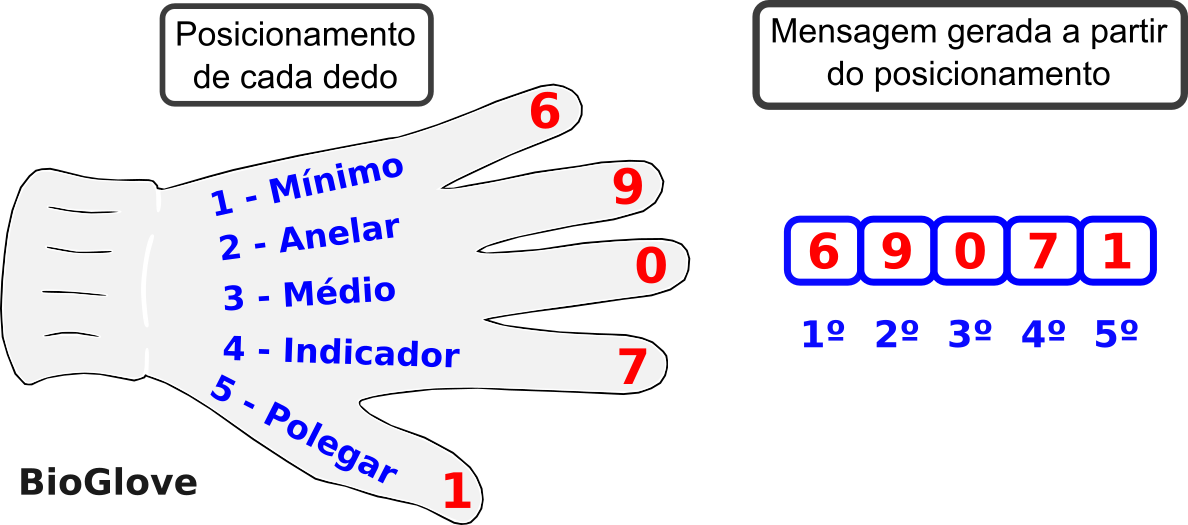
\includegraphics[width=12cm]{./figures/glove-create-msg1.png}
  		\label{Fig:glove-create-msg1}
			\fonte{Produzido pelo autor.}
		\end{figure}
		

		O protocolo de comunicação descrito repete o envio de mensagens constantemente com intervalos de tempo de microsegundos entre uma mensagem e outra, por mais que a mensagem atual seja a mesma enviada anteriormente.   
		
		Além de reduzir a resolução de cada potenciômetro para se adequar ao protocolo de comunicação, também foi necessário eliminar os deslocamentos negativos. Isso foi realizado com o intuito de criar um protocolo de controle mais simples e que funcionasse da mesma maneira para qualquer um dos dedos.

	 A chave para se adequar aos requisitos descritos até aqui foi a utilização da função ``map'' no código embarcado, isso porque esta função permite remapear uma faixa de valores em outra menor. Usando tal função, a faixa de entrada que inicialmente poderia variar entre 0 e 1023, foi remapeada para variar somente entre valores inteiros de 0 a 9. Além do mais, a função map também permite inverter sua saída de uma forma que os valores de entrada que variam de 1023 a 0 (decrescente) passam a variar de 0 a 9 (crescente). Com isso é possível eliminar os deslocamentos negativos.

	 Após remapear os valores digitais recebidos e eliminar os deslocamentos negativos, para fins de comparação, os novos valores também foram utilizados nas equações (\ref{Eq:Desloca1}) e (\ref{Eq:NPos1}), e os seus resultados foram adicionados à Tabela \ref{Tab:deltapos}, criando a Tabela \ref{Tab:deltaremap}:


	\begin{table}[H]
  	\centering
		\caption{Valores de A para B e remapeados (R).}
    \begin{tabular}{c|cc|cc|cc|cc}
      \midrule
			Dedo	&\multicolumn{2}{c}{PosA	(RA)} 	&\multicolumn{2}{c}{PosB (RB)}	&\multicolumn{2}{c}{$\Delta$Pos	($\Delta$R)}	&\multicolumn{2}{c}{NPos	(NR)}	\\
      \midrule
			1 		& 191 & (1)		& 616 & (5)		& 		+425 & (+4)		&			425	& (5)		\\
			2 		& 140 & (1)		& 609 & (5)		& 		+469 & (+4)		&			469 &	(5)		\\
			3 		& 774 & (3)		& 360 & (6)		& 		-414 & (+3)		&			414	& (4)		\\
			4 		& 728 & (3)		& 475 & (5)		& 		-253 & (+2)		&			253	& (3)		\\
			5 		& 670 & (4)		& 367 & (6)		& 		-303 & (+2)		&			303 &	(3)		\\      
      \midrule
    \end{tabular}
    \label{Tab:deltaremap}
    \fonte{Produzido pelo autor.}
	\end{table}
	
		Através da Tabela \ref{Tab:deltaremap} é possível observar a correspondência de valores antes e depois de remapeados. Por exemplo, o valor do potenciômetro apresentado no dedo 4 para PosA é de ``728'', entretanto o valor correspondente que será enviado na mensagem de controle é ``3''. Outro ponto a ser observado é a menor resolução dos valores remapeados (NR) quando comparado com a resolução anterior (NPos). Além disso, entre os valores de posição remapeados (RA e RB) não existem valores representados por mais de 1 dígito, o que era um dos requisitos para uma mensagem de transmissão mais simples. E por fim, nota-se que não existem deslocamentos negativos dentre os valores remapeados ($\Delta$R), outro objetivo da aplicação.

	
		\section{Transmissão, controle e recepção}

		\subsection{Introdução}

		Além de detectar diversos níveis de flexão dos dedos a partir do transdutor bioinspirado desenvolvido, a BioGlove também objetiva processar o sinal obtido e transmiti-lo sem fio para a aplicação alvo. Neste trabalho, a aplicação escolhida para ser controlada a partir da BioGlove é um pequeno carrinho elétrico, no qual ele deverá se movimentar de acordo com um conjunto de posições pré-determinadas dos dedos, ou seja, as direções de movimento do carrinho serão controlado através dos movimentos dos dedos.

		Para enviar o sinal até a aplicação, o sistema possui um módulo transmissor embarcado na BioGlove e um módulo receptor instalado no carrinho, que se comunicam sem fio através de sinais de rádio frequência. Entretanto, antes de enviar a mensagem é necessário que o microcontrolador organize as informações de uma forma que o módulo transmissor consiga ``falar''. Para isso uma biblioteca específica é usada durante a programação do microcontrolador embarcado na luva. Além disso, o microcontrolador embarcado no carrinho também precisa dessa biblioteca para ``entender'' o sinal que chega até o seu módulo receptor. Ou seja, a biblioteca permite que ambos os módulos se comuniquem entre si ``no mesmo idioma''. Uma vez que os módulos já consigam se comunicar adequadamente, ainda é necessário criar o conteúdo em si da mensagem que será enviada e o seu significado. Para isso neste trabalho foi desenvolvido um protocolo de comunicação específico para controlar o carrinho através dos gestos dos dedos. A Figura \ref{Fig:tx-rx-scheme1} demonstra esse processo de tradução, transmissão, recepção e recuperação da mensagem original através do uso dos módulos.

		\begin{figure}[h!]
			\centering
			\caption{Transmissão e recepção do sinal pelos módulos.}
  		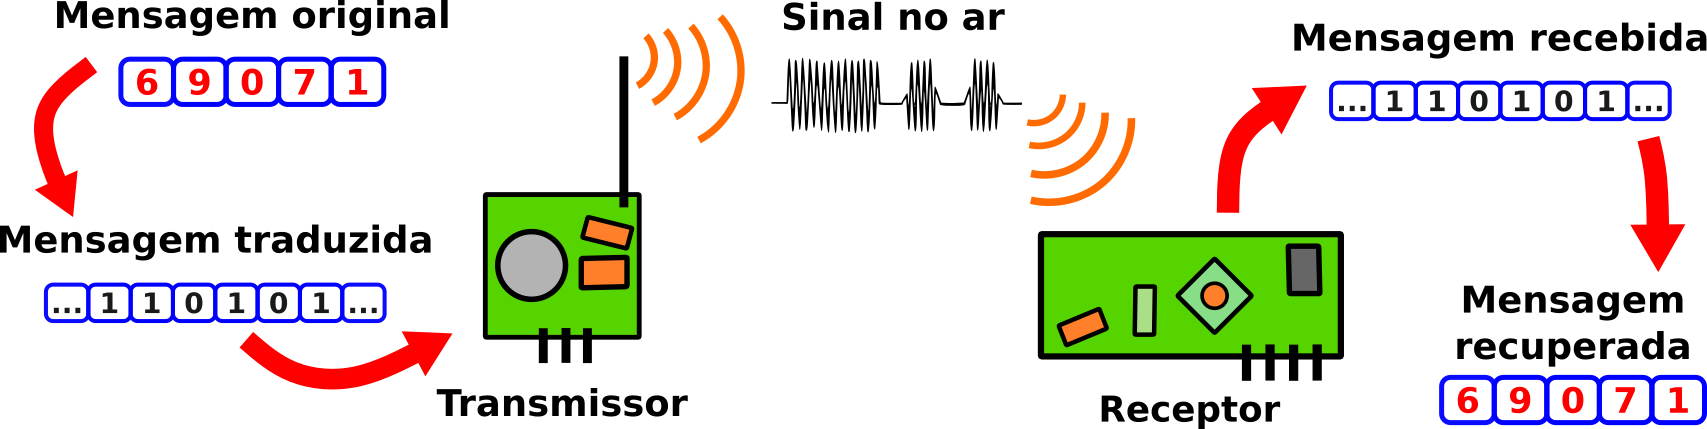
\includegraphics[width=14cm]{./figures/tx-rx-scheme1.png}
  		\label{Fig:tx-rx-scheme1}
			\fonte{Produzido pelo autor.}
		\end{figure}

		Nas subseções a seguir expoem-se mais detalhes sobre a programação dos microcontroladores embarcados na luva e no carrinho para que a transmissão do sinal e o controle sejam possíveis. A primeira seção é dedicada à biblioteca \textit{VirtualWire}, que está presente tanto no código de transmissão quanto no de recepção. Na segunda apresenta-se o código de transmissão que junta os valores dos potenciômetros e os envia ordenadamente. Na terceira seção explica-se como funciona o protocolo que foi criado para controlar o carrinho. A última seção destina-se ao \textit{software} de recepção e suas funções de controle de movimento que estão embarcadas no microcontrolador do carrinho.


		\subsection{\textit{VirtualWire}}


		\textit{VirtualWire} é uma biblioteca de comunicação para Arduino que possibilita a comunicação entre vários Arduinos usando transmissores e receptores de rádio frequência de baixo custo. Essa biblioteca permite o envio de mensagens curtas, sem endereçamento, retransmissão ou confirmação, como se fosse uma espécie de protocolo UDP (\textit{User Datagram Protocol}), usando modulação ASK (\textit{Amplitude Shift Keying}) \cite{virtualwiremanual}. 

		O uso dessa biblioteca nos códigos da IDE do Arduino permite abstrair tratamentos de envio e recebimento de dados necessários para a comunicação tais como, sincronização de padrões, balanceamento de bits 0 e 1, e checagem de erros \cite{virtualwirepjrc}. Dessa forma, para enviar e receber mensagens entre os módulos compatíveis, basta seguir os padrões de entrada e saída das funções descritas na documentação da biblioteca disponível gratuitamente na internet.

		Para o código embarcado no microcontrolador da BioGlove foi necessário definir, segundo os parâmetros da biblioteca, o pino de conexão do transmissor com o microcontrolador, a taxa de transmissão a ser utilizada, além do tamanho da mensagem que seria enviada. Porém, antes de efetivamente enviar a mensagem sempre é necessário converter a mensagem numérica em um dado do tipo \textit{string}, logo em seguida esta \textit{string} será transformada em um vetor de \textit{char}, que é o formato de dado aceito pela função de envio da \textit{VirtualWire}.

		No código embarcado no carrinho, a biblioteca é usada para receber as mensagens adequadamente, definindo-se alguns parâmetros como o tamanho da mensagem esperada, o pino de conexão do receptor com o microcontrolador e a taxa de transmissão, que deve ser a mesma definida previamente no \textit{software} embarcado na luva. Além disso, é necessário usar uma função que indica a chegada de uma mensagem, e quando isso acontece a mensagem recebida deve ser guardada em variáveis do tamanho correto, pois as mensagens são recebidas \textit{byte} a \textit{byte}. A partir desse ponto já é possivel usar a mensagem recebida da maneira definida pela aplicação.

		Uma vez que já existe um conhecimento básico acerca do funcionamento das funções e dos parâmetros da biblioteca necessários para cada aplicação, basta incluir a biblioteca em uma chamada logo no início do código de transmissão e do código de recepção.



		\subsection{\textit{Software} de transmissão}

		Inicialmente o \textit{software} embarcado no microcontrolador instalado na BioGlove tem como função a captura dos valores apresentados pelos potenciômetros e o remapeamento desses valores para uma faixa menor de valores. Esse período inicial do \textit{software} não será abordado nesta subseção, que é dedicada apenas aos trechos de código que caracterizam a forma de transmissão escolhida para esse trabalho.

		Como foi explicitado previamente, a estratégia de transmissão escolhida foi a de enviar uma mensagem de apenas 5 dígitos da luva para o carrinho, sendo que o valor de cada dígito representa o valor de cada potenciômetro (e consequentemente de cada dedo) naquele instante de tempo. Para que isso seja possível é necessário que o valores inteiros dos potenciômetros sejam concatenados lado a lado em uma ordem correta para formar uma única mensagem. Além disso, por conta de uma exigência da biblioteca \textit{VirtualWire}, ainda é necessário transformar esta mensagem numérica em um dado do tipo \textit{string} e posteriormente esta \textit{string} será dividida em um vetor de dados do tipo \textit{char}.	
		
		Uma das formas de converter valores inteiros em \textit{string} é concatenar o(s) valor(es) inteiro(s) com uma \textit{string} \cite{arduinostringadd}. Por isso, no código de transmissão, uma \textit{string} vazia é somada aos valores inteiros (que já foram remapeados) dos potenciômetros. Através deste método todos os valores serão concatenados e transformados em uma \textit{string} através de uma linha de código. Logo após, esta \textit{string} é transformada em um vetor de \textit{char} usando uma função chamada ``toCharArray''. A partir desse momento já é possível enviar a mensagem ao módulo transmissor usando a função ``vw\_send( )'' da \textit{VirtualWire}. O processo descrito até aqui está representado no pseudocódigo abaixo.		
%	// Inicia variaveis
%	string vazia = ""
%	string mensagem = ""
\lstset{language=C++,
%                basicstyle=\ttfamily,
                keywordstyle=\color{blue}\ttfamily,
                stringstyle=\color{green}\ttfamily,
                commentstyle=\color{red}\ttfamily,
								basicstyle=\footnotesize,
                morecomment=[l][\color{magenta}]{\#}
}
\begin{lstlisting}	
	// Recebe as posicoes de cada dedo
	int dedo1 = posicao_dedo1;
	int dedo2 = posicao_dedo2;
	int dedo3 = posicao_dedo3;
	int dedo4 = posicao_dedo4;
	int dedo5 = posicao_dedo5;

	// Concatena string + inteiros para obter uma unica string
	mensagem = string + dedo1 + dedo2 + dedo3 + dedo4 + dedo5;

	// Converte a string em um vetor de char
	mensagem = mensagem.toCharArray;

	// Envia o vetor de char
	vw_send(mensagem);
\end{lstlisting}

				
		\subsection{Protocolo de controle} \label{sub:protocolo-de-controle}

		O primeiro passo para a criação do protocolo de controle foi definir quais comandos seriam enviados para o carrinho. Somente para fins de demonstração, cinco comandos de movimento foram criados para o carrinho: ir para frente, ir para trás, girar para a esquerda, girar para a direita e parar.

		O segundo passo, foi definir quais gestos, ou combinações de gestos, realizados pelos dedos iriam servir para acionar algum desses movimentos do carrinho. Após a realização de alguns testes, foram definidos os seguintes gestos para controle: flexionar os dedos 2 e 3 simultanemanete, flexionar somente o dedo 4, flexionar somente o dedo 5, flexionar apenas o dedo 1 e não flexionar nenhum dedo.

		A relação entre os gestos e movimentos está representada na Figura \ref{Fig:glove-control-positions1}, que mostra a correspondência entre cada combinação de flexão dos dedos e seu respectivo comando para o carrinho. Apenas os dedos indicados em vermelho devem ser flexionados para validar o comando, e qualquer outra combinação realizada pelo usuário faz o carrinho parar.


		\begin{figure}[h!]
			\centering
			\caption{Comandos a partir de flexões e extensões para controle do carrinho.}
  		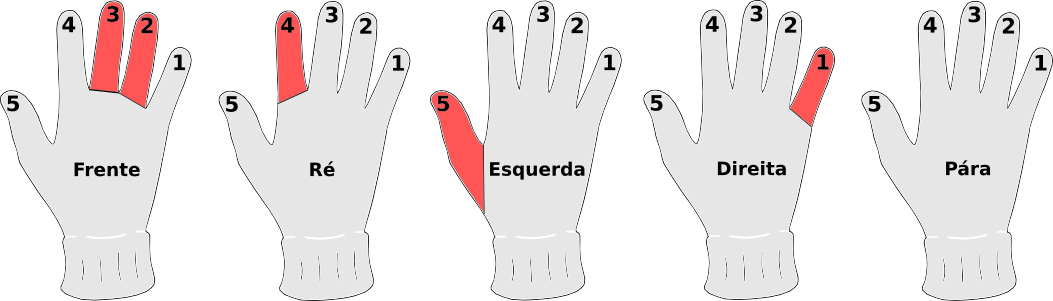
\includegraphics[width=14cm]{./figures/glove-control-positions1.png}
  		\label{Fig:glove-control-positions1}
			\fonte{Produzido pelo autor.}
		\end{figure}

		Detalhamentos sobre como o \textit{software} embarcado no carrinho consegue interpretar e reconher quais gestos foram efetuados pelo usuário da BioGlove serão explicitados na subseção a seguir que trata do \textit{software} de recepção.	

		
		\subsection{\textit{Software} de recepção}


		 O \textit{software} de recepção está embarcado em um microcontrolador instalado no carrinho elétrico. Este segundo \textit{software} é o responsável por capturar mensagens enviadas constantemente pela BioGlove, separar cada dígito da mensagem, interpretar cada valor e enviar o comando que vai fazer o carrinho se movimentar ou não. A forma como o código consegue realizar todas essas tarefas será discutida mais detalhadamente a seguir.
		
		A recepção dos sinais transmitidos a partir da BioGlove se dá através de um módulo receptor de rádio frequencia, conectado diretamente ao microcontrolador, que deve estar rodando a biblioteca \textit{VirtualWire} para interpretação adequada dos sinais recebidos.

		De forma resumida, o \textit{software} verifica se chegou alguma mensagem através da função ``vw\_wait\_rx( )'' nativa da \textit{VirtualWire}; em caso positivo, a mensagem em si é guardada em uma variável e o tamanho da mensagem é guadado em outra variável. Além disso, no momento em que a mensagem chega, uma condição controlada por um \textit{if} é acionada e se inicia um laço \textit{for} que recebe o tamanho da mensagem como parâmetro. Este laço é responsável por ler a mensagem \textit{byte} a \textit{byte} enquanto durar o tamanho da mensagem, e cada \textit{byte} lido é salvo em uma posição de um vetor. O pseudocódigo abaixo demonstra o fluxo descrito até aqui.
\begin{lstlisting}
// Aguarda receber alguma mensagem
chegou_mensagem = vw_wait_rx();

// Recebe a mensagem e o seu tamanho
byte msg = adquire_mensagem;
byte tamanho_msg = adquire_tamanho_msg;
	
// Verifica se ha mensagem, inicia o for para ler cada byte
if(chegou_mensagem){
	for (int i = 0; enquanto i < tamanho_msg; i++)
		byte_recebido[i] = msg[i];		
}
\end{lstlisting}

%		Um sistema receptor foi embarcado em um carrinho usando um segundo microcontrolador Arduino modelo Nano e um módulo receptor RF. Esse carrinho funciona com motores DC (\textit{Direct Current}) e todo o sistema é alimentado por uma bateria LiPo. 
		Usando o pseudocódigo apresentado e sabendo que a mensagem recebida contém 5 dígitos, percebe-se que a função \textit{for} irá rodar pelo menos 5 vezes, armazenando em cada interação o valor de um dígito em uma posição diferente do vetor \texttt{byte\_recebido[ ]}. Ou seja, após o fim do \textit{loop}, o vetor \texttt{byte\_recebido[ ]} terá os cinco dígitos da mensagem e seu respectivo valor. Seguindo essa lógica é possível concluir que o valor do dedo 1 estará contido em \texttt{byte\_recebido[0]}, do dedo 2 está em \texttt{byte\_recebido[1]}, continuando assim até o valor do dedo 5 que estará em \texttt{byte\_recebido[4]}.
		
		Após recuperar o conteúdo da mensagem, será necessário interpretar esse conteúdo de acordo com o protocolo de controle definido na subseção \ref{sub:protocolo-de-controle}. O primeiro passo foi criar e testar as 5 funções de movimentação do carrinho definidas previamente: \texttt{FRENTE( )}, \texttt{TRAS( )}, \texttt{ESQUERDA( )}, \texttt{DIREITA( )} e \texttt{PARA( )}. Ao chamar qualquer uma dessas funções, o carrinho passa a se movimentar na direção e sentido definidos. O segundo passo, para garantir a chamada da função correta baseada na mensagem recebida, foi criar cadeias de \textit{ifs} e \textit{elses} nas quais, quando satisfeitas as condições certas, a respectiva função é chamada fazendo com que o carrinho se movimente da maneira esperada. 
		
		A captura dos valores dos potenciômetros para alimentar corretamente as condições das cadeias de \textit{ifs} e \textit{elses} foi efetuada durante o desenvolvimento do \textit{software} através da anotação dos valores de todos os potenciômetros a cada grupo de gestos que compunha um comando da BioGlove. Com isso, criou-se a Tabela \ref{Tab:dedos-e-comandos1}, que mostra quais são os conjuntos de valores esperados para todos os dedos simultaneamente em cada comando, destacando os dedos flexionados (em vermelho). 
		
\begin{table}[H]
	\centering
  \caption{Conjunto de condições para validar comandos.}
  \begin{tabular}{r|ccccc}
		\midrule
\multicolumn{1}{c|}{Dedo} 					&       Frente			 & 				Trás				& 		Esquerda			 & 		Direita					& Para	\\
			 \midrule
			 Mínimo - 1    		& < 2   						 & < 2   							& < 2    						 &\textcolor{red}{> 1}&	-			\\
			 Anelar - 2    		&\textcolor{red}{> 1}& < 2   							& < 2  	 						 & < 2   							&	-			\\
			 Médio - 3    		&\textcolor{red}{> 3}& < 4   							& < 4   						 & < 4   							&	-			\\
			 Indicador - 4    & < 4   						 &\textcolor{red}{> 3}& < 4 							 & < 4   							&	-			\\
			 Polegar - 5    	& < 5   						 & < 5   							&\textcolor{red}{> 4}& < 5   							&	-			\\
		 \midrule
	\end{tabular}
  \label{Tab:dedos-e-comandos1}
  \fonte{Produzido pelo autor.}
  \end{table}

		A Tabela \ref{Tab:dedos-e-comandos1} é utilizada para saber qual a combinação de valores simultâneos em cada um dos dedos que satifaz as condições corretas e movimenta o carrinho na direção desejada. Sendo assim, para saber quais combinações de valores fariam o carrinho se movimentar para frente, é só observar a coluna ``Frente'' da tabela. Nesse caso, uma mensagem ``13422'' faria o carrinho seguir em frente porque a combinação de todos os dígitos respeita todos os valores da coluna ``Frente'' da tabela. Porém, uma mensagem ``11422'' não faria o carrinho ir para frente porque o segundo dígito desta mensagem não é maior que ($>$) 1.

		Outro ponto a ser observado na Tabela \ref{Tab:dedos-e-comandos1}, é o destaque em vermelhor dos dedos que são flexionados durante um determinado comando. Observe que a coluna ``Direita'', que corresponde a combinação necessária para movimentar o carrinho para a direita, destaca o dedo 1 (mínimo) que é justamente o único dedo que deve ser flexionado para fazer o carrinho ir para a direita. Ademais, em todas as colunas em que aparecem destaques em vermelho o simbolo de comparação é o maior que ($>$), isso foi feito para destacar nas linhas de código do \textit{software} quais são os dedos flexionados que são esperados para aquele comando, dessa forma é mais fácil criar ou alterar comandos baseados na flexão dos dedos.

		Um último ponto sobre a Tabela \ref{Tab:dedos-e-comandos1} é que se ela for comparada com a Figura \ref{Fig:glove-control-positions1}, será observado que são compatíveis entre si, porque tanto na Tabela \ref{Tab:dedos-e-comandos1} quando na Figura \ref{Fig:glove-control-positions1} os mesmos dedos flexionados estão destacados em vermelho representando os gestos necessários para efetuar cada comando. Além disso, qualquer outra combinação além das especificadas na tabela, fará o carrinho ficar parado e os erros que ocorrem durante a transmissão de dados são tratados pela biblioteca \textit{VirtualWire}. Isto conclui o protocolo de controle do carrinho.



		\section{Montagem do protótipo}

		
				\subsection{Introdução}	
				

		O \textit{design} do protótipo foi baseado em testes realizados inicialmente com materiais descartáveis, visando apenas construir uma idéia acerca das dimensões mínimas necessárias para embarcar sensores, microcontrolador e bateria em cima do dorso da mão. O foco da construção desde os primeiros protótipos em ordem de importância foi: acomodar da melhor forma possível os transdutores de flexão; encaixar uma placa de tamanho reduzido para processar os dados dos sensores; inserir o módulo transmissor de sinal; e por último inserir a bateria. Todo esse grupo de componentes, exceto os fios e as polias que compõe o sensor bioinspirado, deveria caber no dorso da mão e ficar relativamente estável durante a realização de movimentos e comandos inerentes ao uso da BioGlove.

		Nas subseções a seguir estão descritos os procedimentos realizados para a montagem do protótipo da versão mais recente. Inicialmente apresentam-se os materiais que compõem os transdutores de flexão e a luva que é a base da BioGlove, em seguida são expostos detalhes acerca dos outros componentes embarcados na luva e a motivação para a sua escolha, logo após mostra-se o que levou o posicionamento dos componentes na parte superior da placa embarcada, e concluindo com a subseção onde apresenta-se o esquemático e o \textit{design} da PCI (Placa de Circuito Impresso), além da BioGlove em si completamente montada.

		\subsection{Transdutor de flexão}

		Durante a construção dos transdutores de flexão bioinspirados não se mostrou viável ou prático prender os fios diretamente em cada dedo do usuário, pois os fios de náilon machucavam a pele do usuário durante a flexão dos dedos. Além do mais, isso trouxe mais alguns impecilhos como dificuldade durante a montagem e estabilidade do sistema durante o uso. Por causa disso, foi decidido embarcar todo o sistema em uma luva de algodão, que protege o contato direto entre o fio de náilon e a pele do usuário, ademais permite a costura do fio, das polias plásticas e da placa de controle, sendo que o fato de todo o sistema estar embardo em uma luva facilita o ato de calçar e retirar a BioGlove da mão.
		
		A escolha de materiais que compõem os transdutores foi baseada no menor custo e maior disponibilidade local, sendo as polias plásticas feitas a partir de pequenos pedaços cortados de hastes flexíveis com algodão nas pontas, popularmente chamados de Cotonetes. O material da linha que movimenta os cursores dos potenciômetro é náilon, e foi escolhido por sua boa resistência, durabilidade e disponibilidade, e por apresentar pouca elasticidade quando é tensionado.


		Após um estudo realizado com os materiais disponíveis, foram definidas as posições da luva onde seriam costurados os fios de náilon e as polias plásticas que servem de guia para o trajeto do fio. O próximo passo foi realizar a costura de cada componente para deixá-los devidamente presos na luva. Para cada um dos dedos da luva o procedimento se iniciava posicionando a luva com o dorso voltado para cima, daí cada polia plástica foi sendo costurada uma a uma ao longo do dedo, em seguida um fio de náilon passava por dentro das polias e era amarrado na ponta do dedo da luva, posteriormente a outra extremidade do fio de náilon seria presa no cursor de um potenciômetro. Este procedimento foi repetido para cada um dos cinco dedos da luva, e a Figura \ref{Fig:glove-wire-pot1} demonstra o resultado esperado após a costura realizada em um dos dedos da luva.


		\begin{figure}[h!]
			\centering
			\caption{Costura do transdutor em um dedo.}
  		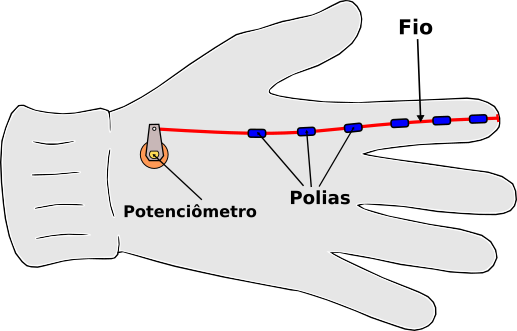
\includegraphics[width=7cm]{./figures/glove-wire-pot1.png}
  		\label{Fig:glove-wire-pot1}
			\fonte{Produzido pelo autor.}
		\end{figure}

			
			\subsection{Componentes eletrônicos}	

			O sistema de processamento e transmissão de sinal da BioGlove foi projetado para ser móvel, leve, alimentado por uma bateria, caber no dorso da mão e ter custo relativamente menor em relação à outras soluções embarcadas com sensores flex. O sistema visa ainda ser de fácil reprodução e permitir adaptações e melhorias por parte de qualquer pessoa com conhecimentos em ferramentas básicas de eletrônica. Por conta dessa motivação, o \textit{hardware} e \textit{software} deste projeto estarão disponíveis gratuitamente na internet. A partir dos objetivos citados, especificamente na parte eletrônica, o primeiro desafio dessa etapa do projeto foi escolher dentre os componentes de fácil acesso no momento, quais deles seriam utilizados para compor a eletrônica presente na placa de circuito impresso que estaria embarcada na luva.
			
			Sendo o potenciômetro o principal componente do transdutor de flexão e o que estaria em maior número na placa (5 no total), este foi o primeiro componente a ser definido. O modelo escolhido deveria ter algumas características para se adequar ao projeto como ser pequeno o suficiente para manter uma distância adequada para outros potenciômetros e componentes, o cursor deveria ser de fácil giro e assim ser acionado com o mínimo de movimento e o grau de rotação total do cursor deveria ser mínimo, porque assim seria possível obter uma maior variação de resistência dado um mesmo grau de giro, visando facilitar a percepção da variação do potenciômetro pelo microcontrolador. 
			
		Inicialmente, só para receber o sinal é preciso conectar diretamente com o microcontrolador um módulo receptor de rádio frequência compatível com o módulo transmissor que está enviando o sinal, em seguida deve-se incluir a biblioteca \textit{VirtualWire} que contém funções para interpretar o sinal recebido. 
			Através da Figura \ref{Fig:pot-comparison} busca-se deixar este último conceito um pouco mais claro. Nesta figura são comparados dois potenciômetros de mesma resistência nominal (8$\,k\Omega$), isto é, ambos os potenciômetros devem apresentar um valor de resistência de 8$\,k\Omega$ quando seus cursores forem totalmente girados. Entretanto, o ângulo máximo de giro dos dois potenciômetros da figura são diferentes entre si, sendo do potenciômetro A = 45º e B = 90º. Por conta desse fato é possível notar que no instante ``1'' da figura, onde ambos estão com 0º de giro, os dois apresentam seu valor de resistência igual a 0$\,\Omega$. Mas no instante ``2'', quando ambos estão com 45º de giro, o potenciômetro A possui resistência de 8$\,k\Omega$ (pois atingiu seu grau máximo), enquanto que o potenciômetro B tem resistência de 4$\,k\Omega$, porque atingiu apenas metade do seu grau de giro máximo característico. Portanto, neste exemplo, o melhor potenciômetro para a BioGlove seria o A porque possui maior variação de resistência por ângulo.

		\begin{figure}[h!]
			\centering
			\caption{Comparação de resistência baseada em ângulo.}
  		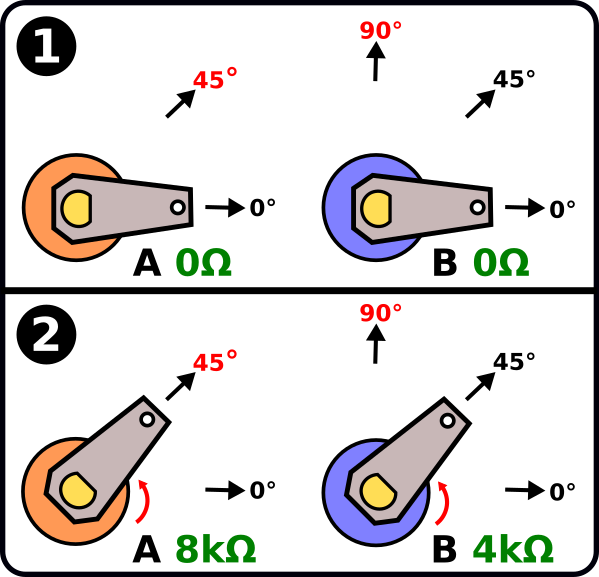
\includegraphics[width=7cm]{./figures/pot-comparison.png}
  		\label{Fig:pot-comparison}
			\fonte{Produzido pelo autor.}
		\end{figure}
			
			O modelo de potenciômetro que mais se aproximou das especificações desejadas foi retirado de servomotores modelo MG996R da marca \textit{TowerPro}. Este potenciômetro possui dimensão aproximada de 13$\,mm$ x 13$\,mm$ em sua base, resistência máxima de 5$\,k\Omega$, giro máximo de $200^{o}$ (aproximado) e seu cursor desliza com facilidade durante o giro. 

			Seguindo adiante com a montagem, para facilitar a instalação do fio de náilon e do elástico no potenciômetro, um pequeno pedaço de PVC (\textit{Polyvinyl Chloride}) expandido foi adaptado no cursor do potenciômetro, objetivando facilitar o giro do cursor durante o uso da luva. O resultado desta adaptação pode ser visto na Figura \ref{Fig:potentiometer-and-battery}(a).

			O componente escolhido para processar os dados recebidos de cada potenciômetro foi a placa Arduino modelo Nano. Isso porque esta placa é leve, ocupa uma área de apenas 45$\,mm$ x 17$\,mm$, possui vasta documentação e disponibilidade no mercado, além de ser compatível com diversos módulos externos e possuir custo menor do que outros modelos da família Arduino.

			Para enviar e receber o sinal de controle da BioGlove, foi escolhido um modelo genérico de um par composto de transmissor e receptor de rádio frequência 433$\,MHz$. Este \textit{hardware} é leve, amplamente disponível no mercado e ainda tem baixo custo se comparado à outras soluções de transmissão de dados sem fio.

			Finalmente, para alimentar todo esse aparato eletrônico, foi escolhida uma pequena bateria LiPo (\textit{Lithium-ion Polymer}) que possui capacidade de 300$\,mAh$, 7,4$\,V$ de tensão nominal e ocupa um espaço de apenas 45$\,mm$ x 12,5$\,mm$ na placa. Este modelo de bateria é mostrado na Figura \ref{Fig:potentiometer-and-battery}(b).


	\begin{figure}[!htb]
		 \centering
		 \caption{ (a) Potenciômetro adaptado e (b) bateria.}
		 \subfloat[]
		 {
			 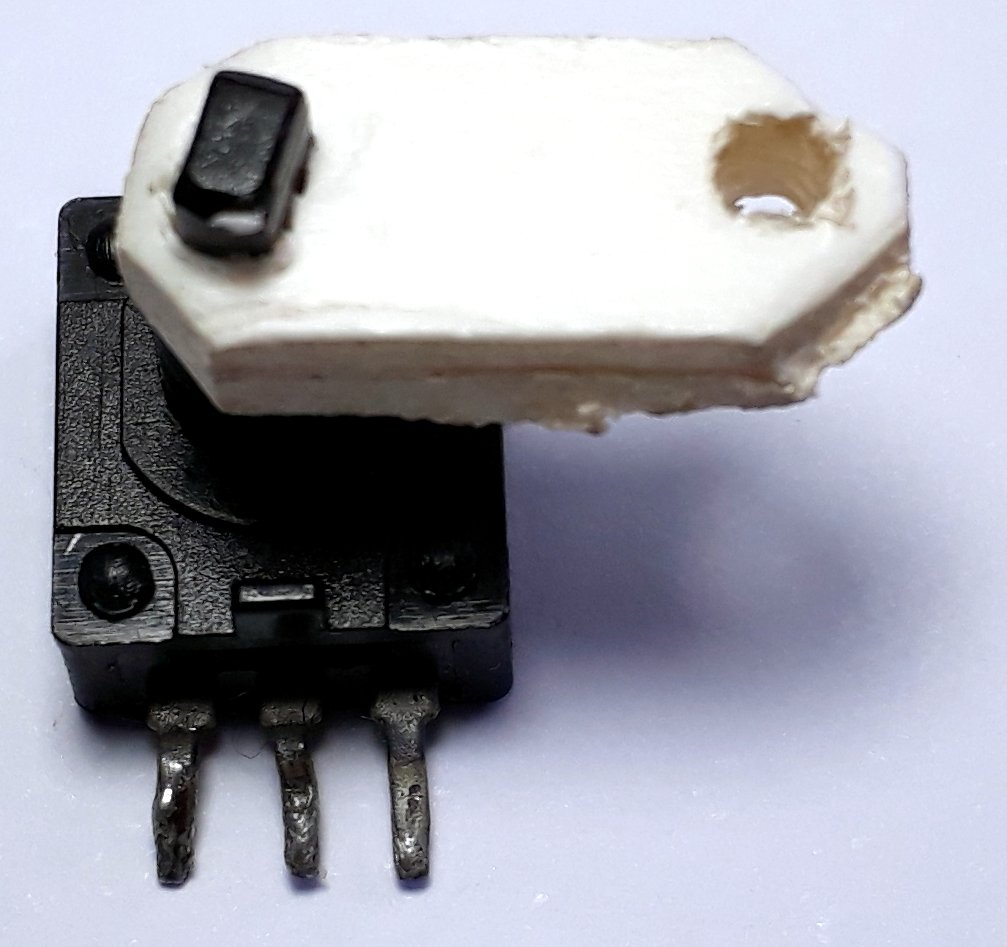
\includegraphics[width=5.5cm,keepaspectratio=true]{./figures/potentiometer3.jpg}
		 }
		 \centering
		 \subfloat[]
		 { 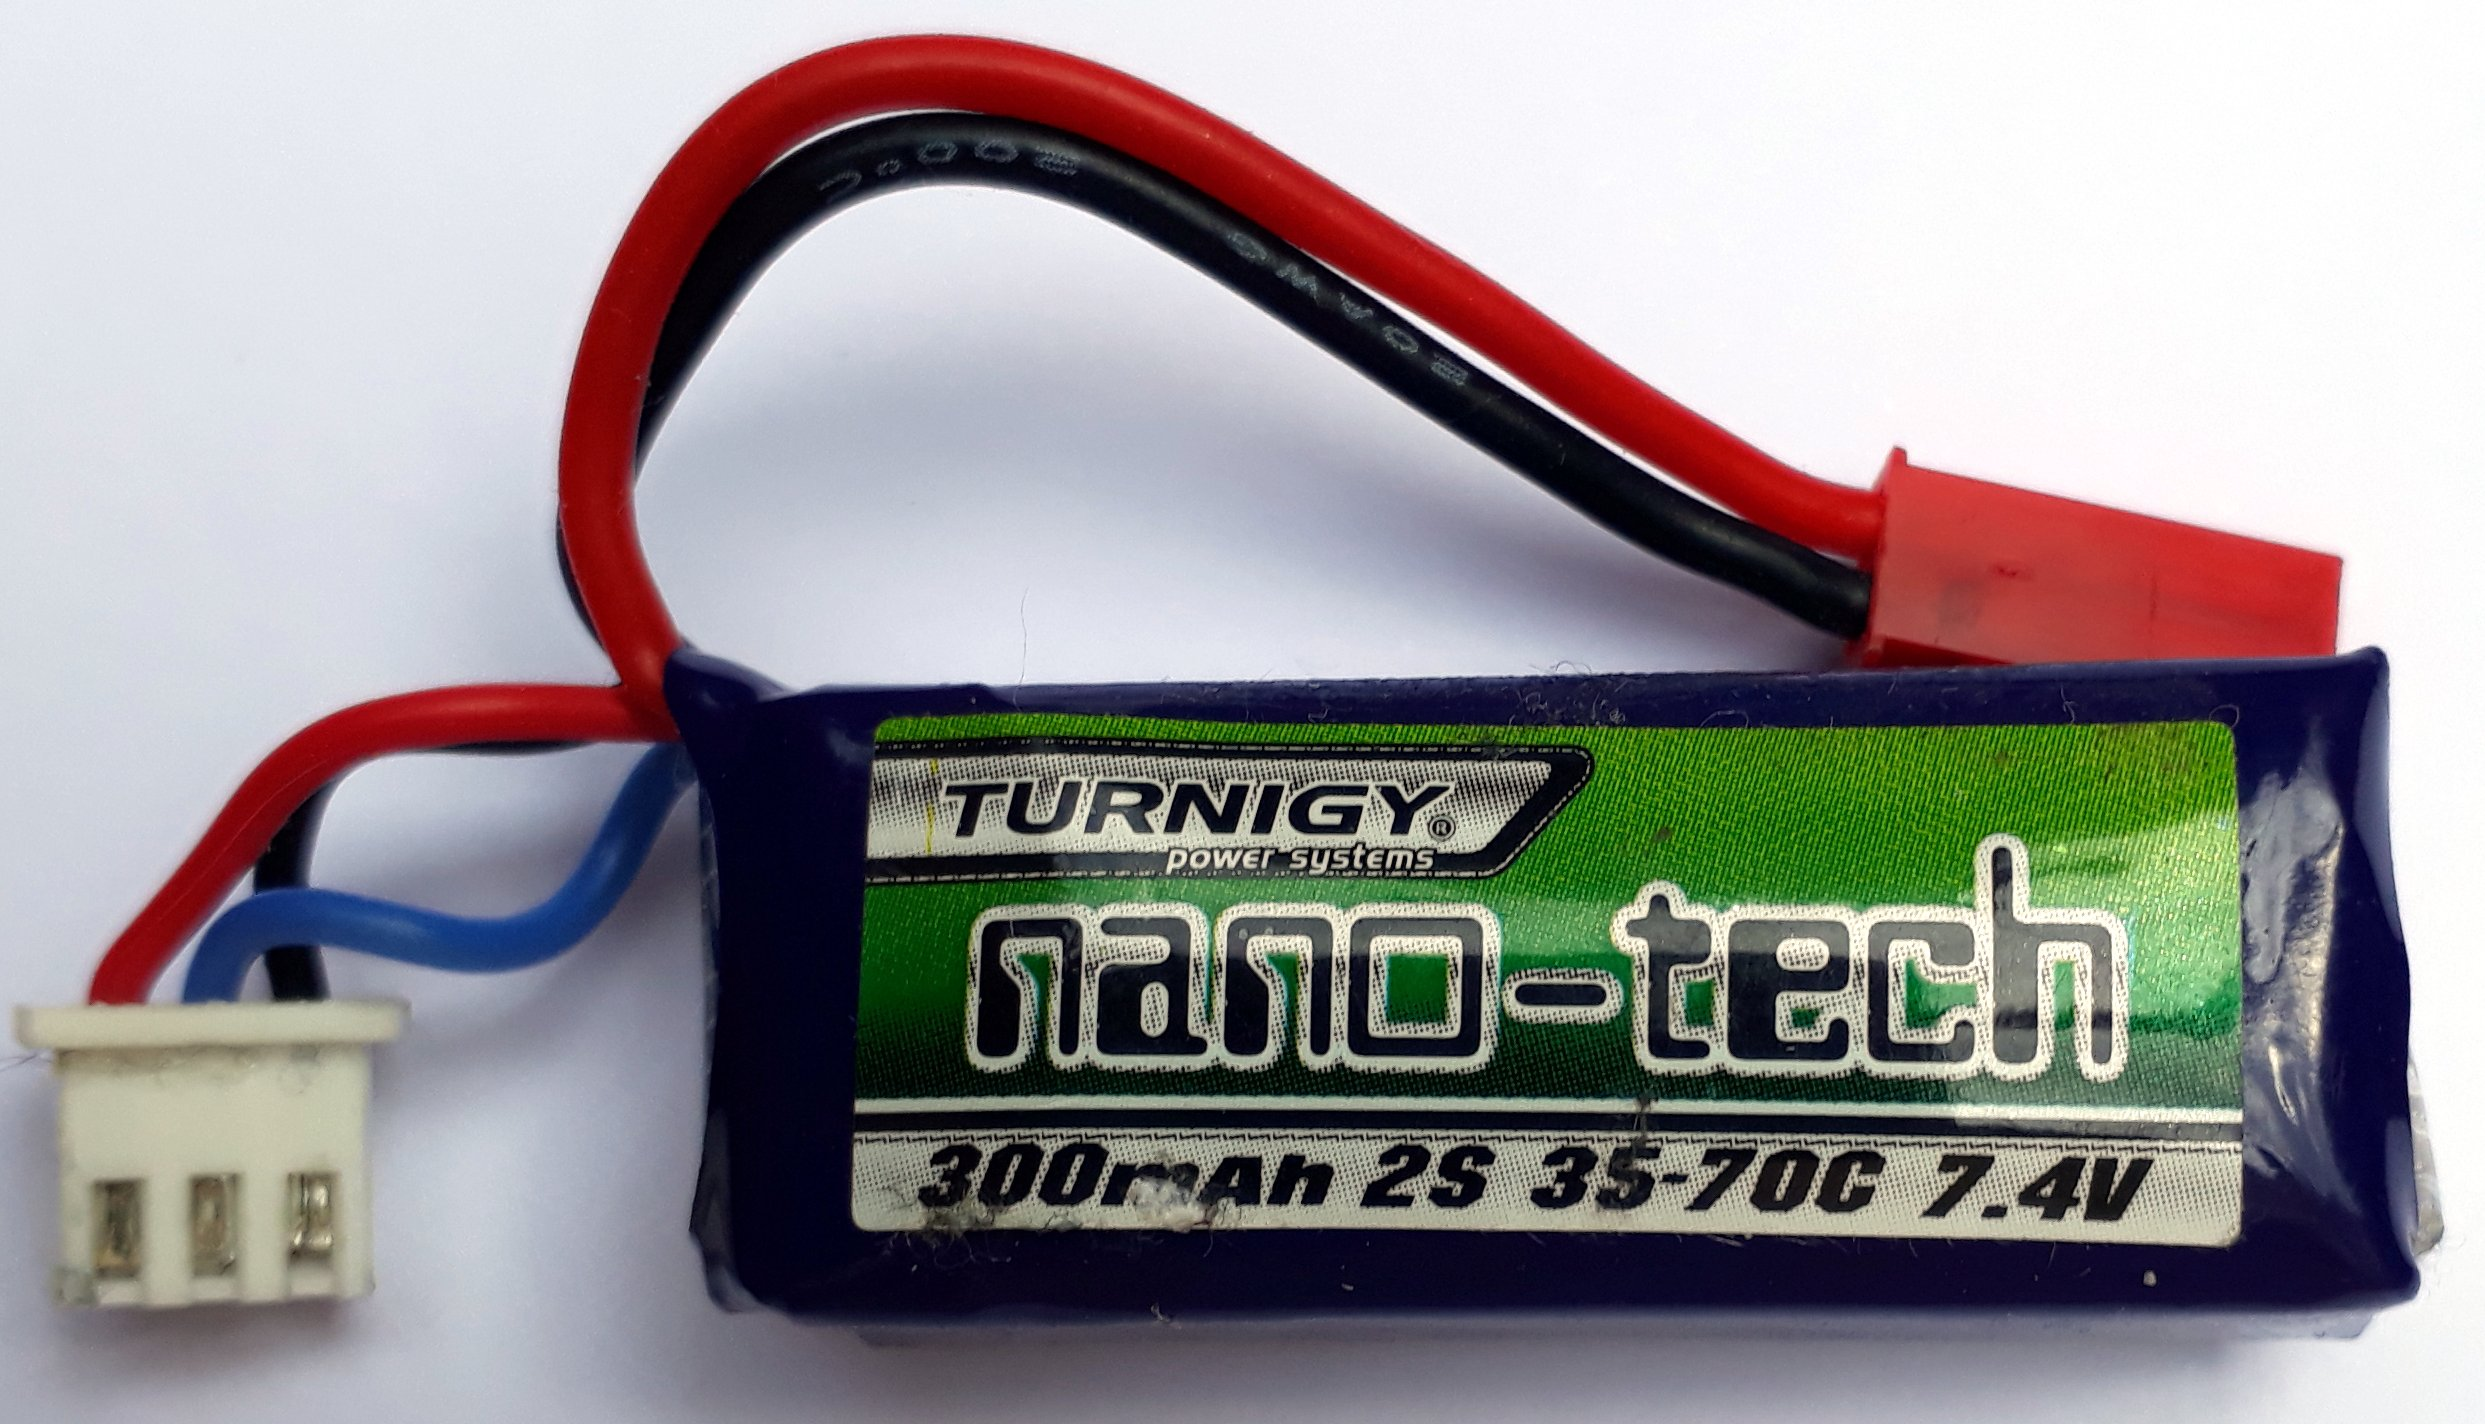
\includegraphics[width=8.5cm,keepaspectratio=true]{./figures/battery1.jpg}
		 }
		 \label{Fig:potentiometer-and-battery}
		 \fonte{Produzido pelo autor.}
	 \end{figure}


			\subsection{Posicionamento de componentes}

			Após definir os componentes que iriam integrar a BioGlove, foram realizadas medições na luva que serviu de modelo para o projeto, e baseado nisso foi decidido que a dimensão máxima da PCI (Placa de Circuito Impresso) que ficaria no dorso da mão deveria ser de aproximadamente 72$\,mm$ x 58$\,mm$. Dessa forma, a placa não ficaria muito maior do que o dorso da luva. 
			
			A partir das dimensões da placa e dos componentes, foi utilizado o \textit{software} QCAD para fazer estimativas a cerca do posicionamento dos componentes na placa, onde todos os potenciômetros deveriam ficar na borda da placa instalada no dorso da mão, alocados o mais próximo possível dos dedos. O microcontrolador deveria estar logo atrás do grupo de potenciômetros por conta das conexões elétricas entre eles. Já o módulo transmissor e a bateria não possuiam recomendações específicas sobre o local de instalação, eles deveriam apenas caber dentro da dimensão máxima da placa. O \textit{layout} desenhado no QCAD pode ser conferido através da Figura \ref{Fig:size-glove-module1}.

		\begin{figure}[h!]
			\centering
			\caption{Alocação dos componentes na PCI.}
  		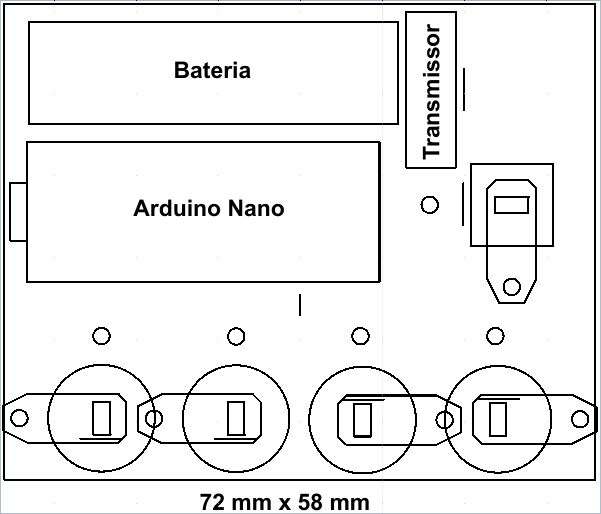
\includegraphics[width=7cm]{figures/size-glove-module1.png}
  		\label{Fig:size-glove-module1}
			\fonte{Produzido pelo autor.}
		\end{figure}


			\subsection{Placa de circuito impresso (PCI)}

			Os primeiros experimentos que definiram o comportamento e as ligações elétricas entre os componentes foram realizados ainda em \textit{protoboard}. Um dos primeiros programas criados lia a variação de um resistor conectado na \textit{protoboard} e mostrava os resultados na tela do computador. Este programa inicial foi evoluindo e com isso mais componentes foram sendo adicionados aos testes de \textit{protoboard}, até o momento em que o \textit{software} foi capaz de controlar todos os componentes do projeto simultaneamente. A partir daí, foi estimado  qual seria a melhor forma de realizar as conexões entre os pinos, potenciômetros, bateria, módulo transmissor e o microcontrolador Arduino em uma PCI de uma camada.

			Para desenvolver a PCI baseada nas ligações da \textit{protoboard}, primeiramente foi dado início ao desenho do esquemático no \textit{software} Kicad, onde foi possível visualizar de forma mais clara todas as conexões elétricas do projeto. Posteriormente, usando o esquemático criado e ainda dentro do Kicad foi possível projetar uma placa de circuito impresso de uma camada posicionando todos os componentes de acordo com as estimativas do QCAD apresentadas na Figura \ref{Fig:size-glove-module1}. Os projetos do esquemático e da PCI realizados através do Kicad estão na Figura \ref{Fig:schematic-and-PCB}.

			Após a conclusão do desenho da placa de circuito impresso, foram efetuados os procedimentos necessários para a transfererência deste desenho para uma placa de fenolite cobreada, e logo depois foi realizada a soldagem de todos os pinos e componentes. A Figura \ref{Fig:phenolic-and-ready} mostra os resultados após o procedimento descrito. 
		
		Com a PCI concluída em mãos, o passo final para a montagem foi conectar os fios de náilon e os elásticos aos cursores dos potenciômetros e costurar a PCI no dorso da luva. A Figura \ref{Fig:glove-ready1} ilustra a montagem completa da BioGlove.

	\begin{figure}[!htb]
		 \centering
		 \caption{ Desenhos projetados no Kicad do (a) esquemático e (b) PCI. }
		 \subfloat[]
		 {
			 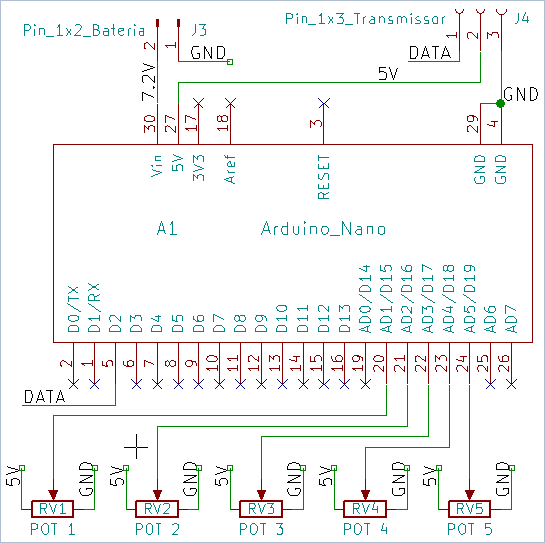
\includegraphics[width=6.5cm,keepaspectratio=true]{./figures/schematic-glove-module1.png}
		 }
		 \centering
		 \subfloat[]
		 { 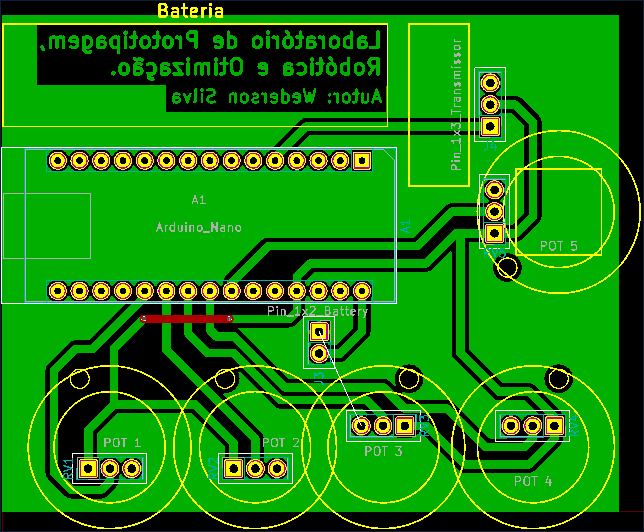
\includegraphics[width=7.5cm,keepaspectratio=true]{./figures/PCB-glove-module1.png}
		 }
		 \label{Fig:schematic-and-PCB}
		 \fonte{Produzido pelo autor.}
	\end{figure}

	
	\begin{figure}[!htb]
		 \centering
		 \caption{(a) Placa de fenolite cobreada e (b) com os componentes soldados.} 
		 \subfloat[]
		 {
			 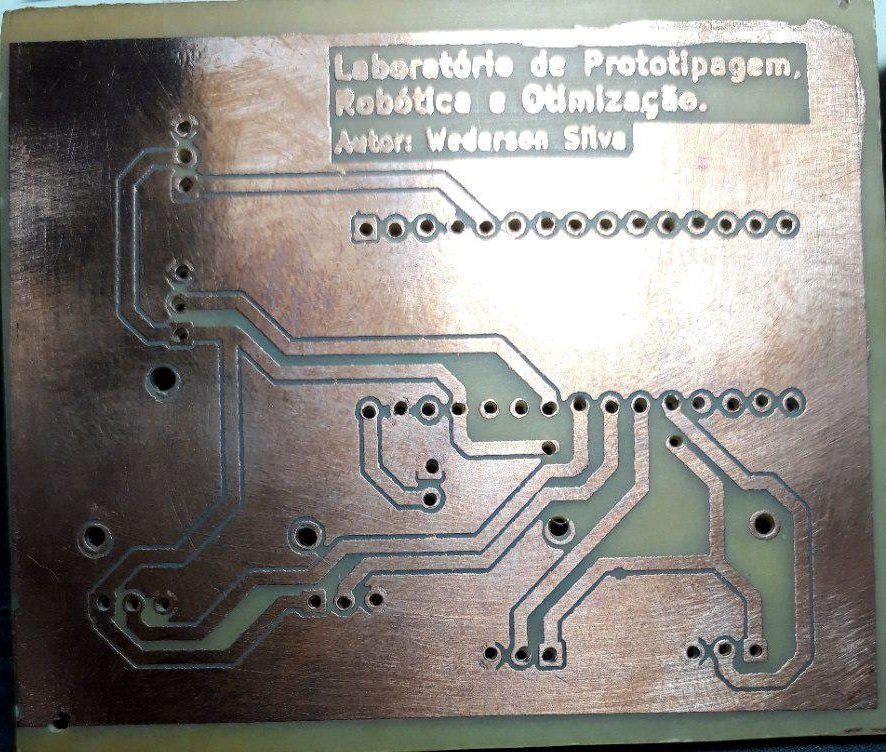
\includegraphics[width=7cm,keepaspectratio=true]{./figures/phenolic-glove-module1.jpg}
		 }
		 \centering
		 \subfloat[]
		 { 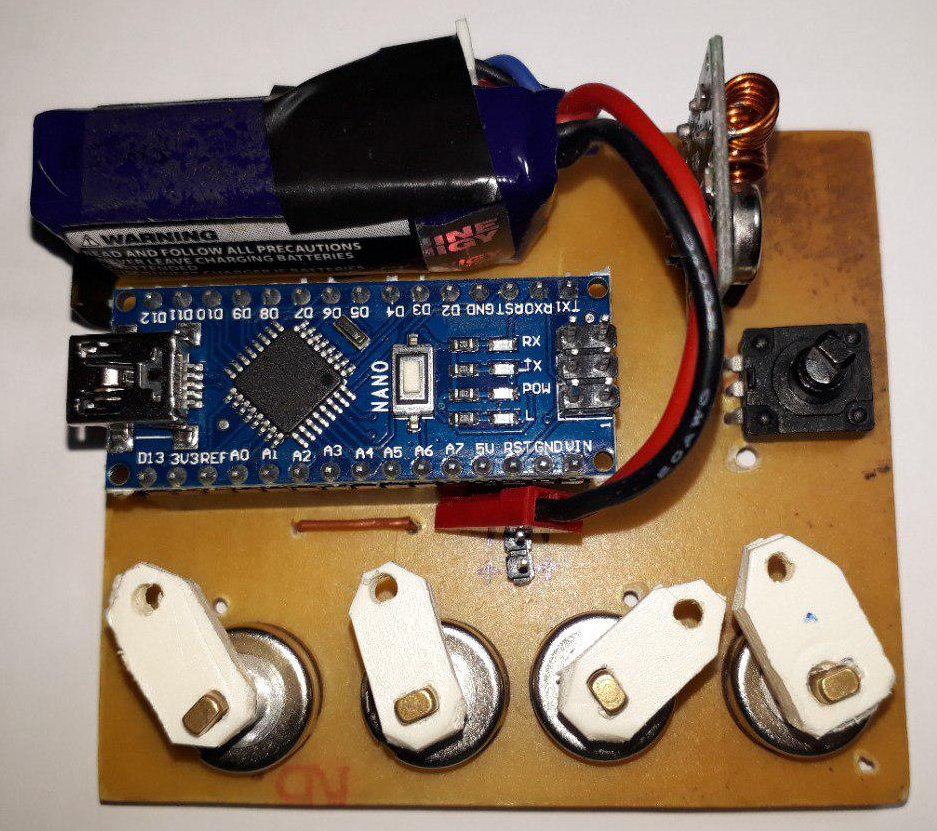
\includegraphics[width=7cm,keepaspectratio=true]{./figures/glove-module-ready1.jpg}
		 }
		 \label{Fig:phenolic-and-ready}
		 \fonte{Produzido pelo autor.}
	\end{figure}

	

		\begin{figure}[h!]
			\centering
			\caption{Protótipo da BioGlove finalizado.}
  		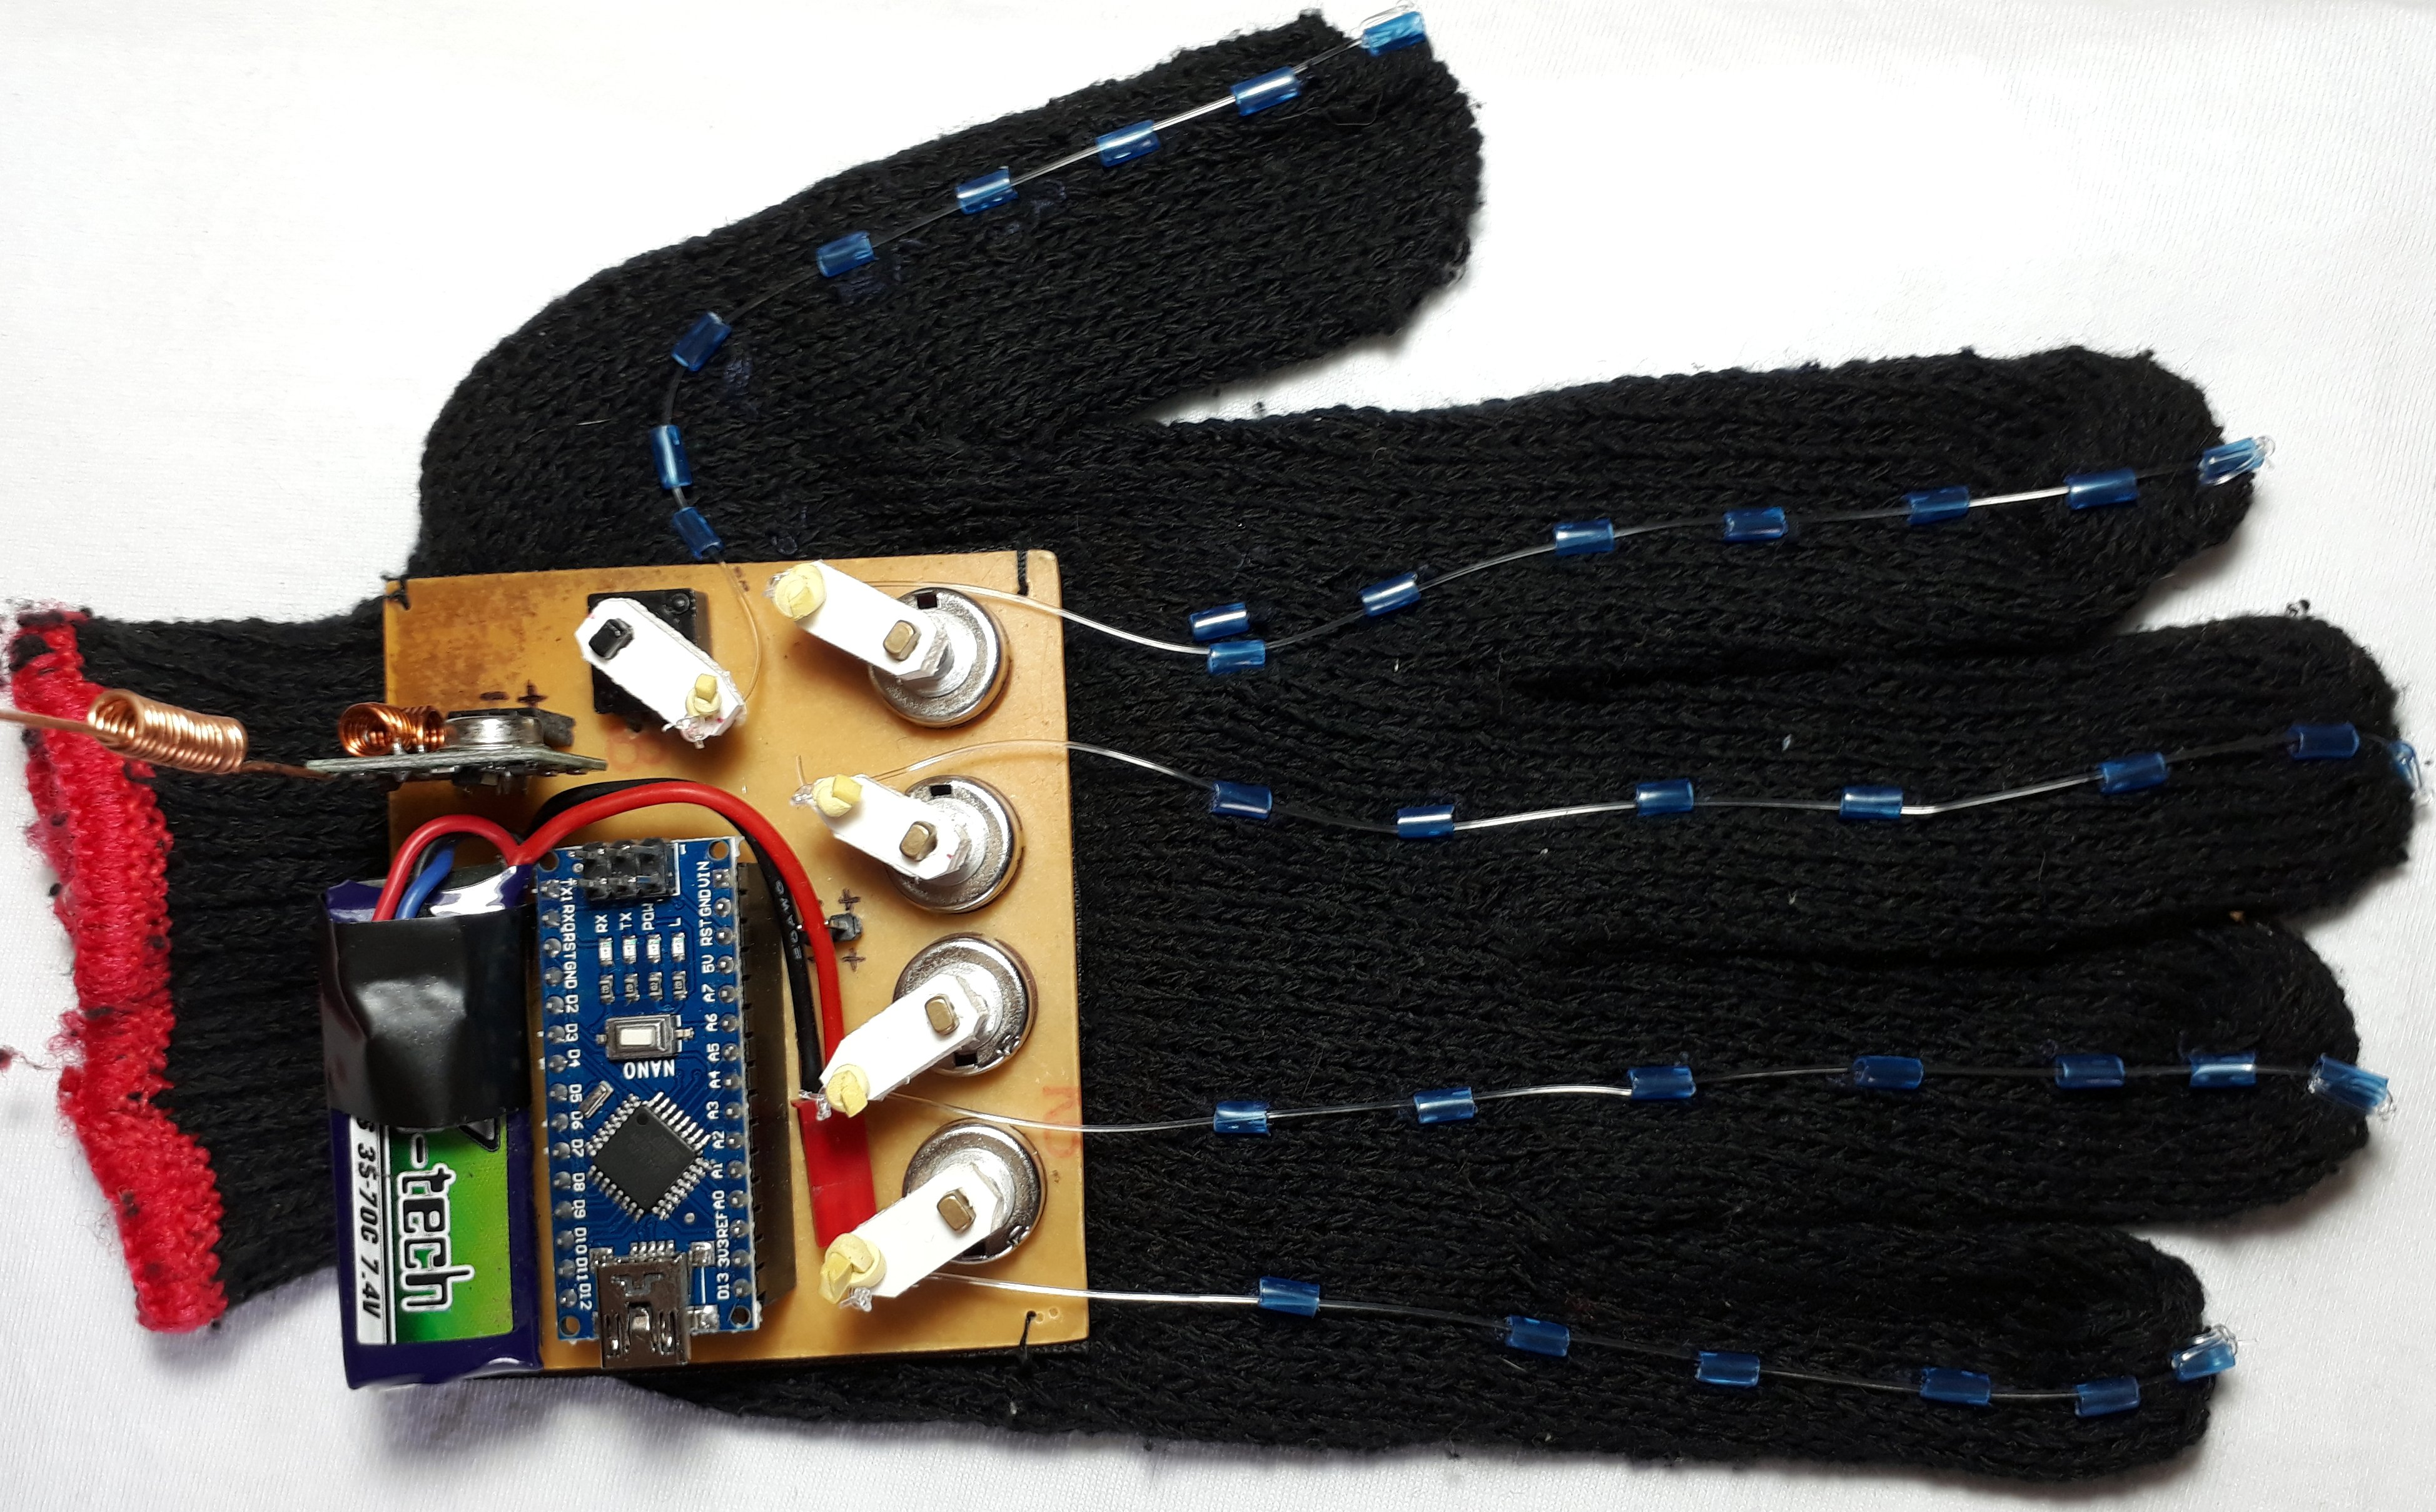
\includegraphics[width=14cm,keepaspectratio=true]{figures/glove-ready1.jpg}
  		\label{Fig:glove-ready1}
			\fonte{Produzido pelo autor.}
		\end{figure}




	% --------------------------------------------------
	%				RESULTADOS E ANÁLISES	
	% --------------------------------------------------


\chapter{Resultados e análises}

		\section{Introdução}
		
		Após a conclusão da montagem da Bioglove, o \textit{software} de transmissão foi carregado para o microcontrolador embarcado nela enquanto que o \textit{software} de recepção de sinal foi carregado no Arduino Nano instalado no carrinho. Além do teste de controle do carrinho em si, outras pesquisas mais aprofundadas a respeito do desempenho da BioGlove foram realizadas. Tais estudos buscaram mensurar alguns dos principais componentes da luva proposta e comparar estes resultados com outros trabalhos envolvendo luvas sensorizadas. As três frentes a serem analisadas são: a sensibilidade do sensor de flexão desenvolvido, a duração do sistema móvel alimentado por bateria e o alcance da transmissão do sinal.
		

		\section{Sensibilidade do sensor de flexão}

		Sendo o sensor de flexão bioinspirado o principal componente da BioGlove, esse teve o seu desempenho mensurado além do controle do carrinho. Como já foi dito, o valor recebido a partir de cada potenciômetro que compõe o sensor de flexão resistivo é digitalizado pelo microcontrolador para uma faixa de 1024 valores possíveis (0 a 1023). Sendo assim, em seu melhor desempenho só seria possível obter no máximo 1024 valores de resolução em cada potenciômetro. Porém, durante o uso da BioGlove entre a posição A (dedos totalmente estendidos) e a posição B (dedos totalmente flexionados) não acontece o giro completo do potenciômetro, sendo assim apenas uma parte dos 1024 valores possíveis é utilizada para detectar os movimentos dos dedos.
		
		O primeiro teste a ser realizado foi o teste de sensibilidade do sistema de detecção de flexão. Sendo este um sensor de flexão, faz-se necessário mensurar a quantidade máxima de posições capturadas em um movimento. Diversos trabalhos utilizam sensores de flexão resistivos comerciais para realizar a captura de movimentos em suas luvas sensorizadas. O desempenho de um desses trabalhos foi utilizado como referência para os testes descritos nesta seção.

		Os sensores de flexão resistivos comerciais, mais conhecidos apenas como sensores flex, são resistores analógicos, e dentro desses sensores existem elementos resistivos de carbono junto a um fino substrato flexível. Quando o substrato é torcido o sensor produz uma resistência relativa ao raio da torção. Quanto maior o raio de torção maior será a resistência apresentada pelo sensor \cite{solanki2013sign}. A Figura \ref{Fig:flex-sensor1} mostra um sensor de flexão resistivo da fabricante Spectra Symbol.

	\begin{figure}[!h]
		\centering
		\caption{Sensor de flexão.}
		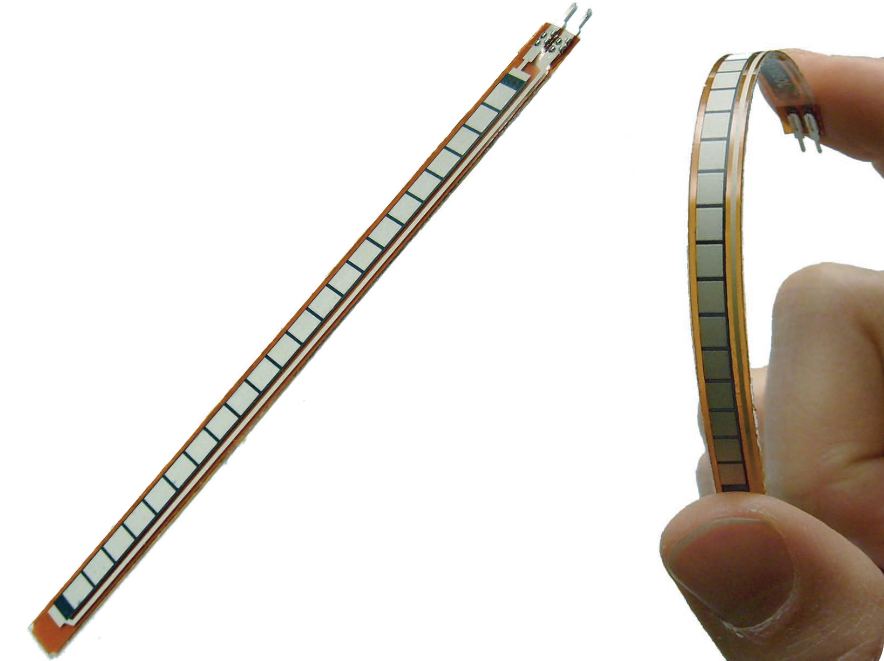
\includegraphics[width=7cm,keepaspectratio=true]{./figures/flex-sensor1.png}
		\fonte{\cite{flexsensor}.}
		\label{Fig:flex-sensor1}
	\end{figure}


		Para demontrar como seria o uso de um sensor de flexão resistivo em um projeto com luva sensorizada, a Figura \ref{Fig:hand-flexsensor-degrees1} apresenta um possível uso do sensor de flexão resistivo comercial posicionado em um dos pontos de flexão do dedo indicador. Além disso, a figura mostra o que seriam os graus de torção deste sensor. À esquerda estão a mão e o sensor (em azul), em posição inicial, ambos com ângulo de flexão de aproximadamente 0 (zero) grau. À direita está o resultado de um movimento de flexão de aproximadamente 90 graus em relação à posição anterior.


	\begin{figure}[!h]
		\centering
		\caption{Sensor de flexão resistivo comercial na mão durante a flexão.}
		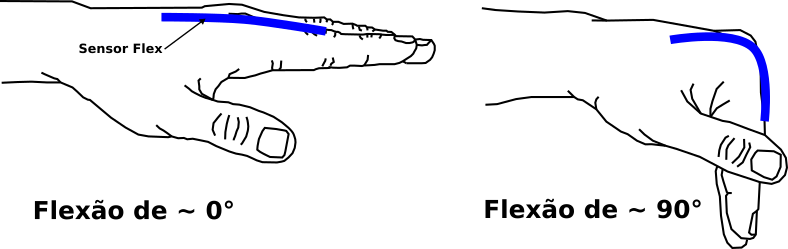
\includegraphics[width=13cm,keepaspectratio=true]{./figures/hand-flexsensor-degrees1.png}
		\fonte{Produzido pelo autor.}
		\label{Fig:hand-flexsensor-degrees1}
	\end{figure}

	
		O trabalho de \cite{anbarasi2013deafmute}, que será utilizado como referência, utiliza sensores de flexão resistivos comerciais de 2,5 e 4,5 polegadas. Sobre o desempenho do dos sensores de flexão resistivos de sua aplicação, o autor cita que durante os testes, os sensores de flexão resistivos de 2,5 polegadas foram instalados nos dedos mínimo e polegar, enquanto que os sensores de 4,5 polegadas foram instalados nos dedos indicador, médio e anelar. Em sua publicação, ele apresenta valores obtidos por cada sensor nas posições de flexão de 0 graus e 90 graus. Para efeitos de comparação, através da BioGlove também foram realizados movimentos relativos às flexões de 0 e 90 graus. 
		
		Seguidamente, as equações (\ref{Eq:Desloca1}) e (\ref{Eq:NPos1}) serviram de referência para calcular a resolução (ou sensibilidade) de cada sistema. Sendo que, para os cálculos deste teste PosB recebe o valor digital em 90 graus e PosA recebe o valor digital em 0 grau. Portanto, os valores digitais relativos às mesmas posições em ambos os trabalhos foram utilizados como entrada das equações: 
		
	\begin{equation}
			\Delta Pos 	= Pos 90 	- 	Pos 0
		\label{Eq:Desloca2}
	\end{equation}


	\begin{equation}
			NPos = |\Delta Pos| + 1 .
		\label{Eq:NPos2}
	\end{equation}


		A Tabela \ref{Tab:NPos0-90} reúne os valores obtidos em 0 grau (Pos0), 90 graus (Pos90) e o número de posições possíveis (NPos) ou sensibilidade calculados através de (\ref{Eq:Desloca2}) e (\ref{Eq:NPos2}) referentes aos sensores de flexão comercial e aos sensores bioinspirados da BioGlove. O dedo polegar não está presente na tabela porque ele não é flexionado durante o movimento realizado neste teste.
		
%		\begin{table}[H]
%  	\centering
%		\caption{Valores obtidos e número de posições entre 0 e 90 graus dos sensores de flexão.}
%    \begin{tabular}{l|ccccccc}
%      \midrule
%			Posições&\textcolor{red}{2,5''}	&\textcolor{red}{4,5''}	& Minimo	& Anelar	& Médio	&	Indicador	\\
%      \midrule
%			Pos0 		& 748 									& 350 									& 206 		&	142			&	771		&	746				\\
%			Pos90 	& 875 									& 568 									& 309 		&	396			&	527		&	607				\\
%			NPos 		& 128 									& 219 									& 104 		&	255			&	245		&	140				\\
%      \midrule
%    \end{tabular}
%		\label{Tab:NPos0-90}
%    \fonte{Adaptado de \cite{anbarasi2013deafmute} e produzido pelo autor.}
%		\end{table}


\begin{table}[H]
	\centering	
	\caption{Valores obtidos e número de posições entre 0 e 90 graus dos sensores de flexão.}
		\begin{tabular}{c|cc|cccc} 
			\midrule
\multirow{2}{*}{Posições} & \multicolumn{2}{c|}{\textbf{Comercial}} & \multicolumn{4}{c}{\textbf{Bioinspirado - BioGlove}}\\
			    		& 2,5'' 	& 4,5'' 	& Mínimo 	& Anelar 	& Médio & Indicador \\
		  \midrule
			Pos0 		& 748 		& 350 		& 206 		&	142			&	771		&	746				\\
			Pos90 	& 875 		& 568 		& 309 		&	396			&	527		&	607				\\
			NPos 		& 128 		& 219 		& 104 		&	255			&	245		&	140				\\
		  \midrule
		\end{tabular}
	\label{Tab:NPos0-90}	
  \fonte{Adaptado de \cite{anbarasi2013deafmute} e produzido pelo autor.}
\end{table}

		Através da Tabela \ref{Tab:NPos0-90} é possível notar que no quesito sensibilidade, o maior número de posições detectáveis (NPos) foi apresentado pelo dedo anelar da BioGlove, já a menor sensibilidade ficou por conta do dedo mínimo também da BioGlove. Os demais resultados mostram que o sensor de flexão resistivo comercial de 4,5 polegadas apresenta desempenho superior aos dedos indicador e mínimo da BioGlove, enquanto que o modelo comercial de 2,5 polegadas apresenta baixo desempenho em quase todos os casos, exceto quando comparado ao dedo mínimo da BioGlove.

		Com base no desempenho geral apresentado pela Tabela \ref{Tab:NPos0-90}, verifica-se que usando o sensor bioinspirado que compõe a BioGlove, os sensores dos dedos anelar e médio apresentaram os melhores desempenhos mesmo quando comparados ao sensor de flexão resistivo comercial de 4,5 polegadas. Além do mais, 3 dos 4 sensores da BioGlove possuíram desempenho superior se comparados apenas ao sensor de flexão resistivo comercial de 2,5 polegadas. Dessa forma é possível afirmar que os sensores bioinspirados da BioGlove conseguiram desempenho equiparado ao de um sensor comercial. Sendo que um sensor de flexão resistivo comercial possui um custo relativamente superior.


			\section{Autonomia do sistema}

			Mobilidade é um dos requisitos do projeto da BioGlove. Por conta desse fato, foi decidido que a alimentação dos componentes eletrônicos da luva seria feita através de uma pequena bateria LiPo. Outros sistemas envolvendo luvas sensorizadas móveis também costumam usar baterias ou até mesmo pilhas, sendo que o desempenho de cada projeto neste quesito pode variar de acordo com o \textit{hardware} implementado e a capacidade da fonte de alimentação escolhida. Nesta seção, apresentam-se testes de desempenho da bateria da Bioglove que foram comparados com outros dois trabalhos relacionados com luvas sensorizadas.

			O \textit{hardware} da Bioglove está equipado com cinco potenciômetros, um microcontrolador Arduino modelo Nano, um módulo transmissor de rádio frequência 433$\,MHz$ e uma bateria LiPo recarregável de tensão nominal de 7,4$\,V$ e capacidade de 300$\,mAh$, segundo o fabricante. Esta bateria apesar de possuir tensão nominal de 7,4$\,V$, consegue alcançar níveis de tensão de até 8,4$\,V$ quando está totalmente carregada \cite{buchmann2016batteries}.

			Esse modelo de bateria foi escolhido por conta de sua disponibilidade, peso e por ser compatível com as recomendação para alimentar o Arduino Nano, que deve estar com tensões entre 7$\,V$ e 12$\,V$ segundo \cite{arduinopowerrange}. Por conta desse fato, a BioGlove funciona normalmente com a bateria carregada até o momento em que a tensão da bateria descarrega no limite de 7$\,V$. Caso a bateria não seja substituída e continue a ser usada na BioGlove, a partir desse ponto de tensão o microcontrolador passa a reiniciar constantemente impossibilitando o uso da BioGlove até que a bateria seja recarregada ou substituída.

			Para realizar os testes de desempenho da bateria da BioGlove, um módulo receptor compatível com o transmissor da luva foi conectado a um Arduino programado para receber os sinais transmitidos pela luva. Este Arduino foi conectado a um computador que mostrava em sua tela as mensagens recebidas da BioGlove. Além disso, uma bateria recém carregada completamente foi conectada à luva e o momento inicial da ligação do sistema foi marcado. Durante o teste, o módulo transmissor da luva ficou ligado constantemente, enviando mensagens a todo momento. E a cada período de tempo regular, a tensão da bateria foi sendo monitorada. Este teste foi realizado quatro vezes no total, usando duas baterias de mesmo modelo, duas vezes para cada bateria. Com isso, obteve-se um período de duração de aproximadamente 10 horas onde, em média, a tensão da bateria chegava ao limite definido de 7$\,V$.

%			Dentre as aplicações que foram comparadas à BioGlove está a luva comercial chamada Data Glove 5 Ultra da fabricante 5DT Inc., que foi desenvolvida, entre outras funcionalidades, para ser utilizada em modelagem 3D e animação através de programas de computador compatíveis com ela. De acordo com o seu \textit{datasheet}, a Data Glove 5 Ultra possui em seu \textit{hardware} sensores de flexão baseados em fibra óptica, utiliza tecnologia de comunição sem fio Bluetooth, além afirmar que o desempenho de sua bateria recarregável pode chegar a 8 horas de duração \cite{5DT-ultra}. Entretanto, por ser um produto comercial fechado, não foi possível obter informações sobre a tecnologia de sua bateria.

			Uma das aplicações comparadas à BioGlove foi a pesquisa de \cite{michela2013rehab} que busca através de uma luva sensorizada, mensurar a flexão dos dedos para estudos de reabilitação. O \textit{hardware} desta luva é embarcado com sensores de flexão resistivos comerciais, um microcontrolador e um transmissor de rádio frequência. Sendo que toda a eletrônica do projeto é alimentada por uma bateria em formato de botão que possui tensão nominal de 3$\,V$ e capacidade de 1000$\,mAh$. De acordo com o artigo publicado, sua luva sensorizada obteve uma duração aproximada de uma semana.
			
			O último trabalho a ser comparado é o de uma luva de baixo custo que foi desenvolvida na pesquisa de \cite{simone2007lowcost} com o propósito de monitorar a flexão dos dedos de pessoas com disfunções na mão. De acordo com o autor, o \textit{hardware} dessa luva é composto por sensores de flexão resistivos comerciais e uma placa embarcada com um microprocessador, uma memória RAM externa, um transmissor de sinal padrão IEEE 802.15.4, além de pilhas AA alcalinas. Segundo a publicação deste estudo, usando duas pilhas novas durante os testes, o sistema conseguiu ser alimentado por quase 60 horas. Infelizmente a capacidade destas pilhas não foi definida no trabalho publicado, porém \cite{buchmann2016batteries} cita que esse tipo de pilha possui capacidade de até 2870$\,mAh$ e tensão de 1,5$\,V$ cada.
			

			De forma geral e focado apenas nas características das fontes de alimentação apresentadas até o momento, a Tabela \ref{Tab:battery-range} resume o desempenho dos trabalhos discutidos nesta seção.

		\begin{table}[H]
  	\centering
		\caption{Desempenho de alimentação das luvas.}
    \begin{tabular}{c|c|c|c}
      \midrule
			Luva 								& Alimentação							&	Capacidade	& Duração	\\
      \midrule                                            					
			Luva sensorizada 		& 1 bateria-botão	3$\,V$	& 1000$\,mAh$		& 1 semana\\
			Luva de baixo custo & 2 pilhas AA 3$\,V$			& 5740$\,mAh$		& 60 horas\\
			BioGlove						& 1 LiPo 7,4$\,V$					& 300$\,mAh$			&	10 horas\\	
      \midrule
    \end{tabular}
		\label{Tab:battery-range}
    \fonte{Produzido pelo autor.}
		\end{table}

		Analisando a Tabela \ref{Tab:battery-range}, percebe-se que a luva sensorizada alimentada por bateria-botão possui o melhor desempenho dentre todos os analisados, pois 1 semana de duração é quase três vezes a duração do segundo colocado, isso pode ser atribuído principalmente ao \textit{hardware} de baixo consumo de energia embarcado e ao número reduzido de componentes que compõe o projeto de \cite{michela2013rehab}. A luva de baixo custo desenvolvida em \cite{simone2007lowcost} também apresenta um desempenho excepcional, seis vezes maior do que a BioGlove, e que pode ser atribuído pela alta capacidade fornecida através das 2 pilhas alcalinas que alimentam o sistema.

%		A luva Data Glove 5, apesar de ser um produto comercial, possui o pior desempenho dentre todos os analisados, além disso o \textit{hardware} fechado dificulta a análise para além da duração de sua bateria. Porém, deve-se notar que esta luva oferece diversos recursos ao usuário como calibração, compatibilidade com diversos sistemas operacionais e \textit{softwares} \cite{5DT-ultra}. Portanto, seu elevado consumo de energia  pode ser caracterizado pela provável complexidade e quantidade de \textit{hardware} inclusos neste produto.

		A BioGlove acabou tendo o segundo pior desempenho comparando com as outras luvas. Sua alimentação de baixa capacidade, o uso de uma placa comercial pronta recheada de componentes e o envio constante de mensagens através de seu módulo transmissor podem ser as principais causas desse curto período de duração apresentado. Entretanto, pelo fato de a placa embarcada usar um Arduino, esta placa também pode ser alimentada via cabo USB, o que viabilizaria projetos que não tem a mobilidade como foco princiapal, e nesse caso a BioGlove poderia ser usada sem preocupações quanto a duração de sua bateria pois estaria conectada constantemente à fonte de energia do cabo USB.

			\section{Alcance da comunicação sem fio}

		Em projetos móveis relacionados com luvas sensorizadas e que usam transmissão de dados sem fio, o alcance da comunicação entre o emissor e o receptor é limitado pela tecnologia empregada nesses equipamentos. \textit{Hardwares} com maior potência alcançam maiores distâncias, mas costumam ter um custo mais elevado. Porém, existem tecnologias de transmissão de baixo custo e de menor potência como a que foi empregada na BioGlove. 
			
		Dentre as diversas opções para se implementar comunicação sem fio, existem projetos que utilizam transmissão via \textit{Bluetooth}, que viabiliza a interação com computadores, \textit{smartphones} ou qualquer outro dispositivo compatível que esteja próximo. Outros projetos chegam a usar a tecnologia de rede Wi-Fi e com isso são capazes de enviar comandos através da internet, podendo interagir com qualquer dispositivo conectado à grande rede mundial. Na seção a seguir, o alcance de dois projetos relacionados à luvas sensorizadas e que utilizam a tecnologia \textit{Bluetooth} serão comparados ao método de transmissão via rádio de baixa frequência utilizado na BioGlove.

		A BioGlove está equipada com um par de módulos genéricos para transmissão e recepção de rádio frequência que trabalham na faixa de 433$\,MHz$. De acordo com o manual da biblioteca \textit{VirtualWire} que auxilia o uso desses dispositivos, ao instalar uma antena de cerca de 17$\,cm$ em ambos os módulos o alcance de transmissão pode ser de até 150 metros em campo aberto \cite{virtualwiremanual}. Entretanto, neste trabalho, por conta da fragilidade de um dos módulos, só foi possível soldar uma antena no transmissor de rádio, deixando o receptor sem a sua antena o que pode vir a comprometer o desempenho.

		O primeiro teste de alcance foi realizado diretamente com o carrinho e serviu apenas para verificar se o carrinho obedecia aos comandos da luva. Logo nos primeiros testes de controle do carrinho, ele correspondeu aos comandos de movimentação programados na maioria das vezes em que foi testado, porém em alguns momentos haviam atrasos anormais entre o gesto efetuado na luva e o tempo de resposta do carrinho ao comando, estes atrasos se tornavam cada vez mais frequentes à medida que o carrinho se aproximava do limite da área de alcance do transmissor, até o momento em que o carrinho parava totalmente de responder.

		Para realizar o segundo teste de alcance, um módulo receptor foi conectado a uma placa Arduino que por sua vez foi conectada a um computador, sendo assim o equipamento responsável por receber o sinal ficou fixo em um local. Na tela do computador eram exibidas as mensagens enviadas pela BioGlove. Partindo de uma distância igual a zero, o transmissor embarcado na luva foi sendo distanciado aos poucos em campo aberto do receptor, enquanto isso, as mensagens capturadas pelo receptor foram constantemente verificadas na tela do computador. Ao se distanciar por volta de 7,5 metros o sinal da BioGlove começou a falhar e o teste foi encerrado nesta marca. 

			O próximo sistema que foi verificado para efeitos de comparação foi o \textit{Data Glove} 5 \textit{Ultra}, que em seu datasheet oferece informações sobre sua tecnologia de transmissão sem fio. Nele está especificado que atrelado à essa luva comercial existe um kit de transmissão sem fio, no qual foi projetado para suportar até duas luvas simultaneamente. A tecnologia de transmissão utilizada é a \textit{Bluetooth}, que trabalha na faixa de 2,4$\,GHz$ e segundo a sua documentação consegue um alcance de até 20 metros \cite{5DT-ultra}.

			E por fim, foi analisada a PERCRO \textit{Dataglove} que é uma luva baseada no funcionamento de goniômetros, que são instrumentos responsáveis por medir o deslocamento angular relativo. Esta luva sensorizada foi desenvolvida no trabalho de \cite{rodriguez2007goniometric}, e possui dois sensores para cada dedo, um microcontrolador embarcado e um módulo \textit{Bluetooth} 2,4$\,GHz$ que segundo a publicação chega a alcançar uma comunicação satisfatória a uma distância de até 10 metros.


			A Tabela \ref{Tab:wifi-range} abaixo resume o desempenho de alcance apresentado pelas três luvas descritas.

		\begin{table}[H]
  	\centering
		\caption{Desempenho de alcance das luvas.}
    \begin{tabular}{c|c|c|c}
      \midrule
			Luva 						& Tecnologia			&	Faixa		& Alcance		\\
      \midrule                                            					
			\textit{Data Glove} 5			& \textit{Bluetooth}				& 2,4$\,GHz$	& 20 metros	\\
			PERCRO \textit{Dataglove}	& \textit{Bluetooth}				& 2,4$\,GHz$	& 10 metros	\\
			BioGlove				& Rádio Frequência& 433$\,MHz$	&	7,5 metros\\	
      \midrule
    \end{tabular}
		\label{Tab:wifi-range}
    \fonte{Produzido pelo autor.}
		\end{table}

			Observa-se pela Tabela \ref{Tab:wifi-range} que apesar de duas luvas usarem a mesma tecnologia, apresentam resultados diferentes entre si. Isso pode ser atribuído à diferentes versões dos módulos utilizadas ou à potência empregada em cada módulo. A luva comercial \textit{Data Glove} 5 demonstrou o melhor desempenho chegando a ter o dobro do alcance útil de tranmissão em relação à PERCRO \textit{Dataglove}.

			O pior desempenho de alcance ficou por conta da BioGlove que emprega uma tecnologia de comunicação mais barata e diferente das demais, apresentou um desempenho muito inferior ao indicado no manual. Isso pode ser atribuído à aparente baixa qualidade dos componentes utilizados e a ausência de antena no módulo receptor. Entretanto, a BioGlove conseguiu um alcance relativamente próximo ao da PERCRO \textit{Dataglove}. A substituição dos módulos ou a instalação de melhores antenas em ambos os módulos talvez contribua para um melhor desempenho de transmissão futuramente.


	% ----------------------------------------
	%							CONCLUSÃO	
	% ----------------------------------------



		\chapter{Conclusão e trabalhos futuros}
		
		Este trabalho apresentou o desenvolvimento de uma luva de uso geral que possui sensores de flexão bioinspirados embarcados. Além dos sensores, a BioGlove conta com um microcontrador responsável por captar e processar sinais recebidos, um protocolo de comunicação e controle simplificado, e um transmissor de sinal sem fio. A aplicação escolhida para demonstrar a funcionalidade desse sistema foi o controle sem fio de um carrinho eletrônico. Ademais, a avaliação da BioGlove se concentrou em três aspectos principais: o nível de sensibilidade do sensor de flexão proposto; a autonomia do sistema de alimentação; e o alcance da comunicação sem fio.

		Com relação a autonomia da luva, a bateria LiPo recarregável utilizada na BioGlove possui a menor capacidade e apresentou um desempenho relativamente curto durante o uso ininterrupto frente à outros sistemas. Entretanto, o uso de uma fonte de energia com capacidade semelhante às das outras luvas elevaria o desempenho energético da BioGlove. Com relação ao alcance da comunicação sem fio, a BioGlove utilizou módulos de comunicação 433$Mhz$, e apresentou o pior desempenho quando foi comparado às outras soluções que usam a technologia \textit{Bluetooth}. Mas, pelo fato de que a comparação foi feita entre technologias diferentes, fica o questionamento se a BioGlove conseguiria desempenho semelhante às outras luvas caso também usasse módulos \textit{Bluetooth}.


		Baseado nos resultados apresentados, este trabalho se mostrou viável em comparação à outras soluções semelhantes, mesmo frente à um produto comercial. Em alguns aspectos avaliados nos testes, a BioGlove conseguiu se equiparar à outros projetos. Com relação ao foco da pesquisa da luva, o sensoriamento de flexão, a BioGlove chegou até mesmo a ser superior ao sensor de flexão resistivo comercial que é um produto amplamente utilizado em diversos projetos. A partir dos resultados também é possível perceber que pequenas mudanças podem influenciar na melhoria do desempenho em futuros testes. A vida útil da luva pode ser melhorado pelo uso de uma bateria mais potente e pelo aperfeiçoamento da forma de transmissão de mensagens, enviar apenas quando for necessário, e não a todo momento como acontece atualmente. A inclusão de antenas melhores em ambos os módulos de rádio frequência ou a troca da tecnologia de transmissão, por \textit{Bluetooth} por exemplo, pode garantir uma melhoria no alcance de transmissão.

		Neste trabalho, os maiores desafios se apresentaram durante a escolha de componentes e montagem da luva. Por ainda não haver muitas referências de trabalhos com mecânica semelhante, durante a construção, os problemas inesperados foram sendo resolvidos com uso de componentes e ferramentas disponíveis no momento, mesmo que esses não fossem os ideais. Portanto, a troca de componentes por outros mais precisos, menores e que consumam menos energia, podem garantir ainda melhorias na estabilidade da luva.

		Os protocolos de comunicação e controle criados, mesmo sendo simples, alcançaram satisfatoriamente ao seu objetivo inicial de controlar os movimentos do carrinho dentro do raio de alcance do transmissor. Dessa forma os mesmos protocolos ou outros semelhentes tem a possibilidade de serem aproveitados em outras aplicações de transmissão e controle. Entretanto, para aplicações mais complexas ou que exijam uma demanda maior dados durante a transmissão, ao invés de apenas 5 \textit{bytes} por mensagem, será necessária uma melhoria no protocolo de comunicação ou até mesmo a substituição do mesmo.

		Este protótipo foi desenvolvido, usado e testado por apenas uma pessoa. O uso da luva por outras pessoas pode apresentar resultados diferentes e necessitar de ajustes. Cada pessoa possui características diferentes em suas mãos, dedos maiores ou menores, mão mais larga ou mais fina, diferentes graus de flexão dos dedos, entre outros. Portanto, a inclusão de uma função de calibração automática no \textit{software} de transmissão se faz necessária e pode diminuir maiores contratempos quando a BioGlove for utilizada por outros indivíduos.

		Apesar de no geral o projeto desenvolvido se mostrar viável para ser uma luva de aferição de movimentos e transmissão de dados, este possui natureza diferente de outros produtos semelhantes. Enquanto que o uso de sensores de flexão resistivos comerciais pode trazer uma mecânica relativamente estável durante os movimentos, a BioGlove é dependente de uma rede de fios e polias que não apresentaram muita estabilidade mecânica em uma luva de algodão. A troca do material da luva por um  mais rígido, poderia favorecer a estabilidade durante os movimentos.

		A BioGlove, mesmo apresentando limitações, se mostra capaz de fomentar projetos de baixo custo que necessitem desse tipo de equipamento. O uso de componentes de baixo custo, como potenciômetros e o par de comunicação em rádio frequência de 433$\,MHz$, além da conhecida placa Arduino permite, com os devidos ajustes, que diversos módulos compatíveis sejam adicionados ao projeto futuramente. Com isso, há a possibilidade de, por exemplo, desenvolver soluções mais complexas como a tradução da Linguagem Brasileira de Sinais (LIBRAS) de gestos para palavras ou até mesmo possibilitar a interação da luva com \textit{softwares} de realidade virtual. 
		
		Todo o conteúdo digital deste trabalho, como esquemático, desenho da PCI, códigos de transmissão e recepção, entre outros, estão disponíveis gratuitamente na página do autor no Github ( https://github.com/wedersonsilva/bioglove ). Todo esse conteúdo é livre para ser reproduzido e atualizado contanto que o autor seja referenciado.

			\section{Trabalhos futuros}		

		Assim sendo, dentre os possíveis trabalhos futuros relacionados à esse projeto estão:

		\begin{itemize}
			\item Investigar o uso de luvas compostas por outros materiais visando a análise de atrito da mão com a luva e dos sensores com a luva.
			\item Realizar pesquisas baseadas em métricas para melhorar o desempenho mecânico do sensor bioinspirado.
			\item Buscar melhorias no desempenho energético através de novas fontes de alimentação, substituição de componentes e \textit{softwares} mais otimizados.
			\item Desenvolver funções para calibração automática da luva.
			\item Incrementar o volume de informação a ser transmitida visando o uso em aplicações mais complexas
			\item Acrescentar diferentes tipos transdutores para criar novas funcionalidades.
		\end{itemize}

		
% ----------------------------------------------------------
% ELEMENTOS PÓS-TEXTUAIS
% ----------------------------------------------------------
\postextual
% ----------------------------------------------------------
% Referências bibliográficas
% ----------------------------------------------------------
\bibliography{referencias}

%---------------------------------------------------------------------
% INDICE REMISSIVO
%---------------------------------------------------------------------

\printindex

\end{document}
